%% Plantilla adaptada de la plantilla general LATEX para TFG de la UGR
%% Autor: Gabriel Maciá (gmacia@ugr.es)
%% Fecha: 14/06/2017


\documentclass[a4paper,11pt]{book}
%\documentclass[a4paper,twoside,11pt,titlepage]{book}
\usepackage{listings}
\usepackage[utf8]{inputenc}
\usepackage[spanish, es-tabla]{babel}

\decimalpoint
\usepackage{dcolumn}
\newcolumntype{.}{D{.}{\esperiod}{-1}}
\makeatletter
\addto\shorthandsspanish{\let\esperiod\es@period@code}
\makeatother
%\usepackage[chapter]{algorithm}
\RequirePackage{verbatim}
\usepackage{fancyhdr}
\usepackage{pdfpages}
\usepackage{graphicx}
\usepackage{epstopdf}
\usepackage{afterpage}
\usepackage{longtable}
\usepackage{hyperref} %referencia
\usepackage{bookmark}
	\bookmarksetup{numbered}
\usepackage{courier}
\usepackage{url}
\usepackage{colortbl,longtable}
\usepackage[stable]{footmisc}
\usepackage[acronym,nonumberlist]{glossaries}
	\setacronymstyle{long-short}
	\makeglossaries
	\renewcommand{\glossaryname}{Glosario de siglas}

\usepackage{dsfont}
%% Colocar aquí todas las palabras como queramos que se separen al terminar una línea. Ej. \hyphenation{co-mer}
\hyphenation{}


% Definición de comandos que me son tiles:
%\renewcommand{\indexname}{Índice alfabético}


\pagestyle{fancy}
\fancyhf{}
\fancyhead[LO]{\leftmark}
\fancyhead[RE]{\rightmark}
\fancyhead[RO,LE]{\textbf{\thepage}}
\renewcommand{\chaptermark}[1]{\markboth{\textbf{#1}}{}}
\renewcommand{\sectionmark}[1]{\markright{\textbf{\thesection. #1}}}
\setlength{\headheight}{1.5\headheight}
\newcommand{\HRule}{\rule{\linewidth}{0.5mm}}

%Definimos los tipos teorema, ejemplo y definición podremos usar estos tipos
%simplemente poniendo \begin{teorema} \end{teorema} ...
\newtheorem{teorema}{Teorema}[chapter]
\newtheorem{ejemplo}{Ejemplo}[chapter]
\newtheorem{definicion}{Definición}[chapter]

% Definiciones para listados de código

\definecolor{gray97}{gray}{.97}
\definecolor{gray75}{gray}{.75}
\definecolor{gray45}{gray}{.45}
\definecolor{gray30}{gray}{.94}
\definecolor{codegreen}{rgb}{0,0.6,0} 
\definecolor{codeperla}{rgb}{0.52, 0.52, 0.51} 
\definecolor{codegray}{rgb}{0.5,0.5,0.5}
\definecolor{codepurple}{rgb}{0.58,0,0.82}
\definecolor{backcolour}{rgb}{0.95,0.95,0.92}

\renewcommand\lstlistingname{Código}
\renewcommand\lstlistlistingname{Código}



\lstdefinestyle{Python}{
	backgroundcolor=\color{backcolour},   
	commentstyle=\color{codeperla}, %codegreen
	keywordstyle=\color{codegreen}, %magenta
	numberstyle=\tiny\color{codegray},
	stringstyle=\color{codegreen}, %codepurple
	basicstyle=\ttfamily\scriptsize,
	breakatwhitespace=false,         
	breaklines=true,                 
	captionpos=b,                    
	keepspaces=true,                 
	numbers=left,                    
	numbersep=5pt,                  
	showspaces=false,                
	showstringspaces=false,
	showtabs=false,                  
	tabsize=2
} 



% minimizar fragmentado de listados
\lstnewenvironment{listing}[1][]
   {\lstset{#1}\pagebreak[0]}{\pagebreak[0]}

\lstset{style=Python}

%\lstdefinestyle{CodigoC}
%   {
%	basicstyle=\scriptsize,
%	frame=single,
%	language=C,
%	numbers=left
%   }
%\lstdefinestyle{CodigoC++}
%   {
%	basicstyle=\small,
%	frame=single,
%	backgroundcolor=\color{gray30},
%	language=C++,
%	numbers=left
%   }
%
\lstdefinestyle{Consola}
   {basicstyle=\scriptsize\bf\ttfamily,
    backgroundcolor=\color{backcolour},
    %frame=single,
    numbers=none
}


\lstset{
    inputencoding=utf8,
    extendedchars=true,
    literate=%
    {á}{{\'a}}1
    {é}{{\'e}}1
    {í}{{\'i}}1
    {ñ}{{\~{n}}}1
    {ó}{{\'o}}1
    {ú}{{\'u}}1
    {Á}{{\'A}}1
    {É}{{\'E}}1
    {Í}{{\'I}}1
    {Ñ}{{\~{N}}}1
    {Ó}{{\'O}}1
    {Ú}{{\'U}}1
    {¿}{{?`}}1
}
\usepackage{eurosym}
\usepackage{tcolorbox}
\newcommand{\bigrule}{\titlerule[0.5mm]}

\DeclareMathOperator{\GF}{GF}


%Para conseguir que en las páginas en blanco no ponga cabecerass
\makeatletter
\def\clearpage{%
  \ifvmode
    \ifnum \@dbltopnum =\m@ne
      \ifdim \pagetotal <\topskip
        \hbox{}
      \fi
    \fi
  \fi
  \newpage
  \thispagestyle{empty}
  \write\m@ne{}
  \vbox{}
  \penalty -\@Mi
}
\makeatother

%TABLAS
\usepackage{tabularx}
\usepackage{float}
\usepackage{adjustbox}
\usepackage{booktabs}
\usepackage{multirow}
\usepackage{fourier} 
\usepackage{array}
\usepackage{makecell}

\renewcommand\theadalign{bc}
\renewcommand\theadfont{\bfseries}
\renewcommand\theadgape{\Gape[4pt]}
\renewcommand\cellgape{\Gape[4pt]}


%%%%%%%%%%%%%%%%%%%%%%%%%%%%%%%%%%%%%%%%%%%%%%%%%%%%%%%%%%%%%%%%%%%%%%%%%%%%%%%%%%%%%%%%
%% CONTENIDOS DEL DOCUMENTO
%%%%%%%%%%%%%%%%%%%%%%%%%%%%%%%%%%%%%%%%%%%%%%%%%%%%%%%%%%%%%%%%%%%%%%%%%%%%%%%%%%%%%%%%

\begin{document}


%\pdfbookmark[-1]{Memoria proyecto}{}
	\begin{titlepage}
 
 
\newlength{\centeroffset}
\setlength{\centeroffset}{-0.5\oddsidemargin}
\addtolength{\centeroffset}{0.5\evensidemargin}
\thispagestyle{empty}

\noindent\hspace*{\centeroffset}\begin{minipage}{\textwidth}

\centering

\includegraphics[width=0.9\textwidth]{portada/imagenes/logoModernoUGR.pdf}\\[1.4cm]

\textsc{ \Large TRABAJO FIN DE GRADO\\[0.2cm]}
\textsc{ DOBLE GRADO EN INGENIERÍA INFORMÁTICA Y MATEMÁTICAS }\\[1cm]
% Upper part of the page
% 
% Title
{\Huge\bfseries Implementación de una blockchain resistente a ataques criptográficos cuánticos\\
}
\noindent\rule[-1ex]{\textwidth}{3pt}\\[3.5ex]
{\large\bfseries Subtitulo del Proyecto}
\end{minipage}

\vspace{2.5cm}
\noindent\hspace*{\centeroffset}\begin{minipage}{\textwidth}
\centering

\textbf{Autor}\\ {María Victoria Granados Pozo}\\[2.5ex]
\textbf{Director}\\
{Gabriel Maciá Fernández\\
Francisco Javier Lobillo Borrero 
}\\[2cm]

\includegraphics[width=0.3\textwidth]{portada/imagenes/logoEtsiit.pdf}\\[0.1cm]
\textsc{Escuela Técnica Superior de Ingenierías Informática y de Telecomunicación}\\
%%FALTA LOGO CIENCIAS
%
\includegraphics[width=0.3\textwidth]{portada/imagenes/logoEtsiit.pdf}\\[0.1cm]
\textsc{Facultad de Ciencias}\\

\textsc{---}\\
Granada, septiembre de 2020
\end{minipage}
%\addtolength{\textwidth}{\centeroffset}
%\vspace{\stretch{2}}
\end{titlepage}



	\chapter*{}
%\thispagestyle{empty}
%\cleardoublepage

%\thispagestyle{empty}

\begin{titlepage}
 
 
\setlength{\centeroffset}{-0.5\oddsidemargin}
\addtolength{\centeroffset}{0.5\evensidemargin}
\thispagestyle{empty}

\noindent\hspace*{\centeroffset}\begin{minipage}{\textwidth}

\centering
%
\includegraphics[width=0.9\textwidth]{imagenes/logo_ugr.jpg}\\[1.4cm]

%\textsc{ \Large PROYECTO FIN DE CARRERA\\[0.2cm]}
%\textsc{ INGENIERÍA EN INFORMÁTICA}\\[1cm]
% Upper part of the page
% 

 \vspace{3.3cm}

%si el proyecto tiene logo poner aquí
%
\includegraphics{portada/imagenes/logo.png} 
% \vspace{0.5cm}

% Title

{\Huge\bfseries Implementación de una blockchain resistente a ataques criptográficos post-cuánticos\\
}
\noindent\rule[-1ex]{\textwidth}{3pt}\\[3.5ex]
{\large\bfseries Subtítulo del proyecto.\\[4cm]}
\end{minipage}

\vspace{2.5cm}
\noindent\hspace*{\centeroffset}\begin{minipage}{\textwidth}
\centering

\textbf{Autor}\\ {María Victoria Granados Pozo}\\[2.5ex]
\textbf{Director}\\
{Gabriel Maciá Fernández\\
Francisco Javier Lobillo Borrero 
}\\[2cm]
%
\includegraphics[width=0.15\textwidth]{imagenes/tstc.png}\\[0.1cm]
%\textsc{Departamento de Teoría de la Señal, Telemática y Comunicaciones}\\
%\textsc{---}\\
%Granada, mes de 201
\end{minipage}
%\addtolength{\textwidth}{\centeroffset}
\vspace{\stretch{2}}

 
\end{titlepage}






\cleardoublepage
\thispagestyle{empty}

\begin{center}
{\large\bfseries Implementación de una blockchain resistente a ataques criptográficos cuánticos}\\
\end{center}
\begin{center}
María Victoria Granados Pozo\\
\end{center}

%\vspace{0.7cm}
\noindent{\textbf{Palabras clave}: algoritmo criptográfico, cadena de bloques, computación cuántica, firma, verificación}\\

\vspace{0.7cm}
\noindent{\textbf{Resumen}}\\

Debido al auge de la tecnología en nuestra sociedad cabe pensar cuanto de seguras son las actividades que realizamos con el móvil o un ordenador, por ejemplo, las transacciones bancarias. Por otra parte, los avances tecnológicos nos advierten sobre la seguridad de los algoritmos criptográficos actuales, puesto que estos avances permiten una mayor capacidad de cómputo. De aquí surge la idea de este proyecto, marcando como objetivo evitar que las transacciones almacenadas en una \textit{blockchain} se mantengan a salvo cuando esté disponible la computación cuántica.\\ 

Los algoritmos criptográficos que se utilizan hoy día para la firma y verificación de mensajes, basan su seguridad en la hipótesis de que no se pueden encontrar las claves por fuerza bruta. Así con un computador cuántico la seguridad de dichos algoritmos se vería perjudicada. De esta forma surgen los algoritmos criptográficos post-cuánticos, o dicho de otra manera, algoritmo criptográficos resistentes a un criptoanálisis mediante algoritmos implementables en ordenadores cuánticos.\\

En este proyecto el algoritmo que se va a utilizar es el algoritmo \acrshort{uov} (\textit{Unbalance Oil and Vinegar}). Este algoritmo es resistente a ataques cuánticos puesto que si se considera el problema de la creación y validación de firmas es necesario resolver un sistema con m ecuaciones y n variables, siendo esto un problema NP-duro. De este algoritmo hay que resaltar la simplicidad de las operaciones utilizadas, ya que se firman y verifican los bloques con operaciones de suma y multiplicación de valores pequeños. Para llevar a cabo la implementación del algoritmo UOV ha sido necesario implementar la aritmética del cuerpo finito de 128 elementos.\\

Además de la computación cuántica, la otra tecnología que se ha utilizado son las \textit{blockchain}. Una \textit{blockchain} es una cadena formada por bloques, donde cada bloque almacena información como transacciones o el \textit{hash} del bloque anterior. Este tipo de estructura de almacenamiento permite verificar validar y rastrear todo tipo de información, y cada bloque tiene una única posición en la cadena sin poder ser alterada. Los árboles Merkle se utilizan para realizar una búsqueda eficiente en la \textit{blockchain}. Son árboles donde el \textit{hash} de cada hijo es una combinación de los \textit{hash} de los nodos padre.\\

La única línea de defensa de las \textit{blockchain} es el algoritmo de firma de los bloques, de cara a los computadores cuánticos. Ya que en la actualidad son seguros debido a que los ordenadores clásicos no tienen la capacidad de cómputo necesaria para descifrar cada bloque y obtener la información sin dejar huella.\\

En este proyecto se ha seleccionado la \textit{blockchain} ARK. Debido a sus propiedades de código abierto y su arquitectura modular. Al ser de código abierto cualquier persona puede modificar dicho código y pueden aportar algunas ideas de cambios. Mientras su arquitectura modular permite personalizar la \textit{blockchain} según las necesidades de cada usuario. En nuestro caso cambiar los algoritmos de firma y verificación que vienen por defecto en la \textit{blockchain}, algoritmo ECDSA y Schnorr, por el algoritmo post-cuántico UOV.\\

Para la realización del proyecto se ha usado un contenedor, docker, de manera que las instalaciones de la \textit{blockchain} no se vean reflejadas en la máquina local, aprovechando la propiedad de aislamiento de docker. Por tanto dentro del docker se encontrará el entorno necesario para la instalación de la \textit{blockchain} modificada con los nuevos algoritmos de firma y verificación. Concluyendo en la \textit{blockchain} de ARK  menos vulnerable frente ataques cuánticos, puesto que se ha modificado el algoritmo de firma por el algoritmo UOV. Como valor añadido se podrá integrar en otra \textit{blockchain}, gracias a las propiedades de ARK.\\

\cleardoublepage


\thispagestyle{empty}


\begin{center}
{\large\bfseries Implementation of a blockchain resistant to quantum cryptographic attacks}\\
\end{center}
\begin{center}
María Victoria Granados Pozo\\
\end{center}

%\vspace{0.7cm}
\noindent{\textbf{Keywords}: blockchain, cryptographic algorithm, quantum attacks, quantum computing, sign, verify}\\

\vspace{0.7cm}
\noindent{\textbf{Abstract}}\\

Due to the rise of technology in our society, it is possible to think how safe the activities we carry out with the mobile phone or a computer are, for example, banking transactions. On the other hand, technological advances warn us about the security of current cryptographic algorithms, since these advances allow for greater computing capacity. This is where the idea of this project arises, with the objective of preventing transactions stored in a blockchain from being safe where quantum computer is available.\\

The cryptographic algorithms that are currently used for the signature and verification of messages, base their security on the hypothesis that the keys cannot be found by brute force. With a quantum computer, the security of these algorithms will be broken, mainly due to the calculation capacity of these computers. In this way, post-quantum cryptographic algorithms emerge, i. e., cryptographic algorithms resistant to cryptanalysis using algorithms that can be implemented in quantum computers.\\

In this project the algorithm considered is the \acrshort{uov} (Unbalance Oil and Vinegar) algorithm. This algorithm is resistant to quantum attacks. If we consider the problem of creation and verification of signatures, we will need to solve a system with $m$ equations and $n$ variables, this being an NP-hard problem. In this algorithm, the simplicity of the operations used must be highlighted, since the blocks are signed and verified with operations of addition and multiplication of small values. To carry put the implementation of the UOV algorithm, it has been necessary to implement the finite body arithmetic of 128 element.\\


Besides quantum computing, the other technology that has been used is blockchain. A blockchain is a chain made up of blocks, where each block storage information like transaction or the hash of the previous block. This type of storage structure allows to verify, validate and track all types of information, and each block has just one place. Merkle trees are used to perform an efficient search on the blockchain. They are trees where each child node hash is a combination of the hashes of the parent node.\\

The main line of defense for blockchains is the block signature algorithm. Thus, they are currently safe because classic computers do not have the necessary to computing capacity to decipher each block and obtain the information without leaving a trace.\\

In this project, the ARK blockchain has been selected. Because of its open source properties and its modular architecture. Being open source, anyone can modify the code and can contribute some ideas for changes. Its modular architecture allows to customize the blockchain according to the needs of each user. In this case, we change the signature and verification algorithms that come by default in the blockchain, ECDSA and Schnorr algorithms, for the UOV post-quantum algorithm.\\

To implement the project, a docker container, has been used so that the blockchain installations are not reflected in the local machine, taking advantage of the isolation property of docker. Therefore, within the docker you will find the necessary environment for the installation of the modified blockchain with the new signature and verification algorithms. Concluding in the ARK blockchain is less vulnerable to quantum attacks, since the signature algorithm. As an added value, it can be integrated into another blockchain, thanks to the ARK properties.\\




\chapter*{}
\thispagestyle{empty}

\noindent\rule[-1ex]{\textwidth}{2pt}\\[4.5ex]

Yo, \textbf{María Victoria Granados Pozo}, alumna de la titulación Doble Grado de Ingeniería Informática y Matemáticas de la \textbf{Escuela Técnica Superior
de Ingenierías Informática y de Telecomunicación y Facultad de Ciencias de la Universidad de Granada}, con DNI 77137043, autorizo la
ubicación de la siguiente copia de mi Trabajo Fin de Grado en la biblioteca del centro para que pueda ser
consultada por las personas que lo deseen.

\vspace{6cm}

\noindent Fdo: María Victoria Granados Pozo

\vspace{2cm}

\begin{flushright}
Granada a 18 de noviembre de 2020 .
\end{flushright}


\chapter*{}
\thispagestyle{empty}

\noindent\rule[-1ex]{\textwidth}{2pt}\\[4.5ex]

D. \textbf{Gabriel Maciá Fernández}, Profesor del Área de Ingeniería Telemática del Departamento de Teoría de la Señal, Telemática y Comunicaciones de la Universidad de Granada.

\vspace{0.5cm}

D. \textbf{Francisco Javier Lobillo Borrero}, Profesor del Área de Matemáticas del Departamento Álgebra de la Universidad de Granada.


\vspace{0.5cm}

\textbf{Informan:}

\vspace{0.5cm}

Que el presente trabajo, titulado \textit{\textbf{ Implementación de una blockchain resistente a ataques criptográficos cuánticos}},
ha sido realizado bajo su supervisión por \textbf{María Victoria Granados Pozo}, y autoriza la defensa de dicho trabajo ante el tribunal
que corresponda.

\vspace{0.5cm}

Y para que conste, expide y firma el presente informe en Granada a 18 de noviembre de 2020 .

\vspace{1cm}

\textbf{Los directores:}

\vspace{5cm}

\noindent \textbf{Gabriel Maciá Fernández \ \ \ \ \ Francisco Javier Lobillo Borrero}

\chapter*{Agradecimientos}
\thispagestyle{empty}

       \vspace{1cm}


En especial agradezco a mis tutores Grabiel Maciá y Javier Lobillo, por el apoyo y la paciencia que han tenido conmigo a lo largos de todos estos meses. También a Javier Tallón por orientarme a elegir el tema de este trabajo.\\

A mis padres, Miguel y Esther, que me han soportado y animado en los momentos más difíciles. A mi hermano, Miguel, por darme fuerza en el día a día en estos momentos tan complicados de la pandemia que nos ha tocado vivir. A mi pareja, Alfonso, por animarme a seguir adelante en este largo camino.\\

Por último, agradecer a los profesores y compañeros que me he encontrado a lo largo de estos cinco años de carrera, que tanto me han enseñado y tantos momentos he compartido con ellos.\\

	\frontmatter
	\pdfbookmark[0]{Índice}{}
	\tableofcontents
	\listoffigures
	\listoftables
	\lstlistoflistings
	\mainmatter

% Ficheros con los contenidos

	%

\chapter*{Guía de estilo para escribir un TFG/TFM} \addcontentsline{toc}{chapter}{Guía de estilo}

Este capítulo no forma parte del TFG/TFM. Su único objetivo es aportar algunas recomendaciones y plantillas para tener claro cómo redactar el TFG/TFM. Una vez se haya comprendido, se puede comentar la siguiente línea en el fichero proyecto.tex añadiéndole al principio el carácter \%: 
\begin{verbatim}


\chapter*{Guía de estilo para escribir un TFG/TFM} \addcontentsline{toc}{chapter}{Guía de estilo}

Este capítulo no forma parte del TFG/TFM. Su único objetivo es aportar algunas recomendaciones y plantillas para tener claro cómo redactar el TFG/TFM. Una vez se haya comprendido, se puede comentar la siguiente línea en el fichero proyecto.tex añadiéndole al principio el carácter \%: 
\begin{verbatim}


\chapter*{Guía de estilo para escribir un TFG/TFM} \addcontentsline{toc}{chapter}{Guía de estilo}

Este capítulo no forma parte del TFG/TFM. Su único objetivo es aportar algunas recomendaciones y plantillas para tener claro cómo redactar el TFG/TFM. Una vez se haya comprendido, se puede comentar la siguiente línea en el fichero proyecto.tex añadiéndole al principio el carácter \%: 
\begin{verbatim}
\input{guiaDeEstilo} --> %\input{guiaDeEstilo}
\end{verbatim}

\section*{Recomendaciones generales}
A la hora de escribir el TFG/TFM es importante seguir las siguientes recomendaciones: 

\begin{enumerate}
	\item La memoria debe realizarse con el \textbf{máximo cuidado}, y debe proporcionar de forma consistente -y por sí misma- una idea clara y concisa de lo que se ha realizado. 
	\item No debe tener errores tipográficos ni ortográficos. Este es un aspecto que penaliza muchísimo el trabajo en la evaluación del tribunal. 
	\item Siempre que se utilice alguna figura no elaborada por el autor del proyecto debe indicarse la fuente de la que se ha sacado mediante una cita en la bibliografía. 
	\item La lectura debe ser fluida. Por ello, dada la dificultad que tiene afrontar la escritura de un texto largo casi por primera vez, se recomienda elaborar un índice rellenando los títulos de los diferentes apartados de que constará este documento. En segundo lugar, para cada apartado, se indicarán a modo de resumen las diferentes ideas que se desarrollarán posteriormente (una línea de texto por idea). Después, se desarrollan las ideas (cada idea en un párrafo). Cuando se termina, se realiza una lectura completa y detallada del texto para comprobar que es coherente y no tiene fallos ortográficos, tipográficos ni gramaticales, antes de pasarlo al tutor. 
	\item Una extensión normal está entorno a las 100-120 páginas. Esto no quiere decir que tengamos que escribir por escribir, ni meter contenido adicional sin sentido. Hay que escribir el proyecto de forma coherente, pero sin ser telegráfico, esto es, realizando una descripción detallada del trabajo realizado. 
	\item Evitar afirmaciones del tipo “El sistema diseñado es bastante bueno”. Esa misma frase debería ser escrita tal que responda a las preguntas: ¿Qué parte del sistema? ¿En qué sentido? ¿Cuánto de bueno? ¿Comparado con qué?
	\item Evitar la primera persona (incluso del plural). No obstante para resaltar la autoría de algo o enfatizar una posición personal sí se puede usar.
	\item Numerar estructuradamente los capítulos, secciones y subsecciones. Evitar más de tres niveles de anidamiento. 
	\item Toda afirmación categórica o se demuestra (teórica o experimentalmente)  o se incluye una referencia en la que se haya previamente demostrado.
	\item Toda tecnología, teorema, institución, norma, documento que se mencione debe estar referenciado. No incluir referencias a la wiki.
	\item Los términos en ingles que no tenga sentido traducir se pondrán en cursiva al menos para indicar que es un término no castellano.
	 

\end{enumerate}

\section*{Recomendaciones específicas para determinados contenidos}

\subsection*{Inserción de figuras}
Esta es una plantilla de código para adjuntar una figura. 

% El verbatim es solo para poner en el PDF el código que corresponde a la inserción de la figura
\begin{verbatim}
\begin{figure}[t]
	\centering
		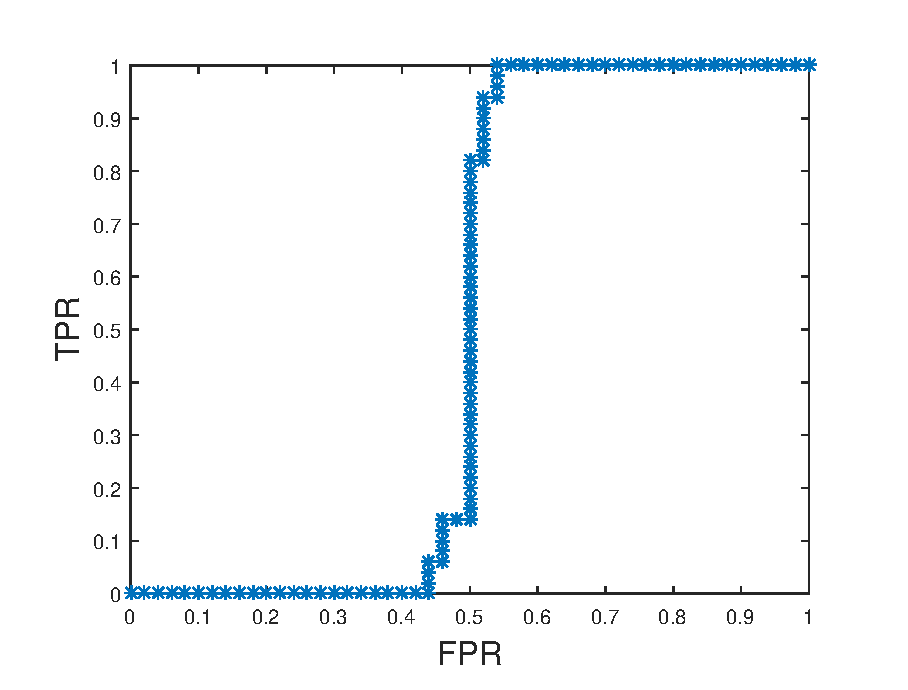
\includegraphics[width=0.6\textwidth]{figuras/prueba.eps}
	\caption{Pie de figura. Poner aquí cita del lugar de donde 
	se ha tomado la imagen en caso de que sea así. }
	\label{fig:prueba}
\end{figure}
\end{verbatim}

% Y ahora pongo la plantilla para que se incluya la figura efectivamente
\begin{figure}[t]
	\centering
	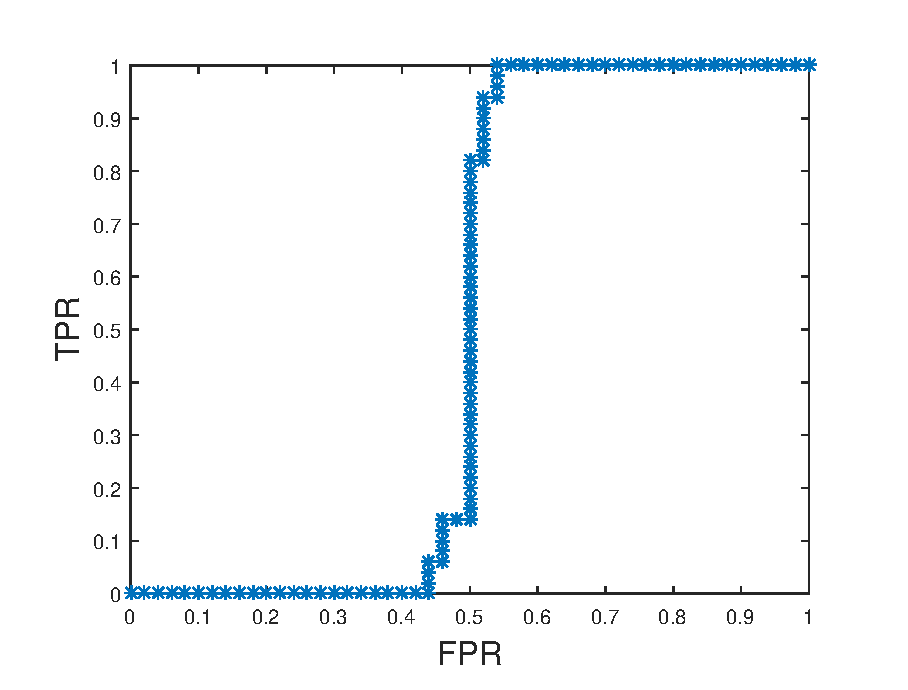
\includegraphics[width=0.6\textwidth]{figuras/prueba.eps}
	\caption{Pie de figura. Poner aquí cita del lugar de donde se ha tomado la imagen en caso de que sea así. }
	\label{fig:prueba}
\end{figure}

Si se pone el modificador [t] (top) latex ubicará la figura en la parte de arriba de la página. Ver otros modificadores como [h] (here) o [b] (bottom). Se pueden usar otras plantillas para, por ejemplo, poner dos figuras una al lado de otra. Consultar en Internet diferentes plantillas en caso de necesidad. 

Cuando en el texto nos refiramos a la figura en cuestión por el número, debemos usar la mayúscula y utilizar referencia a la figura. Esto hará que no nos tengamos que preocupar de la numeración de las figuras. Ej. Como se puede comprobar en la Figura~\ref{fig:prueba}.

Sustituir expresiones del tipo: “En la siguiente figura…” por “En la Figura 2.2…”


\subsection*{Inserción de tablas}

Este sería un ejemplo de una tabla. Se puede modificar el formato y contenido (ver en Internet algún enlace sobre cómo formatear tablas en latex). 

\begin{table}[t]
	\caption{Descripción de la tabla.}
	\label{table:prueba}
	\centering
	\begin{tabular}{l  c} 
		\hline \\[-1.5ex]
		\textbf{Tipo de ataque} & \textbf{Etiqueta} \\ [1ex] 
		\hline\hline \\[-1.5ex]
		DoS11 & dos \\ [0.5ex]
		Exf1MBp & exf1KB \\ [1ex]
		\hline
	\end{tabular}
\end{table}

La forma de referirse a las tablas es similar a las de las figuras (usar mayúsculas y referencia a la etiqueta(label) de la tabla). Ej. Como se puede ver en la Tabla~\ref{table:prueba}, ...


\subsection*{Citas de bibliografía}
Ejemplo de cita de bibliografía. Primero se va a google.scholar y se busca la referencia. Después se da al enlace citar, y se elige el formato bibtex. Se copia ese texto en el fichero bibliografia.bib. Un ejemplo de referenciar una cita es \cite{macia2008evaluation}.


\subsection*{Referencias a secciones}

Para referirnos a secciones, primero debemos tener una etiqueta de tipo \texttt{label} en dicha sección. Posteriormente, pondremos una referencia a dicho label, igual que hacemos para las figuras y las tablas. Ej. Como se ha mencionado en la Sección~\ref{sec:intro:motivacion} (Nótese que la palabra Sección va con mayúscula).

\subsection*{Glosario y acrónimos}

Cuando se utilice un acrónimo se debe definir en el fichero glosario/entradas\_glosario, tal y como está el ejemplo en dicho fichero. Al referirse en el texto se indicará así: \gls{svm} (ver que la primera vez lo pondrá completo). La segunda vez que se referencie a \gls{svm} ya no aparece completo. También se puede nombrar en plural así: \glspl{svm}. 
Otros ejemplos de acrónimo son: \gls{gcd}, \gls{lcm}, \gls{gmf}. 

A la hora de compilar con el glosario, se debe abrir una terminal CMD en el directorio de los fuentes latex del proyecto, y ejecutar el siguiente comando: \texttt{makeglossaries proyecto}. Esto generará los ficheros auxiliares que contienen el glosario. 

\subsection*{Listados de código}

Aquí se puede ver un ejemplo de listado de código: 

%\begin{lstlisting}[frame=none, numbers=none]


\begin{lstlisting}[language=Python,caption=Ejemplo de Python, label=listado:pythonPrueba]
import numpy as np

def incmatrix(genl1,genl2):
	m = len(genl1)
	n = len(genl2)
	M = None #to become the incidence matrix
	VT = np.zeros((n*m,1), int)  #dummy variable

	#compute the bitwise xor matrix
	M1 = bitxormatrix(genl1)
	M2 = np.triu(bitxormatrix(genl2),1) 
	
	for i in range(m-1):
		for j in range(i+1, m):
			[r,c] = np.where(M2 == M1[i,j])
			for k in range(len(r)):
				VT[(i)*n + r[k]] = 1;
				VT[(i)*n + c[k]] = 1;
				VT[(j)*n + r[k]] = 1;
				VT[(j)*n + c[k]] = 1;
	
	if M is None:
		M = np.copy(VT)
	else:
		M = np.concatenate((M, VT), 1)
	
	VT = np.zeros((n*m,1), int)
	
	return M

\end{lstlisting}

Nos podemos referir a él como Listado de código~\ref{listado:pythonPrueba}. 
Si queremos que aparezca como un flotante en la página debemos poner la palabra \texttt{float} así: 
\begin{verbatim}
\begin{lstlisting}[float,language=Python,caption=Ejemplo de Python, 
label=listado:pythonPrueba]
\end{verbatim}


\subsection*{Enlaces URL}
Podemos poner un enlace así \url{http://dtstc.ugr.es/~gmacia} --> %

\chapter*{Guía de estilo para escribir un TFG/TFM} \addcontentsline{toc}{chapter}{Guía de estilo}

Este capítulo no forma parte del TFG/TFM. Su único objetivo es aportar algunas recomendaciones y plantillas para tener claro cómo redactar el TFG/TFM. Una vez se haya comprendido, se puede comentar la siguiente línea en el fichero proyecto.tex añadiéndole al principio el carácter \%: 
\begin{verbatim}
\input{guiaDeEstilo} --> %\input{guiaDeEstilo}
\end{verbatim}

\section*{Recomendaciones generales}
A la hora de escribir el TFG/TFM es importante seguir las siguientes recomendaciones: 

\begin{enumerate}
	\item La memoria debe realizarse con el \textbf{máximo cuidado}, y debe proporcionar de forma consistente -y por sí misma- una idea clara y concisa de lo que se ha realizado. 
	\item No debe tener errores tipográficos ni ortográficos. Este es un aspecto que penaliza muchísimo el trabajo en la evaluación del tribunal. 
	\item Siempre que se utilice alguna figura no elaborada por el autor del proyecto debe indicarse la fuente de la que se ha sacado mediante una cita en la bibliografía. 
	\item La lectura debe ser fluida. Por ello, dada la dificultad que tiene afrontar la escritura de un texto largo casi por primera vez, se recomienda elaborar un índice rellenando los títulos de los diferentes apartados de que constará este documento. En segundo lugar, para cada apartado, se indicarán a modo de resumen las diferentes ideas que se desarrollarán posteriormente (una línea de texto por idea). Después, se desarrollan las ideas (cada idea en un párrafo). Cuando se termina, se realiza una lectura completa y detallada del texto para comprobar que es coherente y no tiene fallos ortográficos, tipográficos ni gramaticales, antes de pasarlo al tutor. 
	\item Una extensión normal está entorno a las 100-120 páginas. Esto no quiere decir que tengamos que escribir por escribir, ni meter contenido adicional sin sentido. Hay que escribir el proyecto de forma coherente, pero sin ser telegráfico, esto es, realizando una descripción detallada del trabajo realizado. 
	\item Evitar afirmaciones del tipo “El sistema diseñado es bastante bueno”. Esa misma frase debería ser escrita tal que responda a las preguntas: ¿Qué parte del sistema? ¿En qué sentido? ¿Cuánto de bueno? ¿Comparado con qué?
	\item Evitar la primera persona (incluso del plural). No obstante para resaltar la autoría de algo o enfatizar una posición personal sí se puede usar.
	\item Numerar estructuradamente los capítulos, secciones y subsecciones. Evitar más de tres niveles de anidamiento. 
	\item Toda afirmación categórica o se demuestra (teórica o experimentalmente)  o se incluye una referencia en la que se haya previamente demostrado.
	\item Toda tecnología, teorema, institución, norma, documento que se mencione debe estar referenciado. No incluir referencias a la wiki.
	\item Los términos en ingles que no tenga sentido traducir se pondrán en cursiva al menos para indicar que es un término no castellano.
	 

\end{enumerate}

\section*{Recomendaciones específicas para determinados contenidos}

\subsection*{Inserción de figuras}
Esta es una plantilla de código para adjuntar una figura. 

% El verbatim es solo para poner en el PDF el código que corresponde a la inserción de la figura
\begin{verbatim}
\begin{figure}[t]
	\centering
		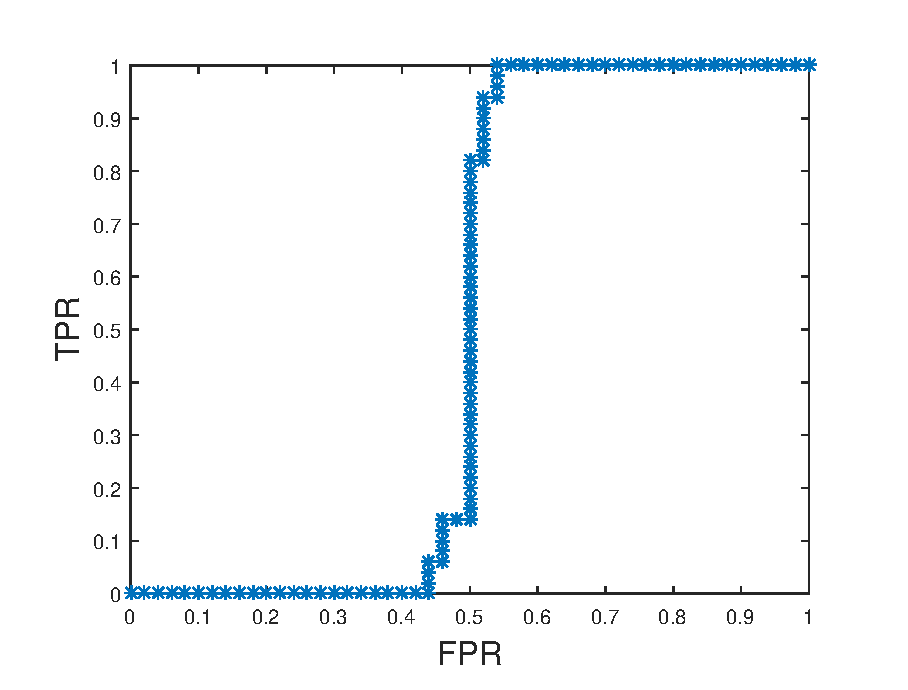
\includegraphics[width=0.6\textwidth]{figuras/prueba.eps}
	\caption{Pie de figura. Poner aquí cita del lugar de donde 
	se ha tomado la imagen en caso de que sea así. }
	\label{fig:prueba}
\end{figure}
\end{verbatim}

% Y ahora pongo la plantilla para que se incluya la figura efectivamente
\begin{figure}[t]
	\centering
	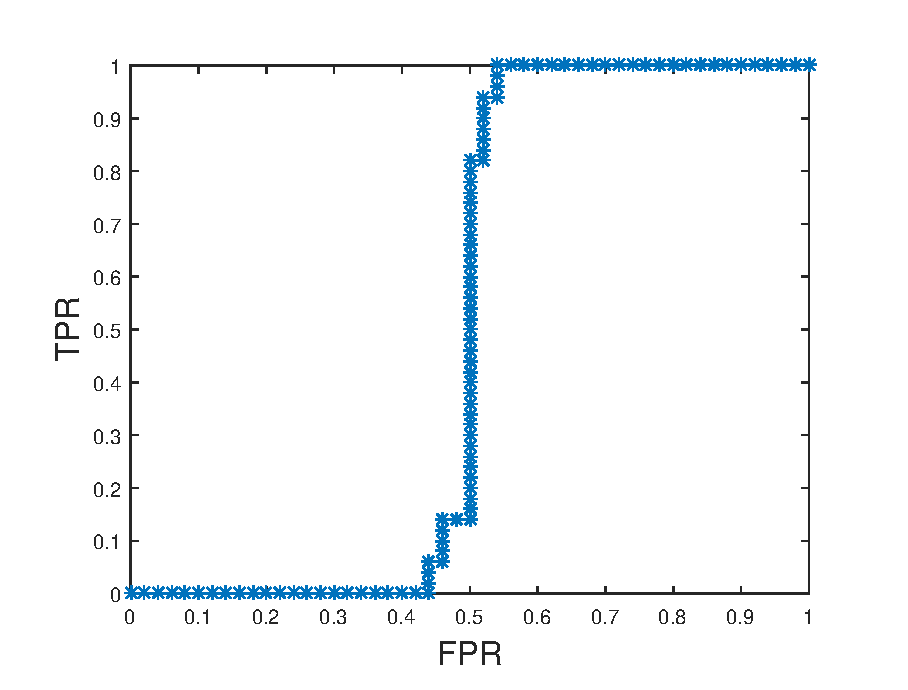
\includegraphics[width=0.6\textwidth]{figuras/prueba.eps}
	\caption{Pie de figura. Poner aquí cita del lugar de donde se ha tomado la imagen en caso de que sea así. }
	\label{fig:prueba}
\end{figure}

Si se pone el modificador [t] (top) latex ubicará la figura en la parte de arriba de la página. Ver otros modificadores como [h] (here) o [b] (bottom). Se pueden usar otras plantillas para, por ejemplo, poner dos figuras una al lado de otra. Consultar en Internet diferentes plantillas en caso de necesidad. 

Cuando en el texto nos refiramos a la figura en cuestión por el número, debemos usar la mayúscula y utilizar referencia a la figura. Esto hará que no nos tengamos que preocupar de la numeración de las figuras. Ej. Como se puede comprobar en la Figura~\ref{fig:prueba}.

Sustituir expresiones del tipo: “En la siguiente figura…” por “En la Figura 2.2…”


\subsection*{Inserción de tablas}

Este sería un ejemplo de una tabla. Se puede modificar el formato y contenido (ver en Internet algún enlace sobre cómo formatear tablas en latex). 

\begin{table}[t]
	\caption{Descripción de la tabla.}
	\label{table:prueba}
	\centering
	\begin{tabular}{l  c} 
		\hline \\[-1.5ex]
		\textbf{Tipo de ataque} & \textbf{Etiqueta} \\ [1ex] 
		\hline\hline \\[-1.5ex]
		DoS11 & dos \\ [0.5ex]
		Exf1MBp & exf1KB \\ [1ex]
		\hline
	\end{tabular}
\end{table}

La forma de referirse a las tablas es similar a las de las figuras (usar mayúsculas y referencia a la etiqueta(label) de la tabla). Ej. Como se puede ver en la Tabla~\ref{table:prueba}, ...


\subsection*{Citas de bibliografía}
Ejemplo de cita de bibliografía. Primero se va a google.scholar y se busca la referencia. Después se da al enlace citar, y se elige el formato bibtex. Se copia ese texto en el fichero bibliografia.bib. Un ejemplo de referenciar una cita es \cite{macia2008evaluation}.


\subsection*{Referencias a secciones}

Para referirnos a secciones, primero debemos tener una etiqueta de tipo \texttt{label} en dicha sección. Posteriormente, pondremos una referencia a dicho label, igual que hacemos para las figuras y las tablas. Ej. Como se ha mencionado en la Sección~\ref{sec:intro:motivacion} (Nótese que la palabra Sección va con mayúscula).

\subsection*{Glosario y acrónimos}

Cuando se utilice un acrónimo se debe definir en el fichero glosario/entradas\_glosario, tal y como está el ejemplo en dicho fichero. Al referirse en el texto se indicará así: \gls{svm} (ver que la primera vez lo pondrá completo). La segunda vez que se referencie a \gls{svm} ya no aparece completo. También se puede nombrar en plural así: \glspl{svm}. 
Otros ejemplos de acrónimo son: \gls{gcd}, \gls{lcm}, \gls{gmf}. 

A la hora de compilar con el glosario, se debe abrir una terminal CMD en el directorio de los fuentes latex del proyecto, y ejecutar el siguiente comando: \texttt{makeglossaries proyecto}. Esto generará los ficheros auxiliares que contienen el glosario. 

\subsection*{Listados de código}

Aquí se puede ver un ejemplo de listado de código: 

%\begin{lstlisting}[frame=none, numbers=none]


\begin{lstlisting}[language=Python,caption=Ejemplo de Python, label=listado:pythonPrueba]
import numpy as np

def incmatrix(genl1,genl2):
	m = len(genl1)
	n = len(genl2)
	M = None #to become the incidence matrix
	VT = np.zeros((n*m,1), int)  #dummy variable

	#compute the bitwise xor matrix
	M1 = bitxormatrix(genl1)
	M2 = np.triu(bitxormatrix(genl2),1) 
	
	for i in range(m-1):
		for j in range(i+1, m):
			[r,c] = np.where(M2 == M1[i,j])
			for k in range(len(r)):
				VT[(i)*n + r[k]] = 1;
				VT[(i)*n + c[k]] = 1;
				VT[(j)*n + r[k]] = 1;
				VT[(j)*n + c[k]] = 1;
	
	if M is None:
		M = np.copy(VT)
	else:
		M = np.concatenate((M, VT), 1)
	
	VT = np.zeros((n*m,1), int)
	
	return M

\end{lstlisting}

Nos podemos referir a él como Listado de código~\ref{listado:pythonPrueba}. 
Si queremos que aparezca como un flotante en la página debemos poner la palabra \texttt{float} así: 
\begin{verbatim}
\begin{lstlisting}[float,language=Python,caption=Ejemplo de Python, 
label=listado:pythonPrueba]
\end{verbatim}


\subsection*{Enlaces URL}
Podemos poner un enlace así \url{http://dtstc.ugr.es/~gmacia}
\end{verbatim}

\section*{Recomendaciones generales}
A la hora de escribir el TFG/TFM es importante seguir las siguientes recomendaciones: 

\begin{enumerate}
	\item La memoria debe realizarse con el \textbf{máximo cuidado}, y debe proporcionar de forma consistente -y por sí misma- una idea clara y concisa de lo que se ha realizado. 
	\item No debe tener errores tipográficos ni ortográficos. Este es un aspecto que penaliza muchísimo el trabajo en la evaluación del tribunal. 
	\item Siempre que se utilice alguna figura no elaborada por el autor del proyecto debe indicarse la fuente de la que se ha sacado mediante una cita en la bibliografía. 
	\item La lectura debe ser fluida. Por ello, dada la dificultad que tiene afrontar la escritura de un texto largo casi por primera vez, se recomienda elaborar un índice rellenando los títulos de los diferentes apartados de que constará este documento. En segundo lugar, para cada apartado, se indicarán a modo de resumen las diferentes ideas que se desarrollarán posteriormente (una línea de texto por idea). Después, se desarrollan las ideas (cada idea en un párrafo). Cuando se termina, se realiza una lectura completa y detallada del texto para comprobar que es coherente y no tiene fallos ortográficos, tipográficos ni gramaticales, antes de pasarlo al tutor. 
	\item Una extensión normal está entorno a las 100-120 páginas. Esto no quiere decir que tengamos que escribir por escribir, ni meter contenido adicional sin sentido. Hay que escribir el proyecto de forma coherente, pero sin ser telegráfico, esto es, realizando una descripción detallada del trabajo realizado. 
	\item Evitar afirmaciones del tipo “El sistema diseñado es bastante bueno”. Esa misma frase debería ser escrita tal que responda a las preguntas: ¿Qué parte del sistema? ¿En qué sentido? ¿Cuánto de bueno? ¿Comparado con qué?
	\item Evitar la primera persona (incluso del plural). No obstante para resaltar la autoría de algo o enfatizar una posición personal sí se puede usar.
	\item Numerar estructuradamente los capítulos, secciones y subsecciones. Evitar más de tres niveles de anidamiento. 
	\item Toda afirmación categórica o se demuestra (teórica o experimentalmente)  o se incluye una referencia en la que se haya previamente demostrado.
	\item Toda tecnología, teorema, institución, norma, documento que se mencione debe estar referenciado. No incluir referencias a la wiki.
	\item Los términos en ingles que no tenga sentido traducir se pondrán en cursiva al menos para indicar que es un término no castellano.
	 

\end{enumerate}

\section*{Recomendaciones específicas para determinados contenidos}

\subsection*{Inserción de figuras}
Esta es una plantilla de código para adjuntar una figura. 

% El verbatim es solo para poner en el PDF el código que corresponde a la inserción de la figura
\begin{verbatim}
\begin{figure}[t]
	\centering
		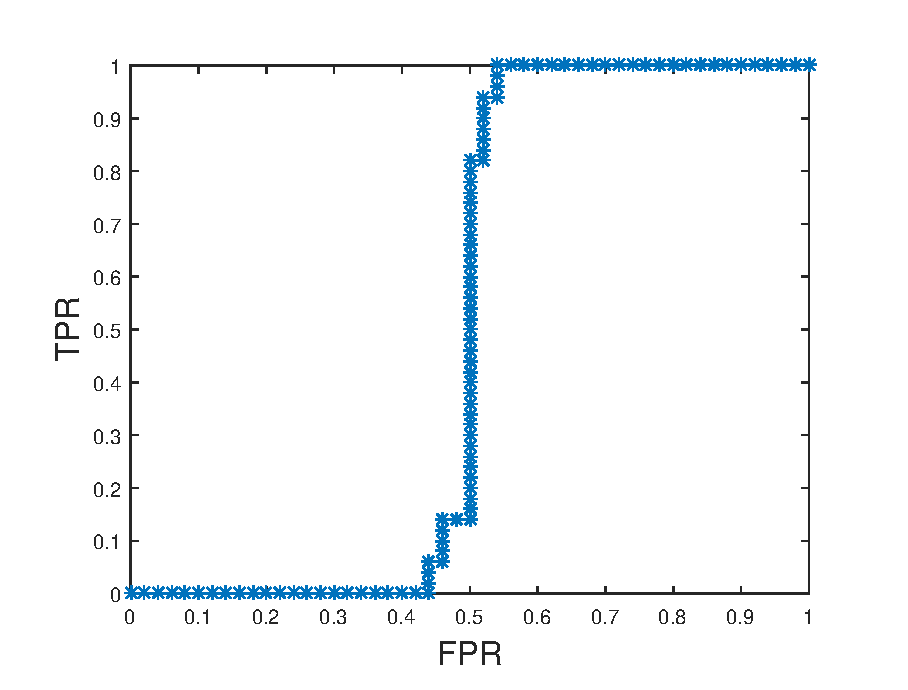
\includegraphics[width=0.6\textwidth]{figuras/prueba.eps}
	\caption{Pie de figura. Poner aquí cita del lugar de donde 
	se ha tomado la imagen en caso de que sea así. }
	\label{fig:prueba}
\end{figure}
\end{verbatim}

% Y ahora pongo la plantilla para que se incluya la figura efectivamente
\begin{figure}[t]
	\centering
	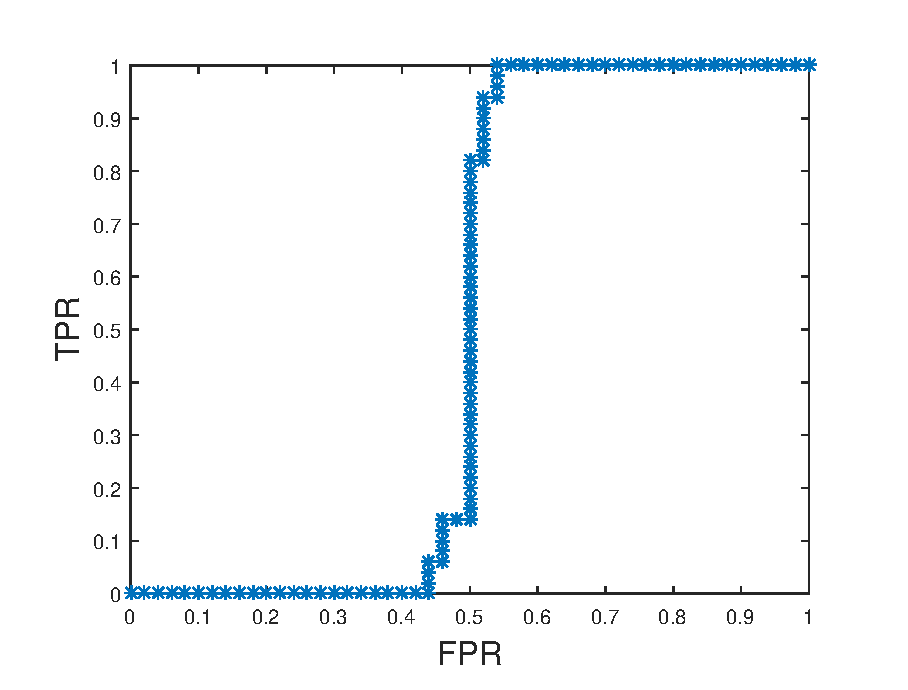
\includegraphics[width=0.6\textwidth]{figuras/prueba.eps}
	\caption{Pie de figura. Poner aquí cita del lugar de donde se ha tomado la imagen en caso de que sea así. }
	\label{fig:prueba}
\end{figure}

Si se pone el modificador [t] (top) latex ubicará la figura en la parte de arriba de la página. Ver otros modificadores como [h] (here) o [b] (bottom). Se pueden usar otras plantillas para, por ejemplo, poner dos figuras una al lado de otra. Consultar en Internet diferentes plantillas en caso de necesidad. 

Cuando en el texto nos refiramos a la figura en cuestión por el número, debemos usar la mayúscula y utilizar referencia a la figura. Esto hará que no nos tengamos que preocupar de la numeración de las figuras. Ej. Como se puede comprobar en la Figura~\ref{fig:prueba}.

Sustituir expresiones del tipo: “En la siguiente figura…” por “En la Figura 2.2…”


\subsection*{Inserción de tablas}

Este sería un ejemplo de una tabla. Se puede modificar el formato y contenido (ver en Internet algún enlace sobre cómo formatear tablas en latex). 

\begin{table}[t]
	\caption{Descripción de la tabla.}
	\label{table:prueba}
	\centering
	\begin{tabular}{l  c} 
		\hline \\[-1.5ex]
		\textbf{Tipo de ataque} & \textbf{Etiqueta} \\ [1ex] 
		\hline\hline \\[-1.5ex]
		DoS11 & dos \\ [0.5ex]
		Exf1MBp & exf1KB \\ [1ex]
		\hline
	\end{tabular}
\end{table}

La forma de referirse a las tablas es similar a las de las figuras (usar mayúsculas y referencia a la etiqueta(label) de la tabla). Ej. Como se puede ver en la Tabla~\ref{table:prueba}, ...


\subsection*{Citas de bibliografía}
Ejemplo de cita de bibliografía. Primero se va a google.scholar y se busca la referencia. Después se da al enlace citar, y se elige el formato bibtex. Se copia ese texto en el fichero bibliografia.bib. Un ejemplo de referenciar una cita es \cite{macia2008evaluation}.


\subsection*{Referencias a secciones}

Para referirnos a secciones, primero debemos tener una etiqueta de tipo \texttt{label} en dicha sección. Posteriormente, pondremos una referencia a dicho label, igual que hacemos para las figuras y las tablas. Ej. Como se ha mencionado en la Sección~\ref{sec:intro:motivacion} (Nótese que la palabra Sección va con mayúscula).

\subsection*{Glosario y acrónimos}

Cuando se utilice un acrónimo se debe definir en el fichero glosario/entradas\_glosario, tal y como está el ejemplo en dicho fichero. Al referirse en el texto se indicará así: \gls{svm} (ver que la primera vez lo pondrá completo). La segunda vez que se referencie a \gls{svm} ya no aparece completo. También se puede nombrar en plural así: \glspl{svm}. 
Otros ejemplos de acrónimo son: \gls{gcd}, \gls{lcm}, \gls{gmf}. 

A la hora de compilar con el glosario, se debe abrir una terminal CMD en el directorio de los fuentes latex del proyecto, y ejecutar el siguiente comando: \texttt{makeglossaries proyecto}. Esto generará los ficheros auxiliares que contienen el glosario. 

\subsection*{Listados de código}

Aquí se puede ver un ejemplo de listado de código: 

%\begin{lstlisting}[frame=none, numbers=none]


\begin{lstlisting}[language=Python,caption=Ejemplo de Python, label=listado:pythonPrueba]
import numpy as np

def incmatrix(genl1,genl2):
	m = len(genl1)
	n = len(genl2)
	M = None #to become the incidence matrix
	VT = np.zeros((n*m,1), int)  #dummy variable

	#compute the bitwise xor matrix
	M1 = bitxormatrix(genl1)
	M2 = np.triu(bitxormatrix(genl2),1) 
	
	for i in range(m-1):
		for j in range(i+1, m):
			[r,c] = np.where(M2 == M1[i,j])
			for k in range(len(r)):
				VT[(i)*n + r[k]] = 1;
				VT[(i)*n + c[k]] = 1;
				VT[(j)*n + r[k]] = 1;
				VT[(j)*n + c[k]] = 1;
	
	if M is None:
		M = np.copy(VT)
	else:
		M = np.concatenate((M, VT), 1)
	
	VT = np.zeros((n*m,1), int)
	
	return M

\end{lstlisting}

Nos podemos referir a él como Listado de código~\ref{listado:pythonPrueba}. 
Si queremos que aparezca como un flotante en la página debemos poner la palabra \texttt{float} así: 
\begin{verbatim}
\begin{lstlisting}[float,language=Python,caption=Ejemplo de Python, 
label=listado:pythonPrueba]
\end{verbatim}


\subsection*{Enlaces URL}
Podemos poner un enlace así \url{http://dtstc.ugr.es/~gmacia} --> %

\chapter*{Guía de estilo para escribir un TFG/TFM} \addcontentsline{toc}{chapter}{Guía de estilo}

Este capítulo no forma parte del TFG/TFM. Su único objetivo es aportar algunas recomendaciones y plantillas para tener claro cómo redactar el TFG/TFM. Una vez se haya comprendido, se puede comentar la siguiente línea en el fichero proyecto.tex añadiéndole al principio el carácter \%: 
\begin{verbatim}


\chapter*{Guía de estilo para escribir un TFG/TFM} \addcontentsline{toc}{chapter}{Guía de estilo}

Este capítulo no forma parte del TFG/TFM. Su único objetivo es aportar algunas recomendaciones y plantillas para tener claro cómo redactar el TFG/TFM. Una vez se haya comprendido, se puede comentar la siguiente línea en el fichero proyecto.tex añadiéndole al principio el carácter \%: 
\begin{verbatim}
\input{guiaDeEstilo} --> %\input{guiaDeEstilo}
\end{verbatim}

\section*{Recomendaciones generales}
A la hora de escribir el TFG/TFM es importante seguir las siguientes recomendaciones: 

\begin{enumerate}
	\item La memoria debe realizarse con el \textbf{máximo cuidado}, y debe proporcionar de forma consistente -y por sí misma- una idea clara y concisa de lo que se ha realizado. 
	\item No debe tener errores tipográficos ni ortográficos. Este es un aspecto que penaliza muchísimo el trabajo en la evaluación del tribunal. 
	\item Siempre que se utilice alguna figura no elaborada por el autor del proyecto debe indicarse la fuente de la que se ha sacado mediante una cita en la bibliografía. 
	\item La lectura debe ser fluida. Por ello, dada la dificultad que tiene afrontar la escritura de un texto largo casi por primera vez, se recomienda elaborar un índice rellenando los títulos de los diferentes apartados de que constará este documento. En segundo lugar, para cada apartado, se indicarán a modo de resumen las diferentes ideas que se desarrollarán posteriormente (una línea de texto por idea). Después, se desarrollan las ideas (cada idea en un párrafo). Cuando se termina, se realiza una lectura completa y detallada del texto para comprobar que es coherente y no tiene fallos ortográficos, tipográficos ni gramaticales, antes de pasarlo al tutor. 
	\item Una extensión normal está entorno a las 100-120 páginas. Esto no quiere decir que tengamos que escribir por escribir, ni meter contenido adicional sin sentido. Hay que escribir el proyecto de forma coherente, pero sin ser telegráfico, esto es, realizando una descripción detallada del trabajo realizado. 
	\item Evitar afirmaciones del tipo “El sistema diseñado es bastante bueno”. Esa misma frase debería ser escrita tal que responda a las preguntas: ¿Qué parte del sistema? ¿En qué sentido? ¿Cuánto de bueno? ¿Comparado con qué?
	\item Evitar la primera persona (incluso del plural). No obstante para resaltar la autoría de algo o enfatizar una posición personal sí se puede usar.
	\item Numerar estructuradamente los capítulos, secciones y subsecciones. Evitar más de tres niveles de anidamiento. 
	\item Toda afirmación categórica o se demuestra (teórica o experimentalmente)  o se incluye una referencia en la que se haya previamente demostrado.
	\item Toda tecnología, teorema, institución, norma, documento que se mencione debe estar referenciado. No incluir referencias a la wiki.
	\item Los términos en ingles que no tenga sentido traducir se pondrán en cursiva al menos para indicar que es un término no castellano.
	 

\end{enumerate}

\section*{Recomendaciones específicas para determinados contenidos}

\subsection*{Inserción de figuras}
Esta es una plantilla de código para adjuntar una figura. 

% El verbatim es solo para poner en el PDF el código que corresponde a la inserción de la figura
\begin{verbatim}
\begin{figure}[t]
	\centering
		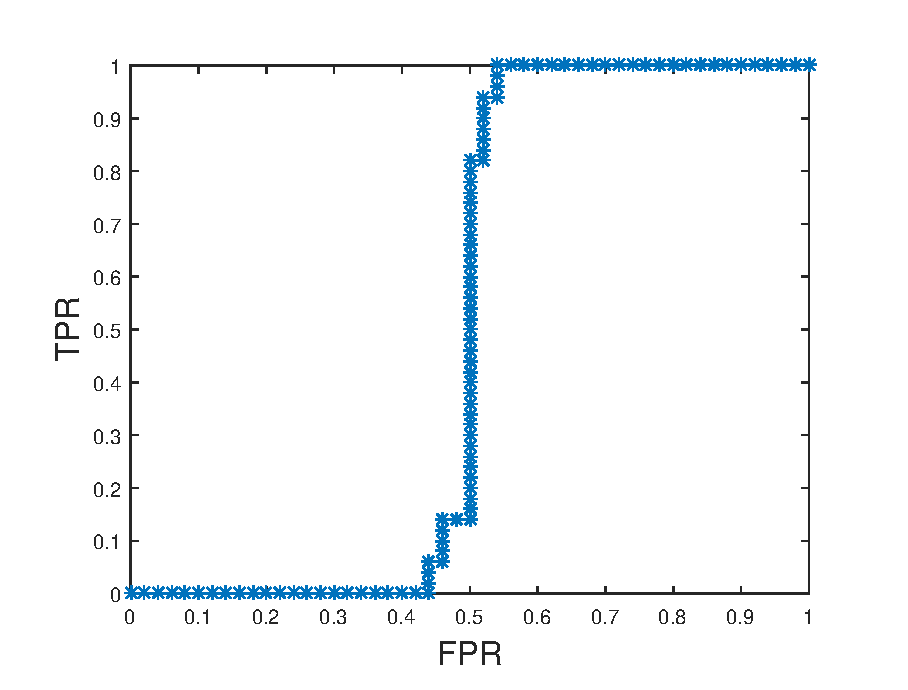
\includegraphics[width=0.6\textwidth]{figuras/prueba.eps}
	\caption{Pie de figura. Poner aquí cita del lugar de donde 
	se ha tomado la imagen en caso de que sea así. }
	\label{fig:prueba}
\end{figure}
\end{verbatim}

% Y ahora pongo la plantilla para que se incluya la figura efectivamente
\begin{figure}[t]
	\centering
	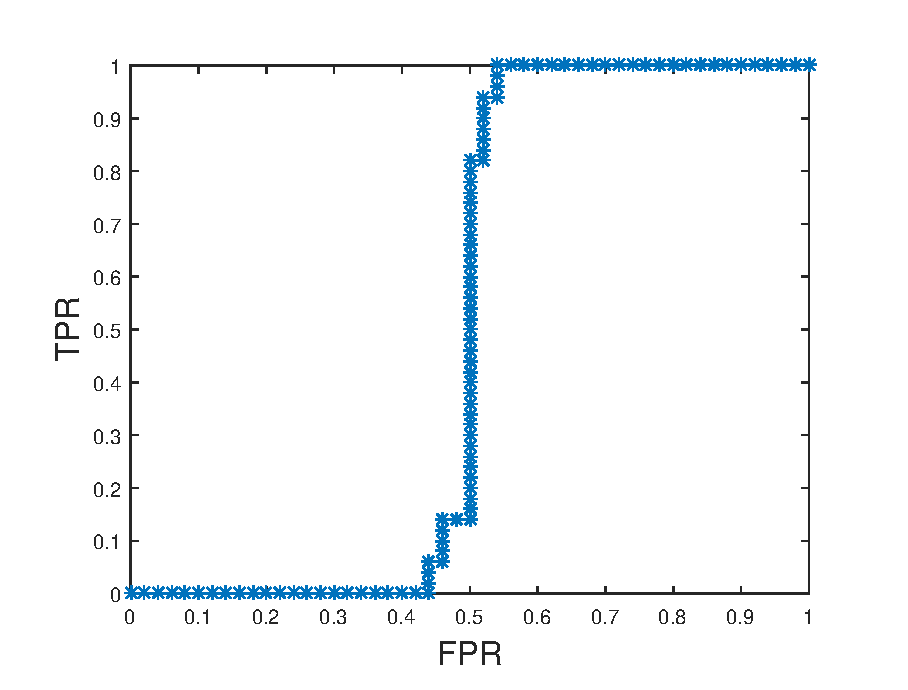
\includegraphics[width=0.6\textwidth]{figuras/prueba.eps}
	\caption{Pie de figura. Poner aquí cita del lugar de donde se ha tomado la imagen en caso de que sea así. }
	\label{fig:prueba}
\end{figure}

Si se pone el modificador [t] (top) latex ubicará la figura en la parte de arriba de la página. Ver otros modificadores como [h] (here) o [b] (bottom). Se pueden usar otras plantillas para, por ejemplo, poner dos figuras una al lado de otra. Consultar en Internet diferentes plantillas en caso de necesidad. 

Cuando en el texto nos refiramos a la figura en cuestión por el número, debemos usar la mayúscula y utilizar referencia a la figura. Esto hará que no nos tengamos que preocupar de la numeración de las figuras. Ej. Como se puede comprobar en la Figura~\ref{fig:prueba}.

Sustituir expresiones del tipo: “En la siguiente figura…” por “En la Figura 2.2…”


\subsection*{Inserción de tablas}

Este sería un ejemplo de una tabla. Se puede modificar el formato y contenido (ver en Internet algún enlace sobre cómo formatear tablas en latex). 

\begin{table}[t]
	\caption{Descripción de la tabla.}
	\label{table:prueba}
	\centering
	\begin{tabular}{l  c} 
		\hline \\[-1.5ex]
		\textbf{Tipo de ataque} & \textbf{Etiqueta} \\ [1ex] 
		\hline\hline \\[-1.5ex]
		DoS11 & dos \\ [0.5ex]
		Exf1MBp & exf1KB \\ [1ex]
		\hline
	\end{tabular}
\end{table}

La forma de referirse a las tablas es similar a las de las figuras (usar mayúsculas y referencia a la etiqueta(label) de la tabla). Ej. Como se puede ver en la Tabla~\ref{table:prueba}, ...


\subsection*{Citas de bibliografía}
Ejemplo de cita de bibliografía. Primero se va a google.scholar y se busca la referencia. Después se da al enlace citar, y se elige el formato bibtex. Se copia ese texto en el fichero bibliografia.bib. Un ejemplo de referenciar una cita es \cite{macia2008evaluation}.


\subsection*{Referencias a secciones}

Para referirnos a secciones, primero debemos tener una etiqueta de tipo \texttt{label} en dicha sección. Posteriormente, pondremos una referencia a dicho label, igual que hacemos para las figuras y las tablas. Ej. Como se ha mencionado en la Sección~\ref{sec:intro:motivacion} (Nótese que la palabra Sección va con mayúscula).

\subsection*{Glosario y acrónimos}

Cuando se utilice un acrónimo se debe definir en el fichero glosario/entradas\_glosario, tal y como está el ejemplo en dicho fichero. Al referirse en el texto se indicará así: \gls{svm} (ver que la primera vez lo pondrá completo). La segunda vez que se referencie a \gls{svm} ya no aparece completo. También se puede nombrar en plural así: \glspl{svm}. 
Otros ejemplos de acrónimo son: \gls{gcd}, \gls{lcm}, \gls{gmf}. 

A la hora de compilar con el glosario, se debe abrir una terminal CMD en el directorio de los fuentes latex del proyecto, y ejecutar el siguiente comando: \texttt{makeglossaries proyecto}. Esto generará los ficheros auxiliares que contienen el glosario. 

\subsection*{Listados de código}

Aquí se puede ver un ejemplo de listado de código: 

%\begin{lstlisting}[frame=none, numbers=none]


\begin{lstlisting}[language=Python,caption=Ejemplo de Python, label=listado:pythonPrueba]
import numpy as np

def incmatrix(genl1,genl2):
	m = len(genl1)
	n = len(genl2)
	M = None #to become the incidence matrix
	VT = np.zeros((n*m,1), int)  #dummy variable

	#compute the bitwise xor matrix
	M1 = bitxormatrix(genl1)
	M2 = np.triu(bitxormatrix(genl2),1) 
	
	for i in range(m-1):
		for j in range(i+1, m):
			[r,c] = np.where(M2 == M1[i,j])
			for k in range(len(r)):
				VT[(i)*n + r[k]] = 1;
				VT[(i)*n + c[k]] = 1;
				VT[(j)*n + r[k]] = 1;
				VT[(j)*n + c[k]] = 1;
	
	if M is None:
		M = np.copy(VT)
	else:
		M = np.concatenate((M, VT), 1)
	
	VT = np.zeros((n*m,1), int)
	
	return M

\end{lstlisting}

Nos podemos referir a él como Listado de código~\ref{listado:pythonPrueba}. 
Si queremos que aparezca como un flotante en la página debemos poner la palabra \texttt{float} así: 
\begin{verbatim}
\begin{lstlisting}[float,language=Python,caption=Ejemplo de Python, 
label=listado:pythonPrueba]
\end{verbatim}


\subsection*{Enlaces URL}
Podemos poner un enlace así \url{http://dtstc.ugr.es/~gmacia} --> %

\chapter*{Guía de estilo para escribir un TFG/TFM} \addcontentsline{toc}{chapter}{Guía de estilo}

Este capítulo no forma parte del TFG/TFM. Su único objetivo es aportar algunas recomendaciones y plantillas para tener claro cómo redactar el TFG/TFM. Una vez se haya comprendido, se puede comentar la siguiente línea en el fichero proyecto.tex añadiéndole al principio el carácter \%: 
\begin{verbatim}
\input{guiaDeEstilo} --> %\input{guiaDeEstilo}
\end{verbatim}

\section*{Recomendaciones generales}
A la hora de escribir el TFG/TFM es importante seguir las siguientes recomendaciones: 

\begin{enumerate}
	\item La memoria debe realizarse con el \textbf{máximo cuidado}, y debe proporcionar de forma consistente -y por sí misma- una idea clara y concisa de lo que se ha realizado. 
	\item No debe tener errores tipográficos ni ortográficos. Este es un aspecto que penaliza muchísimo el trabajo en la evaluación del tribunal. 
	\item Siempre que se utilice alguna figura no elaborada por el autor del proyecto debe indicarse la fuente de la que se ha sacado mediante una cita en la bibliografía. 
	\item La lectura debe ser fluida. Por ello, dada la dificultad que tiene afrontar la escritura de un texto largo casi por primera vez, se recomienda elaborar un índice rellenando los títulos de los diferentes apartados de que constará este documento. En segundo lugar, para cada apartado, se indicarán a modo de resumen las diferentes ideas que se desarrollarán posteriormente (una línea de texto por idea). Después, se desarrollan las ideas (cada idea en un párrafo). Cuando se termina, se realiza una lectura completa y detallada del texto para comprobar que es coherente y no tiene fallos ortográficos, tipográficos ni gramaticales, antes de pasarlo al tutor. 
	\item Una extensión normal está entorno a las 100-120 páginas. Esto no quiere decir que tengamos que escribir por escribir, ni meter contenido adicional sin sentido. Hay que escribir el proyecto de forma coherente, pero sin ser telegráfico, esto es, realizando una descripción detallada del trabajo realizado. 
	\item Evitar afirmaciones del tipo “El sistema diseñado es bastante bueno”. Esa misma frase debería ser escrita tal que responda a las preguntas: ¿Qué parte del sistema? ¿En qué sentido? ¿Cuánto de bueno? ¿Comparado con qué?
	\item Evitar la primera persona (incluso del plural). No obstante para resaltar la autoría de algo o enfatizar una posición personal sí se puede usar.
	\item Numerar estructuradamente los capítulos, secciones y subsecciones. Evitar más de tres niveles de anidamiento. 
	\item Toda afirmación categórica o se demuestra (teórica o experimentalmente)  o se incluye una referencia en la que se haya previamente demostrado.
	\item Toda tecnología, teorema, institución, norma, documento que se mencione debe estar referenciado. No incluir referencias a la wiki.
	\item Los términos en ingles que no tenga sentido traducir se pondrán en cursiva al menos para indicar que es un término no castellano.
	 

\end{enumerate}

\section*{Recomendaciones específicas para determinados contenidos}

\subsection*{Inserción de figuras}
Esta es una plantilla de código para adjuntar una figura. 

% El verbatim es solo para poner en el PDF el código que corresponde a la inserción de la figura
\begin{verbatim}
\begin{figure}[t]
	\centering
		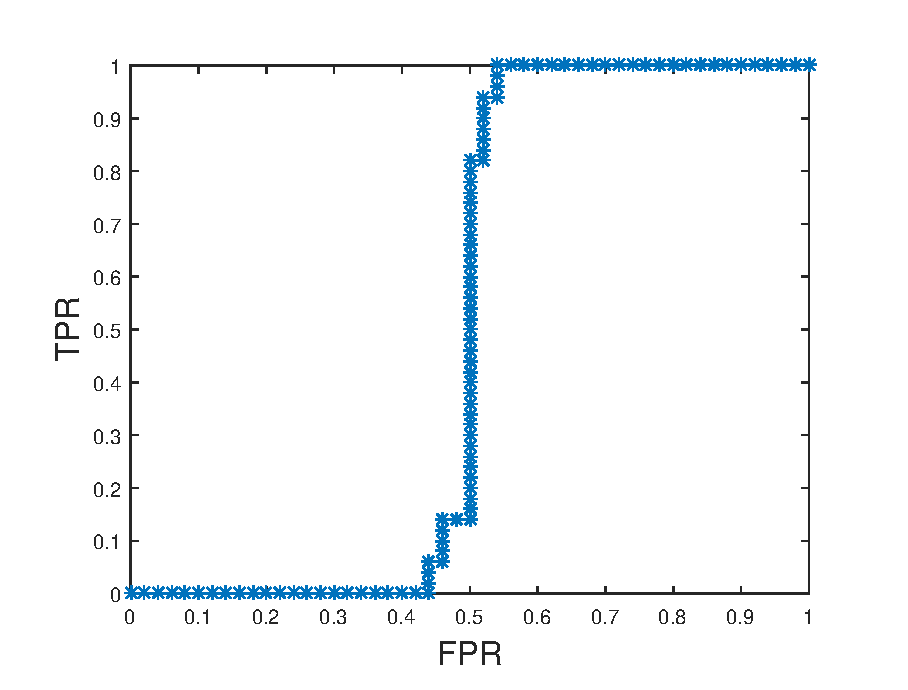
\includegraphics[width=0.6\textwidth]{figuras/prueba.eps}
	\caption{Pie de figura. Poner aquí cita del lugar de donde 
	se ha tomado la imagen en caso de que sea así. }
	\label{fig:prueba}
\end{figure}
\end{verbatim}

% Y ahora pongo la plantilla para que se incluya la figura efectivamente
\begin{figure}[t]
	\centering
	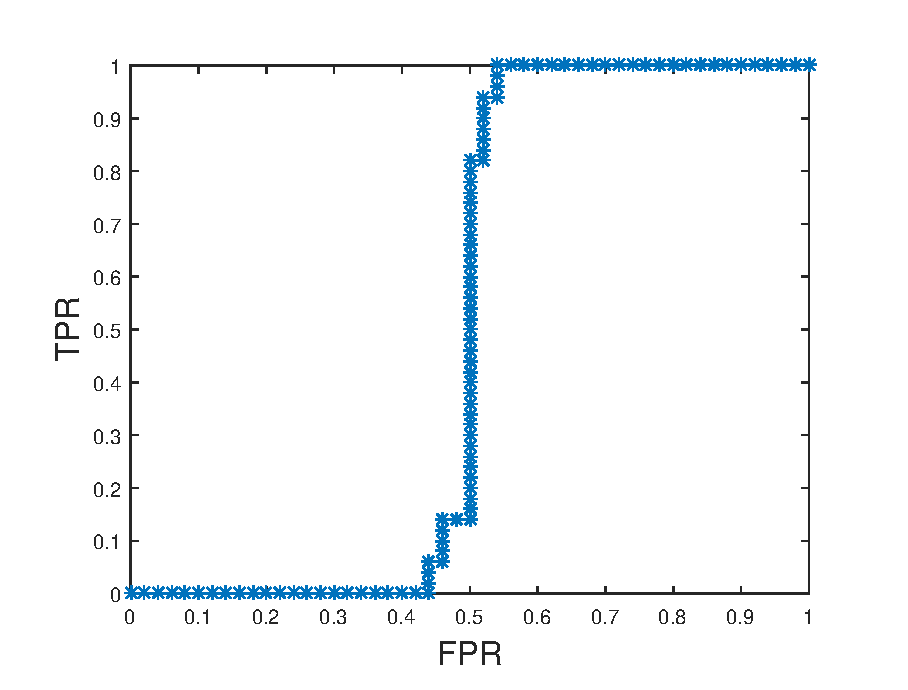
\includegraphics[width=0.6\textwidth]{figuras/prueba.eps}
	\caption{Pie de figura. Poner aquí cita del lugar de donde se ha tomado la imagen en caso de que sea así. }
	\label{fig:prueba}
\end{figure}

Si se pone el modificador [t] (top) latex ubicará la figura en la parte de arriba de la página. Ver otros modificadores como [h] (here) o [b] (bottom). Se pueden usar otras plantillas para, por ejemplo, poner dos figuras una al lado de otra. Consultar en Internet diferentes plantillas en caso de necesidad. 

Cuando en el texto nos refiramos a la figura en cuestión por el número, debemos usar la mayúscula y utilizar referencia a la figura. Esto hará que no nos tengamos que preocupar de la numeración de las figuras. Ej. Como se puede comprobar en la Figura~\ref{fig:prueba}.

Sustituir expresiones del tipo: “En la siguiente figura…” por “En la Figura 2.2…”


\subsection*{Inserción de tablas}

Este sería un ejemplo de una tabla. Se puede modificar el formato y contenido (ver en Internet algún enlace sobre cómo formatear tablas en latex). 

\begin{table}[t]
	\caption{Descripción de la tabla.}
	\label{table:prueba}
	\centering
	\begin{tabular}{l  c} 
		\hline \\[-1.5ex]
		\textbf{Tipo de ataque} & \textbf{Etiqueta} \\ [1ex] 
		\hline\hline \\[-1.5ex]
		DoS11 & dos \\ [0.5ex]
		Exf1MBp & exf1KB \\ [1ex]
		\hline
	\end{tabular}
\end{table}

La forma de referirse a las tablas es similar a las de las figuras (usar mayúsculas y referencia a la etiqueta(label) de la tabla). Ej. Como se puede ver en la Tabla~\ref{table:prueba}, ...


\subsection*{Citas de bibliografía}
Ejemplo de cita de bibliografía. Primero se va a google.scholar y se busca la referencia. Después se da al enlace citar, y se elige el formato bibtex. Se copia ese texto en el fichero bibliografia.bib. Un ejemplo de referenciar una cita es \cite{macia2008evaluation}.


\subsection*{Referencias a secciones}

Para referirnos a secciones, primero debemos tener una etiqueta de tipo \texttt{label} en dicha sección. Posteriormente, pondremos una referencia a dicho label, igual que hacemos para las figuras y las tablas. Ej. Como se ha mencionado en la Sección~\ref{sec:intro:motivacion} (Nótese que la palabra Sección va con mayúscula).

\subsection*{Glosario y acrónimos}

Cuando se utilice un acrónimo se debe definir en el fichero glosario/entradas\_glosario, tal y como está el ejemplo en dicho fichero. Al referirse en el texto se indicará así: \gls{svm} (ver que la primera vez lo pondrá completo). La segunda vez que se referencie a \gls{svm} ya no aparece completo. También se puede nombrar en plural así: \glspl{svm}. 
Otros ejemplos de acrónimo son: \gls{gcd}, \gls{lcm}, \gls{gmf}. 

A la hora de compilar con el glosario, se debe abrir una terminal CMD en el directorio de los fuentes latex del proyecto, y ejecutar el siguiente comando: \texttt{makeglossaries proyecto}. Esto generará los ficheros auxiliares que contienen el glosario. 

\subsection*{Listados de código}

Aquí se puede ver un ejemplo de listado de código: 

%\begin{lstlisting}[frame=none, numbers=none]


\begin{lstlisting}[language=Python,caption=Ejemplo de Python, label=listado:pythonPrueba]
import numpy as np

def incmatrix(genl1,genl2):
	m = len(genl1)
	n = len(genl2)
	M = None #to become the incidence matrix
	VT = np.zeros((n*m,1), int)  #dummy variable

	#compute the bitwise xor matrix
	M1 = bitxormatrix(genl1)
	M2 = np.triu(bitxormatrix(genl2),1) 
	
	for i in range(m-1):
		for j in range(i+1, m):
			[r,c] = np.where(M2 == M1[i,j])
			for k in range(len(r)):
				VT[(i)*n + r[k]] = 1;
				VT[(i)*n + c[k]] = 1;
				VT[(j)*n + r[k]] = 1;
				VT[(j)*n + c[k]] = 1;
	
	if M is None:
		M = np.copy(VT)
	else:
		M = np.concatenate((M, VT), 1)
	
	VT = np.zeros((n*m,1), int)
	
	return M

\end{lstlisting}

Nos podemos referir a él como Listado de código~\ref{listado:pythonPrueba}. 
Si queremos que aparezca como un flotante en la página debemos poner la palabra \texttt{float} así: 
\begin{verbatim}
\begin{lstlisting}[float,language=Python,caption=Ejemplo de Python, 
label=listado:pythonPrueba]
\end{verbatim}


\subsection*{Enlaces URL}
Podemos poner un enlace así \url{http://dtstc.ugr.es/~gmacia}
\end{verbatim}

\section*{Recomendaciones generales}
A la hora de escribir el TFG/TFM es importante seguir las siguientes recomendaciones: 

\begin{enumerate}
	\item La memoria debe realizarse con el \textbf{máximo cuidado}, y debe proporcionar de forma consistente -y por sí misma- una idea clara y concisa de lo que se ha realizado. 
	\item No debe tener errores tipográficos ni ortográficos. Este es un aspecto que penaliza muchísimo el trabajo en la evaluación del tribunal. 
	\item Siempre que se utilice alguna figura no elaborada por el autor del proyecto debe indicarse la fuente de la que se ha sacado mediante una cita en la bibliografía. 
	\item La lectura debe ser fluida. Por ello, dada la dificultad que tiene afrontar la escritura de un texto largo casi por primera vez, se recomienda elaborar un índice rellenando los títulos de los diferentes apartados de que constará este documento. En segundo lugar, para cada apartado, se indicarán a modo de resumen las diferentes ideas que se desarrollarán posteriormente (una línea de texto por idea). Después, se desarrollan las ideas (cada idea en un párrafo). Cuando se termina, se realiza una lectura completa y detallada del texto para comprobar que es coherente y no tiene fallos ortográficos, tipográficos ni gramaticales, antes de pasarlo al tutor. 
	\item Una extensión normal está entorno a las 100-120 páginas. Esto no quiere decir que tengamos que escribir por escribir, ni meter contenido adicional sin sentido. Hay que escribir el proyecto de forma coherente, pero sin ser telegráfico, esto es, realizando una descripción detallada del trabajo realizado. 
	\item Evitar afirmaciones del tipo “El sistema diseñado es bastante bueno”. Esa misma frase debería ser escrita tal que responda a las preguntas: ¿Qué parte del sistema? ¿En qué sentido? ¿Cuánto de bueno? ¿Comparado con qué?
	\item Evitar la primera persona (incluso del plural). No obstante para resaltar la autoría de algo o enfatizar una posición personal sí se puede usar.
	\item Numerar estructuradamente los capítulos, secciones y subsecciones. Evitar más de tres niveles de anidamiento. 
	\item Toda afirmación categórica o se demuestra (teórica o experimentalmente)  o se incluye una referencia en la que se haya previamente demostrado.
	\item Toda tecnología, teorema, institución, norma, documento que se mencione debe estar referenciado. No incluir referencias a la wiki.
	\item Los términos en ingles que no tenga sentido traducir se pondrán en cursiva al menos para indicar que es un término no castellano.
	 

\end{enumerate}

\section*{Recomendaciones específicas para determinados contenidos}

\subsection*{Inserción de figuras}
Esta es una plantilla de código para adjuntar una figura. 

% El verbatim es solo para poner en el PDF el código que corresponde a la inserción de la figura
\begin{verbatim}
\begin{figure}[t]
	\centering
		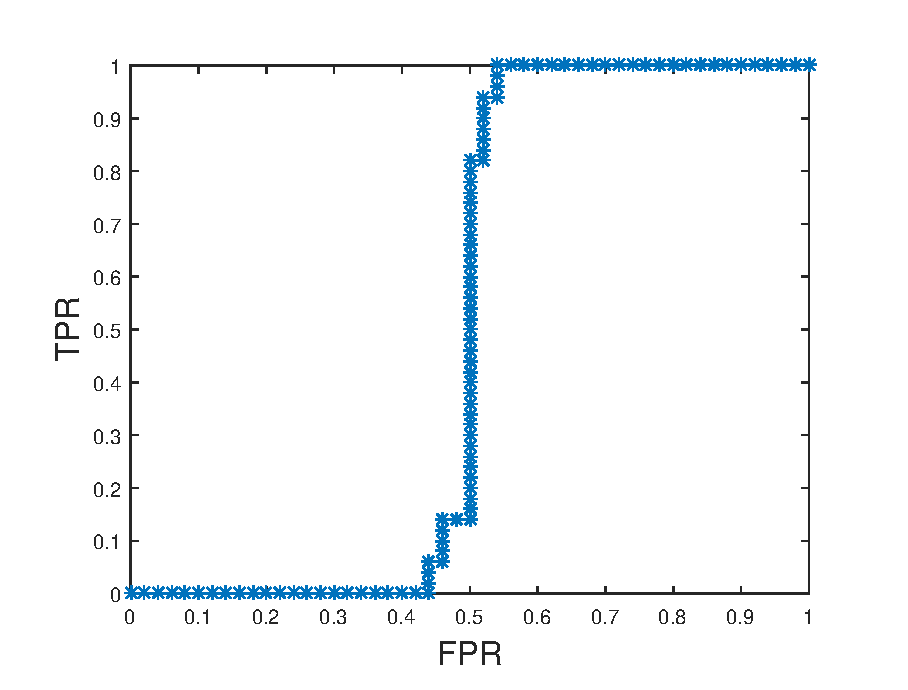
\includegraphics[width=0.6\textwidth]{figuras/prueba.eps}
	\caption{Pie de figura. Poner aquí cita del lugar de donde 
	se ha tomado la imagen en caso de que sea así. }
	\label{fig:prueba}
\end{figure}
\end{verbatim}

% Y ahora pongo la plantilla para que se incluya la figura efectivamente
\begin{figure}[t]
	\centering
	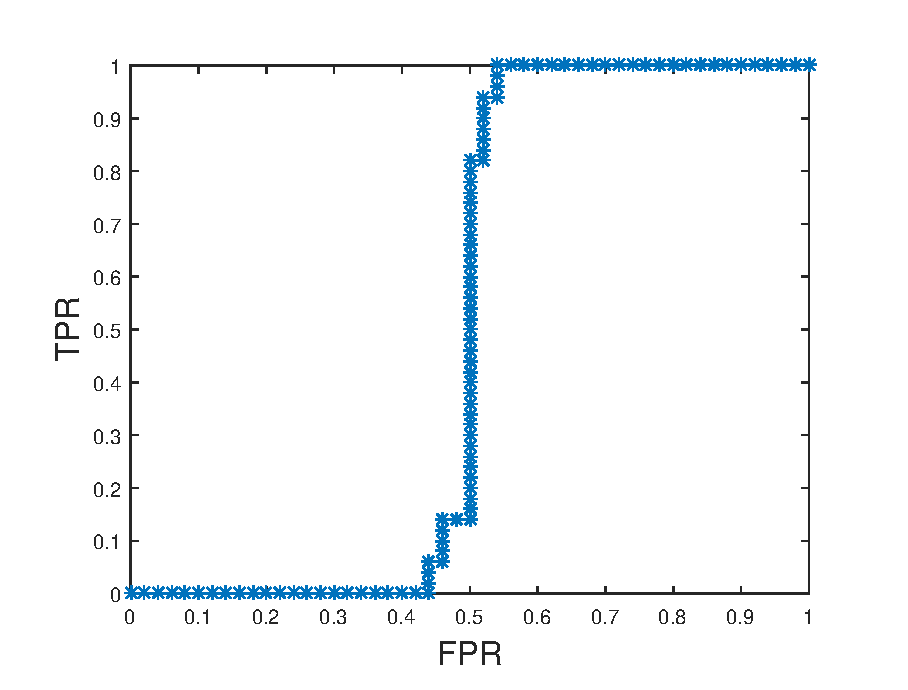
\includegraphics[width=0.6\textwidth]{figuras/prueba.eps}
	\caption{Pie de figura. Poner aquí cita del lugar de donde se ha tomado la imagen en caso de que sea así. }
	\label{fig:prueba}
\end{figure}

Si se pone el modificador [t] (top) latex ubicará la figura en la parte de arriba de la página. Ver otros modificadores como [h] (here) o [b] (bottom). Se pueden usar otras plantillas para, por ejemplo, poner dos figuras una al lado de otra. Consultar en Internet diferentes plantillas en caso de necesidad. 

Cuando en el texto nos refiramos a la figura en cuestión por el número, debemos usar la mayúscula y utilizar referencia a la figura. Esto hará que no nos tengamos que preocupar de la numeración de las figuras. Ej. Como se puede comprobar en la Figura~\ref{fig:prueba}.

Sustituir expresiones del tipo: “En la siguiente figura…” por “En la Figura 2.2…”


\subsection*{Inserción de tablas}

Este sería un ejemplo de una tabla. Se puede modificar el formato y contenido (ver en Internet algún enlace sobre cómo formatear tablas en latex). 

\begin{table}[t]
	\caption{Descripción de la tabla.}
	\label{table:prueba}
	\centering
	\begin{tabular}{l  c} 
		\hline \\[-1.5ex]
		\textbf{Tipo de ataque} & \textbf{Etiqueta} \\ [1ex] 
		\hline\hline \\[-1.5ex]
		DoS11 & dos \\ [0.5ex]
		Exf1MBp & exf1KB \\ [1ex]
		\hline
	\end{tabular}
\end{table}

La forma de referirse a las tablas es similar a las de las figuras (usar mayúsculas y referencia a la etiqueta(label) de la tabla). Ej. Como se puede ver en la Tabla~\ref{table:prueba}, ...


\subsection*{Citas de bibliografía}
Ejemplo de cita de bibliografía. Primero se va a google.scholar y se busca la referencia. Después se da al enlace citar, y se elige el formato bibtex. Se copia ese texto en el fichero bibliografia.bib. Un ejemplo de referenciar una cita es \cite{macia2008evaluation}.


\subsection*{Referencias a secciones}

Para referirnos a secciones, primero debemos tener una etiqueta de tipo \texttt{label} en dicha sección. Posteriormente, pondremos una referencia a dicho label, igual que hacemos para las figuras y las tablas. Ej. Como se ha mencionado en la Sección~\ref{sec:intro:motivacion} (Nótese que la palabra Sección va con mayúscula).

\subsection*{Glosario y acrónimos}

Cuando se utilice un acrónimo se debe definir en el fichero glosario/entradas\_glosario, tal y como está el ejemplo en dicho fichero. Al referirse en el texto se indicará así: \gls{svm} (ver que la primera vez lo pondrá completo). La segunda vez que se referencie a \gls{svm} ya no aparece completo. También se puede nombrar en plural así: \glspl{svm}. 
Otros ejemplos de acrónimo son: \gls{gcd}, \gls{lcm}, \gls{gmf}. 

A la hora de compilar con el glosario, se debe abrir una terminal CMD en el directorio de los fuentes latex del proyecto, y ejecutar el siguiente comando: \texttt{makeglossaries proyecto}. Esto generará los ficheros auxiliares que contienen el glosario. 

\subsection*{Listados de código}

Aquí se puede ver un ejemplo de listado de código: 

%\begin{lstlisting}[frame=none, numbers=none]


\begin{lstlisting}[language=Python,caption=Ejemplo de Python, label=listado:pythonPrueba]
import numpy as np

def incmatrix(genl1,genl2):
	m = len(genl1)
	n = len(genl2)
	M = None #to become the incidence matrix
	VT = np.zeros((n*m,1), int)  #dummy variable

	#compute the bitwise xor matrix
	M1 = bitxormatrix(genl1)
	M2 = np.triu(bitxormatrix(genl2),1) 
	
	for i in range(m-1):
		for j in range(i+1, m):
			[r,c] = np.where(M2 == M1[i,j])
			for k in range(len(r)):
				VT[(i)*n + r[k]] = 1;
				VT[(i)*n + c[k]] = 1;
				VT[(j)*n + r[k]] = 1;
				VT[(j)*n + c[k]] = 1;
	
	if M is None:
		M = np.copy(VT)
	else:
		M = np.concatenate((M, VT), 1)
	
	VT = np.zeros((n*m,1), int)
	
	return M

\end{lstlisting}

Nos podemos referir a él como Listado de código~\ref{listado:pythonPrueba}. 
Si queremos que aparezca como un flotante en la página debemos poner la palabra \texttt{float} así: 
\begin{verbatim}
\begin{lstlisting}[float,language=Python,caption=Ejemplo de Python, 
label=listado:pythonPrueba]
\end{verbatim}


\subsection*{Enlaces URL}
Podemos poner un enlace así \url{http://dtstc.ugr.es/~gmacia}
\end{verbatim}

\section*{Recomendaciones generales}
A la hora de escribir el TFG/TFM es importante seguir las siguientes recomendaciones: 

\begin{enumerate}
	\item La memoria debe realizarse con el \textbf{máximo cuidado}, y debe proporcionar de forma consistente -y por sí misma- una idea clara y concisa de lo que se ha realizado. 
	\item No debe tener errores tipográficos ni ortográficos. Este es un aspecto que penaliza muchísimo el trabajo en la evaluación del tribunal. 
	\item Siempre que se utilice alguna figura no elaborada por el autor del proyecto debe indicarse la fuente de la que se ha sacado mediante una cita en la bibliografía. 
	\item La lectura debe ser fluida. Por ello, dada la dificultad que tiene afrontar la escritura de un texto largo casi por primera vez, se recomienda elaborar un índice rellenando los títulos de los diferentes apartados de que constará este documento. En segundo lugar, para cada apartado, se indicarán a modo de resumen las diferentes ideas que se desarrollarán posteriormente (una línea de texto por idea). Después, se desarrollan las ideas (cada idea en un párrafo). Cuando se termina, se realiza una lectura completa y detallada del texto para comprobar que es coherente y no tiene fallos ortográficos, tipográficos ni gramaticales, antes de pasarlo al tutor. 
	\item Una extensión normal está entorno a las 100-120 páginas. Esto no quiere decir que tengamos que escribir por escribir, ni meter contenido adicional sin sentido. Hay que escribir el proyecto de forma coherente, pero sin ser telegráfico, esto es, realizando una descripción detallada del trabajo realizado. 
	\item Evitar afirmaciones del tipo “El sistema diseñado es bastante bueno”. Esa misma frase debería ser escrita tal que responda a las preguntas: ¿Qué parte del sistema? ¿En qué sentido? ¿Cuánto de bueno? ¿Comparado con qué?
	\item Evitar la primera persona (incluso del plural). No obstante para resaltar la autoría de algo o enfatizar una posición personal sí se puede usar.
	\item Numerar estructuradamente los capítulos, secciones y subsecciones. Evitar más de tres niveles de anidamiento. 
	\item Toda afirmación categórica o se demuestra (teórica o experimentalmente)  o se incluye una referencia en la que se haya previamente demostrado.
	\item Toda tecnología, teorema, institución, norma, documento que se mencione debe estar referenciado. No incluir referencias a la wiki.
	\item Los términos en ingles que no tenga sentido traducir se pondrán en cursiva al menos para indicar que es un término no castellano.
	 

\end{enumerate}

\section*{Recomendaciones específicas para determinados contenidos}

\subsection*{Inserción de figuras}
Esta es una plantilla de código para adjuntar una figura. 

% El verbatim es solo para poner en el PDF el código que corresponde a la inserción de la figura
\begin{verbatim}
\begin{figure}[t]
	\centering
		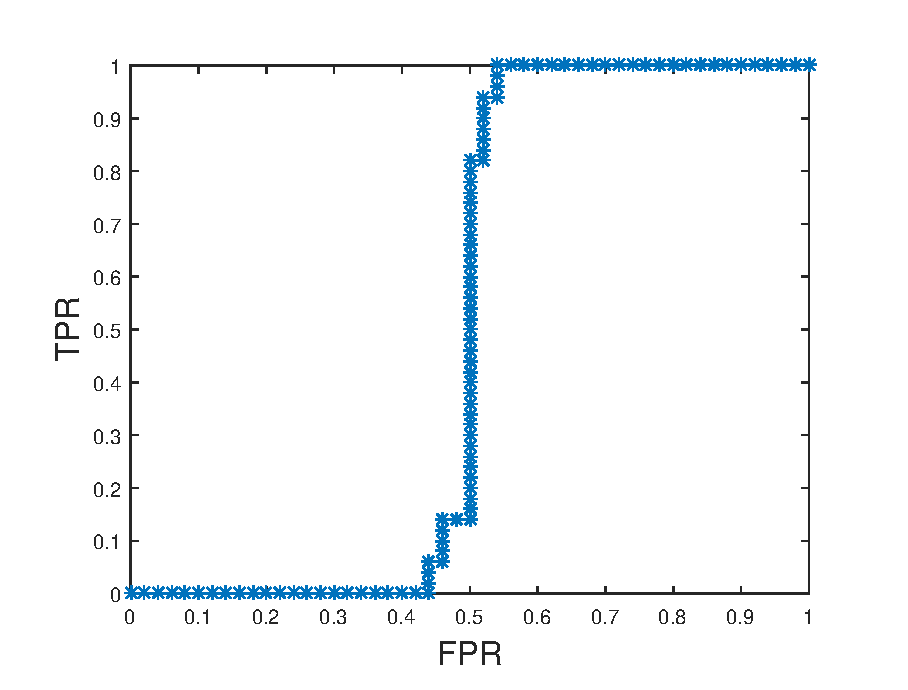
\includegraphics[width=0.6\textwidth]{figuras/prueba.eps}
	\caption{Pie de figura. Poner aquí cita del lugar de donde 
	se ha tomado la imagen en caso de que sea así. }
	\label{fig:prueba}
\end{figure}
\end{verbatim}

% Y ahora pongo la plantilla para que se incluya la figura efectivamente
\begin{figure}[t]
	\centering
	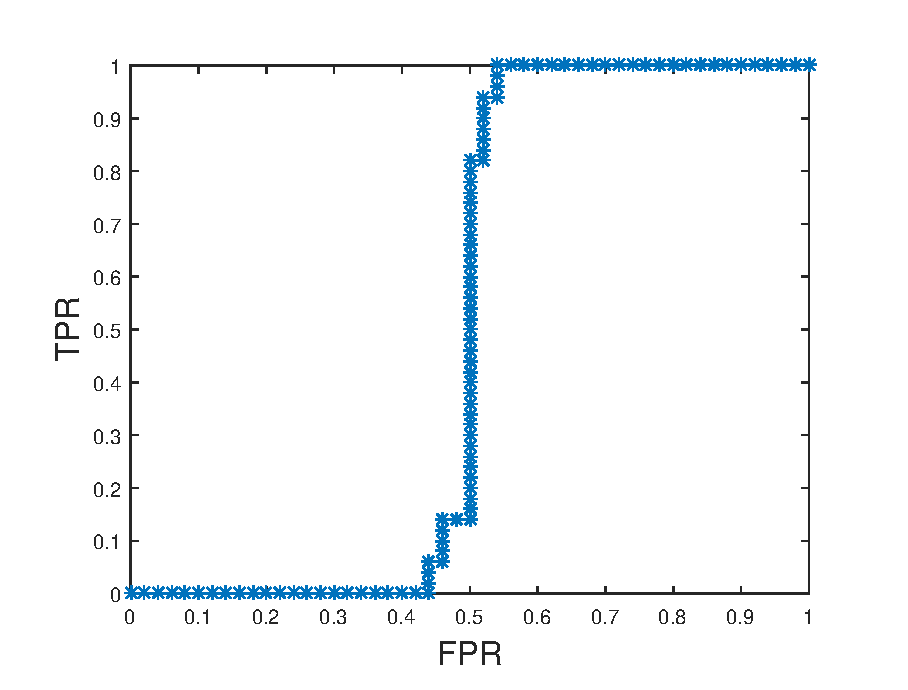
\includegraphics[width=0.6\textwidth]{figuras/prueba.eps}
	\caption{Pie de figura. Poner aquí cita del lugar de donde se ha tomado la imagen en caso de que sea así. }
	\label{fig:prueba}
\end{figure}

Si se pone el modificador [t] (top) latex ubicará la figura en la parte de arriba de la página. Ver otros modificadores como [h] (here) o [b] (bottom). Se pueden usar otras plantillas para, por ejemplo, poner dos figuras una al lado de otra. Consultar en Internet diferentes plantillas en caso de necesidad. 

Cuando en el texto nos refiramos a la figura en cuestión por el número, debemos usar la mayúscula y utilizar referencia a la figura. Esto hará que no nos tengamos que preocupar de la numeración de las figuras. Ej. Como se puede comprobar en la Figura~\ref{fig:prueba}.

Sustituir expresiones del tipo: “En la siguiente figura…” por “En la Figura 2.2…”


\subsection*{Inserción de tablas}

Este sería un ejemplo de una tabla. Se puede modificar el formato y contenido (ver en Internet algún enlace sobre cómo formatear tablas en latex). 

\begin{table}[t]
	\caption{Descripción de la tabla.}
	\label{table:prueba}
	\centering
	\begin{tabular}{l  c} 
		\hline \\[-1.5ex]
		\textbf{Tipo de ataque} & \textbf{Etiqueta} \\ [1ex] 
		\hline\hline \\[-1.5ex]
		DoS11 & dos \\ [0.5ex]
		Exf1MBp & exf1KB \\ [1ex]
		\hline
	\end{tabular}
\end{table}

La forma de referirse a las tablas es similar a las de las figuras (usar mayúsculas y referencia a la etiqueta(label) de la tabla). Ej. Como se puede ver en la Tabla~\ref{table:prueba}, ...


\subsection*{Citas de bibliografía}
Ejemplo de cita de bibliografía. Primero se va a google.scholar y se busca la referencia. Después se da al enlace citar, y se elige el formato bibtex. Se copia ese texto en el fichero bibliografia.bib. Un ejemplo de referenciar una cita es \cite{macia2008evaluation}.


\subsection*{Referencias a secciones}

Para referirnos a secciones, primero debemos tener una etiqueta de tipo \texttt{label} en dicha sección. Posteriormente, pondremos una referencia a dicho label, igual que hacemos para las figuras y las tablas. Ej. Como se ha mencionado en la Sección~\ref{sec:intro:motivacion} (Nótese que la palabra Sección va con mayúscula).

\subsection*{Glosario y acrónimos}

Cuando se utilice un acrónimo se debe definir en el fichero glosario/entradas\_glosario, tal y como está el ejemplo en dicho fichero. Al referirse en el texto se indicará así: \gls{svm} (ver que la primera vez lo pondrá completo). La segunda vez que se referencie a \gls{svm} ya no aparece completo. También se puede nombrar en plural así: \glspl{svm}. 
Otros ejemplos de acrónimo son: \gls{gcd}, \gls{lcm}, \gls{gmf}. 

A la hora de compilar con el glosario, se debe abrir una terminal CMD en el directorio de los fuentes latex del proyecto, y ejecutar el siguiente comando: \texttt{makeglossaries proyecto}. Esto generará los ficheros auxiliares que contienen el glosario. 

\subsection*{Listados de código}

Aquí se puede ver un ejemplo de listado de código: 

%\begin{lstlisting}[frame=none, numbers=none]


\begin{lstlisting}[language=Python,caption=Ejemplo de Python, label=listado:pythonPrueba]
import numpy as np

def incmatrix(genl1,genl2):
	m = len(genl1)
	n = len(genl2)
	M = None #to become the incidence matrix
	VT = np.zeros((n*m,1), int)  #dummy variable

	#compute the bitwise xor matrix
	M1 = bitxormatrix(genl1)
	M2 = np.triu(bitxormatrix(genl2),1) 
	
	for i in range(m-1):
		for j in range(i+1, m):
			[r,c] = np.where(M2 == M1[i,j])
			for k in range(len(r)):
				VT[(i)*n + r[k]] = 1;
				VT[(i)*n + c[k]] = 1;
				VT[(j)*n + r[k]] = 1;
				VT[(j)*n + c[k]] = 1;
	
	if M is None:
		M = np.copy(VT)
	else:
		M = np.concatenate((M, VT), 1)
	
	VT = np.zeros((n*m,1), int)
	
	return M

\end{lstlisting}

Nos podemos referir a él como Listado de código~\ref{listado:pythonPrueba}. 
Si queremos que aparezca como un flotante en la página debemos poner la palabra \texttt{float} así: 
\begin{verbatim}
\begin{lstlisting}[float,language=Python,caption=Ejemplo de Python, 
label=listado:pythonPrueba]
\end{verbatim}


\subsection*{Enlaces URL}
Podemos poner un enlace así \url{http://dtstc.ugr.es/~gmacia}
	\chapter{Introducción}

El objetivo de este proyecto es evitar que un sistema \textit{blockchain} sea vulnerable a futuros ataques cuánticos. Para ello se ha implementado un algoritmo criptográfico resistente a ordenadores cuánticos, denominado UOV, para la firma de documentos, y posteriormente integrarlo en la \textit{blockchain} ARK.

\section{Motivación y contexto del proyecto}
\label{sec:intro:motivacion} %Esto se pone si queremos hacer referencia a esta sección

%En esta parte es importante clarificar las siguientes preguntas: 
%\begin{enumerate}
%\item ¿Cuál es el problema que pretendemos resolver con este proyecto? Debemos introducir un poco el contexto en el que aparece y describir bien en qué consiste dicho problema. 
%\item ¿Por qué es importante dicho problema? Hay que tratar de aportar datos y argumentos para indicar que el problema descrito es relevante en el contexto actual. 
%\end{enumerate}

La tecnología ha transformado nuestra sociedad en una sociedad digitalizada, donde actualmente, los dispositivos digitales comportan la mayor parte de nuestras actividades diarias en distintos ámbitos, como económicas, organizativas o sociales. En el proceso de digitalización de la sociedad podemos distinguir las siguientes cinco fases \cite{fases-digitalizacion}.\\

La primera fase o era del Internet, corresponde a mediados de los 90. En esta fase se comenzaron a crear páginas web para que los medios de comunicación y las empresas puedieran publicar y compartir información.

La segunda fase o era de las redes sociales, tuvo mayor auge a partir de 2005. Plataformas de bajo o ningún coste, se utilizaban en las empresas para poder llegar mejor a los clientes.

La tercera fase o era de la economía colaborativa, nació con la crisis de  2008 cuando las empresas tenían pocos recursos. Surgieron plataformas para conectar a las personas, y poder obtener lo que necesitasen unas de otras. Por ejemplo pagos online, ver recomendaciones y reseñas de un alojamiento o pedir un taxi. Además se da un gran paso ya que estas aplicaciones pasan de estar  alojadas en ordenadores a teléfonos inteligentes.

La cuarta fase o era del mundo autónomo, se ha desarrollado durante décadas. Se desarrollan tecnología con inteligencia artificial, es decir, que simulan la inteligencia de los humanos para poder resolver problemas más complejos.

Quinta fase o era del bienestar moderno, comienza con las pulseras inteligentes como \textit{Fitbit} o \textit{Fuelband} de Nike. Estas pulseras son el impulso de la tecnología para facilitar la vida de los clientes y poder integrar la tecnología en la vida de los mismos.\\

La digitalización debe de venir acompañada de mecanismos que aporten seguridad a los datos. Los pilares de la seguridad de la información son los conocidos como la tríada CIA (confidencialidad, integridad y  disponibilidad)\cite{servicios-seguridad}.\\

La \textbf{confidencialidad} es la propiedad que impide que la información pueda ser accesible por entidades no autorizadas. Un sistema garantiza la confidencialidad cuando un tercero entra en posesión de la información intercambiada entre el remitente y el destinatario, no es capaz de extraer ningún contenido legible. Para asegurar la confidencialidad se utilizan mecanismos de cifrado y ocultación de la comunicación.

La \textbf{integridad} busca mantener la exactitud de los datos, es decir, que no hayan sido modificados durante su envío. La integridad se obtiene adjuntando al mensaje otro conjunto de datos de comprobación de la integridad, un ejemplo es la firma digital.

La \textbf{disponibilidad} es la cualidad de la información de encontrarse a disposición de quienes deben acceder a ella, ya sean personas, procesos o aplicaciones, en el momentos que así lo quieran. Los mecanismos para asegurar la disponibilidad se implementan con la infraestructura tecnológica.\\

Además de estos tres pilares hay otro principio, la \textbf{autentificación}, que es la propiedad que permite identificar al generador de la información. Trata de comprobar si un mensaje enviado por un usuario, ha sido verdaderamente firmado por él mismo. Esto se consigue con el uso de cuentas de usuario y contraseñas de acceso.\\

Para garantizar estos servicios de seguridad se hace uso de protocolos de seguridad de la información entre los que se encuentra la criptografía, la lógica y la autenticación.\\

La criptografía se ocupa de cifrar ciertos mensaje con el fin de hacerlos ilegibles a receptores no autorizados, una vez que llega a su destino y sea descifrado, el receptor obtendrá el mensaje original \cite{criptografia}. Además dota de seguridad a las comunicaciones, a la información y a las entidades que se comunican.

Podemos diferenciar dos tipos de criptografía, la criptografía simétrica y la asimétrica. La criptografía simétrica utiliza la misma clave para cifrar y descrifrar un mensaje, esta clave la ha de conocer tanto el emisor como el receptor. Mientras que la asimétrica utiliza dos claves la pública y la privada.

En la criptografía asimétrica podemos diferenciar dos ramas, el cifrado de clave pública y las firmas digitales \cite{criptografia-asimetrica}. En el cifrado de clave pública, el emisor cifra el mensaje con la clave pública del destinatario y el receptor lo descifra con su propia clave privada. En las firmas digitales, el emisor firma el mensaje con su clave privada y el receptor puede verificar el mensaje con su propia clave pública, además cualquier manipulación del mensaje se refleja en su resumen o \textit{hash}.\\

Este tipo de criptografía basa su seguridad en la hipótesis de que no se pueden encontrar las claves por fuerza bruta con la tecnología existente en la actualidad. Los ataque de fuerza bruta tratan de recuperar las claves probando todas las posibles combinaciones hasta encontrar la que permite el acceso, a partir del algoritmo de cifrado y del texto cifrado con su original \cite{fuerza-bruta}. Para que la búsqueda tenga éxito se deberán de realizar $10^n-1$ operaciones donde $n$ es la longitud de la clave. 

Otro factor importante, en la seguridad, es si en la clave aparencen números, caracteres o la combinación de ambos, aumentando así el coste de encontrar las claves, llegando a alcanzar tiempos de cálculo logarítmicos, es decir, que podrían tardar siglos en encontrar una contraseña compleja pero también depende de la capacidad de operación del ordenador.\\

En este contexto, la aparición de la futura computación cuántica permitirá el cálculo de operaciones a una velocidad mucho mayor. En la gráfica \ref{fig:comp-clasica-cuantica} podemos observar la capacidad de cómputo del peor ordenador cuántico, con la línea continua, que sigue la gráfica de una función exponencial, frente a la capacidad del mejor ordenador clásico, la línea discontinua, que sigue una función lineal.

\begin{figure}[h]
	\centering
	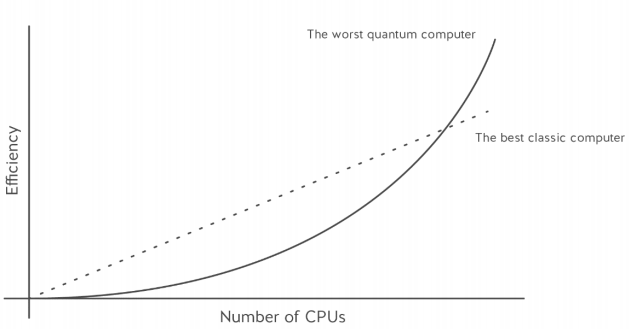
\includegraphics[width=0.8\textwidth]{figuras/comp_clasica_cuantica.png}
	\caption{Comparativa de la capacidad de cómputo de un ordenador clásico con un ordenador cuántico\cite{clasica-vs-cuantica}}
	\label{fig:comp-clasica-cuantica}
\end{figure}

La comparativa también nos muestra que para operaciones pequeñas como, por ejemplo, editar un documento de texto un ordenador cuántico sería probablemente ineficienciente. Por tanto lo mejor sería un ordenador híbrido, que mezclase computación clásica, para cálculos pequeños, y computación cuántica, para operaciones de mayor tamaño.\\

Cuando esté desarrollado el ordenador cuántico no serán válidos los actuales algoritmos criptográficos de clave pública, como \acrshort{rsa}, Diffie-Hellman y \mbox{\acrshort{ecdsa}}, ya que se basan en los problemas del logaritmo discreto y factorización de enteros, resolubles fácilmente por un ordenador cuántico. Las primeras ideas de la criptografía cuántica se tiene en los años 70, destacando los algoritmos de Shor y Grover.

Veamos la tabla comparativa \ref{table:security-level}, esta nos indica el tipo de algoritmo criptográfico, el algoritmo con la longitud de la clave y a continuación el nivel de seguridad tanto en un ordenador clásico como en uno cuántico. El nivel de seguridad de un algoritmo nos indica el número de operaciones necesarias para romper dicho algoritmo, por ejemplo, si tiene un nivel de seguridad $n$ entonces se requieren $2^n$ operaciones para romper el algoritmo \cite{security-level}. Observamos que hay una diferencia considerable en los niveles de seguridad de los algoritmo asimétricos, puesto que con un ordenador clásico al menos se necesitan $2^{112}$ operaciones mientras que con computación cuántica solo una. \\

\begin{table}[h]
	
	
	\centering
	\resizebox{\linewidth}{!}{
	\begin{tabular}{c c c c c }
		\hline \\[-1.5ex]
		\thead{Tipo} & \thead{Algoritmo-Longitud clave} & \thead{Nivel seguridad\\ (ordenador clásico)} & \thead{Nivel seguridad\\ (ordenador cuántico)} & \thead{Ataque cuántico}\\ [1ex] 
		\hline\hline \\[-1.5ex]
		\multirow{4}{5em}{Asimétrico} & RSA-2048 & 112 & 0 & Algoritmo de Shor \\ [0.5ex]
		& RSA-3072 & 128 & 0 & Algoritmo de Shor \\ [0.5ex]
		& ECC-521 & 128 & 0 & Algoritmo de Shor \\ [0.5ex]
		& ECC-521 & 256 & 0 & Algoritmo de Shor \\ [0.5ex]
		\hline \\[-1.5ex]
		\multirow{2}{5em}{Simétrico} & AES-128 & 128 & 64 & Algoritmo de Grover \\ [0.5ex]
		& AES-256 & 256 & 128 & Algoritmo de Grover \\ [1ex]
		\hline
	\end{tabular}}
	\caption{Niveles de seguridad de ordenadores clásicos y cuánticos \cite{security-bit}}
	\label{table:security-level}
\end{table}


En la actualidad, se están desarrollando muchos algoritmos para que sean resistentes a ataques de tipo cuántico, denominados algoritmos de criptografía postcuántica \cite{criptografia-postcuantica}. Estos ataques afectan principalmente a los algoritmos de clave pública o asimétrica, puesto que para la criptografía simétrica duplicar el tamaño de clave empleada es suficiente para hacerlos seguros y hacer inservible el algoritmo de Grover.\\

Por otro lado, también en la actualidad está siendo muy relevante la adopción de las \textit{blockchain} como tecnología para ofrecer diversos servicios. Las \textit{blockchain} o cadenas de bloques son listas de transacciones, denominadas bloques, firmadas y unidas con algoritmos criptográficos. Además cada bloque contiene el hash del bloque anterior, se explicará con más detalle en la sección \ref{sec:intro:blockchain}. 

Esta tecnología se ha integrado en diferentes áreas, donde resalta el uso en los servicios financieros o criptomonedas, que aumenta la eficiencia y disminuye los costes. Otro uso de las \textit{blockchain} es en las cadenas de suministro, algunos restaurantes, como Fogo de Ch\~{a}o \cite{Fogo-Chao}, están empezando a utilizar las \textit{blockchain} para poder rastrear el origen de sus alimentos hasta llegar al propio restaurante, una gran ventaja para encontrar fácilmente si hay algún producto contaminado o en mal estado. \\

Un ejemplo del uso de las \textit{blockchain} queda reflejado en este proyecto en el que se ha implementado un algoritmo resistente a ataques cuánticos, UOV \cite{algoritmo-UOV} y se ha adaptado a la \textit{blockchain} ARK \cite{ark} para que se utilice dicho algoritmo de firma.\\


\section{Objetivos del proyecto y logros conseguidos}
\label{sec:intro:objetivos}
El objetivo de este proyecto es modificar el algoritmo de firma y verificación de las transacciones de la \textit{blockchain} ARK, para hacerla resistente a ataques cuánticos.

\begin{itemize}
	\item Implementación del algoritmo UOV: Se ha implementado las funciones de generación de claves tanto públicas como privadas, la función de firma a partir de la clave privada y la función de verificación de la misma con la clave pública. Además ha sido necesario implementar la aritmética de cuerpo finito de $2^7$ elementos.
	\item Integrar el algoritmo UOV en la \textit{blockchain} ARK para comprobar su funcionamiento: Se ha modificado el algoritmo de firma dado en la \textit{blockchain} por el algoritmo UOV para aumentar la seguridad.

\end{itemize}


\section{Estructura de la memoria}
%Se describirán los capítulos que tiene la memoria, indicando qué contenidos habrá en cada uno de ellos, para permitir al lector situarse ante el documento. 

A continuación se muestran los capítulos que presenta la memoria junto con una breve descripción de lo que contiene cada uno.

\begin{enumerate}
	\item Introducción: Presenta la motivación del proyecto y el contexto en el que surge, además incluye una breve reseña introduciendo las dos tecnologías que se han utilizado computación cuántica y la \textit{blockchain}, aparte de la explicación matemática del algoritmo utilizado. En este capitulo también se encuentran los objetivos que se persiguen con este trabajo.
	\item Planificación y costes: Contiene el diagrama de Gantt con la defición de las entregas y seguimiento del proyecto, así como el presupuesto del proyecto.
	\item Análisis del problema: Descripción de las funcionalidades y requisitos, y análisis de los objetivos que se muestran en la sección \ref{sec:intro:objetivos}.
	\item Diseño: Se encuentra el diseño de la implementación del algoritmo UOV y el diseño del ecosistema ARK, donde se integrará el algoritmo de firma.
	\item Implementación: Contiene la explicación de la implementación del algoritmo UOV y la aritemética del cuerpo finito de $2^7$ elementos.
	\item Evaluación y pruebas: Ejemplo de la firma de una transacción en el sistema ARK.
	\item Conclusiones
\end{enumerate}

\section{Contenidos teóricos para la comprensión del proyecto}

En los siguientes apartados se explica los contenidos claves de este proyecto, que son la computación cuántica\ \ref{sec:intro:cc}, la tecnología \textit{blockchain}\ \ref{sec:intro:blockchain} y el algoritmo UOV\ \ref{sec:intro:UOV}.

\subsection{Computación cuántica}\label{sec:intro:cc}

La evolución de la tecnología se ha basado principalmente en la reducción de los transistores para aumentar la velocidad, llegando a escalas de tan solo algunas decenas de nanómetros. Esto tiene un límite y es la eficiencia, puesto que al seguir disminuyendo el tamaño podrían dejar de funcionar correctamente. De ahí surge la necesidad de descubrir nuevas tecnologías, la computación cuántica \cite{computacion-cuantica-wiki}. Así la computación cuántica constituye un nuevo paradigma de la informática basado en los principios de la teoría cuántica.\\

Las tecnologías cuánticas nacieron del estudio de algunos fenómenos físicos que aún no se entendían bien, entre los años 1900 y 1930, dando lugar a una nueva teoría en la física, la Mecánica Cuántica. La Mecánica Cuántica es la rama de la física que estudia del mundo microscópico, los sistemas atómicos y subatómicos y su interacción con la radiación electromagnética \cite{mecanica-cuantica}.\\

\subsubsection{Historia}

La computación cuántica tuvo sus inicios en los años 50 cuando algunos físicos, como Richard Feynman, fueron pioneros en mencionar posibilidad de utilizar efectos cuánticos para realizar cálculos computacionales \cite{computacion-cuantica-wiki}. En la charla de Richard Feynman titulada ``Simulación de la física con computadoras'', a principio de la década de los 80, expuso algunos cálculos complejos que se podrían realizar más rápido con un ordenador cuántico. 


A finales de los años 60, Stephen Wiesner escribe un artículo titulado ``Conjuate Coding'', donde expone un primer acercamiento a la criptografía cuántica, el artículo fue publicado en los años 80 \cite{computacion-cuantica-crono}.

En 1981 Paul Benioff expone las ideas esenciales de la computación cuántica acompañada de su teoría, en la que propuso que un ordenador clásico trabajara con algunos pricipios de la mecánica cuántica, y aprovechar así las leyes cuánticas.\\


En la década de 1990 ya empezaron a poner en práctica algunas teorías, apareciendo los primeros algoritmo cuántidos, primeras aplicacines cuánticas y las primeras máquinas diseñadas para realizar cálculos cuánticos. Así en 1991, Artur Ekert desarrolla una aproximación diferente a la distribución de claves cuántica (QKD) basado en el entrelazamiento cuántico.

En 1993 hubo varios acontecimientos, por un lado, Dan Simon comparó el modelo de probabilidad clásica con el cuántico, esto se utilizó para el desarrollo de futuros algoritmos cuánticos. Por otro, Charles Benett acuñó el término del teletransporte cuántico, abriendo una vía de investigación para las comunicaciones cuánticas. Además Ekert organizó la primera conferencia internacional de criptografía cuántica en Inglaterra, primer evento de gran alcance dedicado a este área.

Peter W. Shor definió un algoritmo cuántico, el algoritmo de Shor, que permite calcular los factores primos de números muy grandes en tiempo polinimial, resolviendo el problema de la factorización de enteros como el problema del logaritmo discreto. Como consecuencia, el algoritmo de Shor permite romper muchos sitemas criptográficos actuales. Un año más tarde, propuso un sistema de corrección de errores en el cálculo cuántico.

Lov Grover, en 1996, expone un algoritmo de búsqueda en una secuencia de datos no ordenada con N elementos, denominado algoritmo de Grover, que tiene una complejidad en tiempo de $O(\sqrt{n})$.

En 1997, tiene lugar el primer experiemento de comunicación con criptografía cuántica a una distancia de 23km. Además del primer teletransporte cuántico de un fotón.

A finales de los 90, los laboratorios IBM-Almaden crearon la primera máquina con 3 cúbits y ejecutó el algoritmo de Grover. Y en 2001, IBM junto con la Universidad de Stanford ejecutaron el algoritmo de Shor en un computador cuántico con 7 cúbits, se calcularon los factores primos de 15.\\

En 2004, sale a la luz el primer criptosistema cuántico comercial(QKD), creado por la ID Quantique.

En 2007, D-Wave fabricó una máquina que utilizaba mecánica cuántica con 16 cúbits sin llegar a ser un computador cuántico, especializado en la optimización de problemas a través de algoritmo de temple cuántico. En septiembre de ese mismo año, consiguieron unir componentes cuánticos a través de superconductores, apareciendo el primer bus cuántico capaz de reter información cuántica durante un corte espacio de tiempo antes de volver a ser transferida. Un año después se consiguió almacenar un cúbit en el interior del núcleo de un átomo de fósforo y hacer que la información permaneciera intacta durante 1.75 segundos.

Pasaron varios años hasta que se vendió la primera computadora cuántica comercial, en 2011, por la empresa D-Wave Systems por 10 millones de dólares.

En 2018, la Universidad de Innsbruck consiguen un entrelazamiento estable de 20 cúbits, marcando el récord actual. El 18 de septiembre de 2019, IBM anunción que pronto lanzará un ordenador cuántico de 53 cúbits, el más grande y potente hasta la fecha.\\

En la actualidad, Google ha logrado aplicar una supercomputadores al mundo real, simulando con éxito una reacción química simple. Marcando el camino hacia la química cuántica. Esto podría ayudar a los científicos a comprender mejor las reacciones moleculares, dando lugar a descubrimientos útiles como mejores baterías, nuevas formas de producir fertilizante y métodos para eliminar el dióxido de carbono del aire \cite{quimica-cuantica}.

\subsubsection{Estructura de los cúbits}

La computación clásica funciona con bits cuyos valores pueden ser 0 o 1, mientras que la computación cuántica funciona con bit cuánticos o cúbits, una combinación de 0 y 1, pudiendo tomar ambos valores a la vez, esto se denomina la superposición cuántica de los estados \cite{computacion-cuantica-criptografia}, se entrará en detalle más adelante.

La figura \ref{fig:bit-cubit} muestra los estados de un bit y los posibles estados que puede tomar un cúbit. 

\begin{figure}[h]
	\centering
	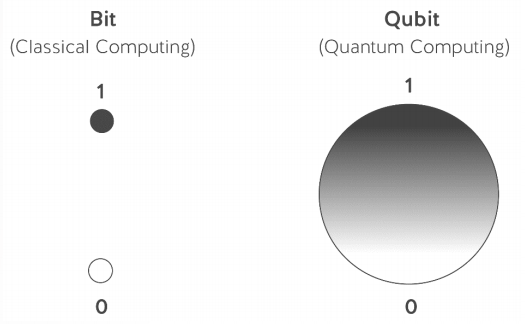
\includegraphics[width=0.8\textwidth]{figuras/bit_cubit.png}
	\caption{Estados de un bit y de cúbit \cite{clasica-vs-cuantica}}
	\label{fig:bit-cubit}
\end{figure}

El espacio de estados de un cúbit se puede representar mediante un espacio vectorial complejo bidimensional, al no ser práctico, se aprovecha el homeomorfismo entre la superficie de una esfera y el plano complejo cerrado con un punto en el infinito, dando lugar a lo que se conoce como la esfera de Bloch.  

Una esfera de Bloch es una representación geométrica del espacio de estados puros de un sistema cuántico de dos niveles. Además se representa en el espacio $\mathds{R}^3$ por la esfera de radio unidad como se observa en la imagen \ref{fig:esfera-bloch}, donde cada punto de la esfera es un posible estado del cúbit. 


\begin{figure}[h]
	\centering
	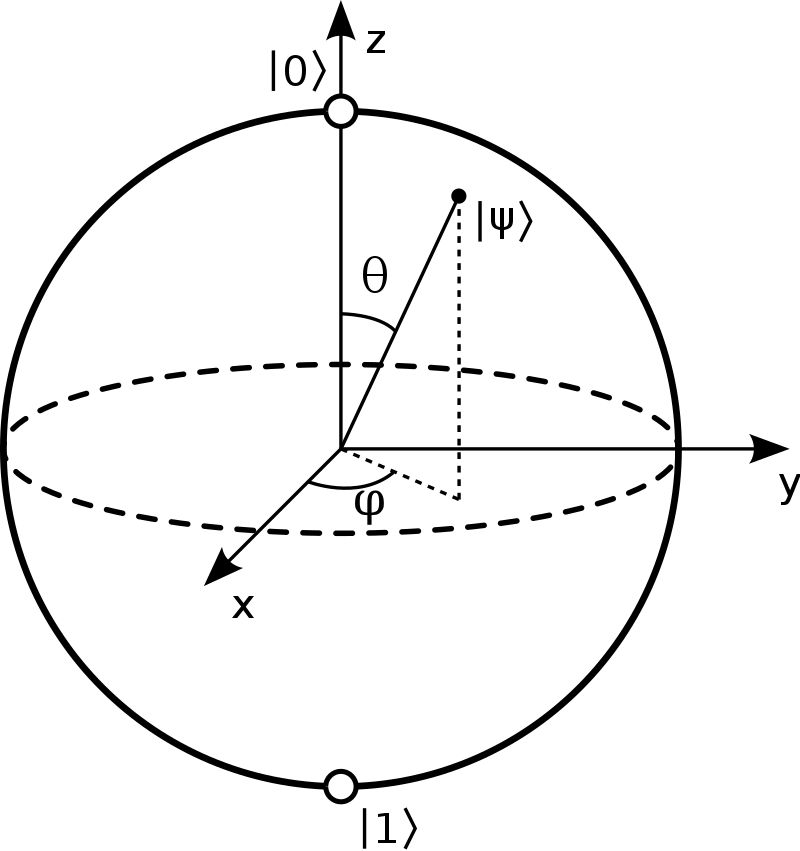
\includegraphics[width=0.4\textwidth]{figuras/esfera_bloch.png}
	\caption{Estructura cúbit, esfera de Bloch \cite{esfera-bloch}}
	\label{fig:esfera-bloch}
\end{figure}

Un cúbit se puede representar como una combinación lineal de los estados $|0\rangle$ y $|1\rangle$, ecuación \ref{eq:cubit}.

\begin{equation}\label{eq:cubit}
|\psi \rangle = \alpha|0\rangle + \beta |1\rangle
\end{equation}

Como $\alpha$ y $\beta$ son números complejos, la ecuación \ref{eq:cubit} se puede escribir en forma exponencial, ecuación \ref{eq:cubit-expo}.

\begin{equation}\label{eq:cubit-expo}
|\psi\rangle = r_{\alpha} e^{i\phi_{\alpha}}|0\rangle + r_{\beta} e^{i\phi_{\beta}}|1\rangle\\
\end{equation}

\vspace{1em}
\subsubsection{Propiedades}
Entre las propiedades cuánticas destacan la superposición cuántica, el entrelazamiento cuántico y el teletransporte cuántico.\\

La \textbf{superposición cuántica} describe cómo una partícula puede estar en diferentes estados al mismo tiempo. Esto aporta gran capacidad de procesamiento, lo que hace posible resolver de manera eficiente problemas de mayor complejidad como la factorización de enteros, el algoritmo discreto y la simulación cuántica, que a día de hoy con los ordenadores clásicos son difíciles de romper. 

Otro aspecto importante de la física cuántica relacionado con la superposición es el \textbf{entrelazamiento cuántico} de las partículas\cite{cumputacion-cuantica-clasica}. Esto es, si dos partículas en algún instante han interactuado retienen un tipo de conexión y pueden entrelazarse formando pares, de forma que al interacturar con una de las particulas, por muy separadas que estén, la otra se entera. Esto permite que aunque los cúbits estén separados interactúen entre sí. Con estos dos aspectos la capacidad de procesamiento aumenta considerablemente, cuántos más cúbits la capacidad de procesamiento aumenta considerablemente.

Por último, el \textbf{teletransporte cuántico} utiliza el entrelazamiento para enviar información de un lugar del espacio a otro sin necesidad de viajar a través de él.




\subsection{Blockchain}\label{sec:intro:blockchain}


\textit{Blockchain} es un sistemas de almacenamiento de información que se divide en bloque de datos enlazados mediante los hash. A cada bloque se le asocia un hash a partir del bloque anterior, creando una lista enlazada, la búsqueda de información no es muy óptima si hay un número elevado de bloques. Para la búsqueda eficiente en \textit{blockchain} se usan los árboles merkle.\\

Los datos que almacena cada bloque son transacciones válidas, información referente a ese bloque y la relación con el bloque anterior mediante el \textit{hash}, por tanto el bloque tiene un lugar específico dentro de la cadena. De esta forma si hay una alteración en un determinado bloque se verá reflejado en su \textit{hash} y en el de los bloques posteriores, haciendo que la información de la cadena no se pueda perder, modificar o eliminar.\\


Los árboles merkle \cite{arbol-merkle} son una estructura de datos en árbol en el que cada nodo que no es hoja está etiquetado con el \textit{hash} que surge de la combinación de los valores o etiquetas de sus nodos hijo. Esta estructura permite que aunque los datos estén separados puedan ser ligados a un único valor de \textit{hash}, el \textit{hash} del nodo raíz del árbol. El \textit{hash} de este nodo va firmado para asegurar la integridad y hacer que la verificación sea fiable. 

De esta forma se asegura que los datos son recibidos sin daños y sin ser alterados, además permite que los datos puedan ser entregados por partes, ya que un nodo puede obtener solo la cabecera de un bloque desde una fuente y otra pequeña parte del árbol desde otra fuente, y poder asegurar que los datos son correctos. Esto funciona porque si un usuario intenta hacer un cambio en una transacción falsa en la parte inferior del árbol en seguida se verá reflejado en la parte superior del árbol, es decir, en el nodo raíz. Esta propiedad se ve clara en la estructura del árbol Merkle \ref{fig:arbol-Merkle}, donde los \textit{hash} de los nodos superiores se calculan a partir de los \textit{hash} de los nodos hijos.\\

\begin{figure}[h]
	\centering
	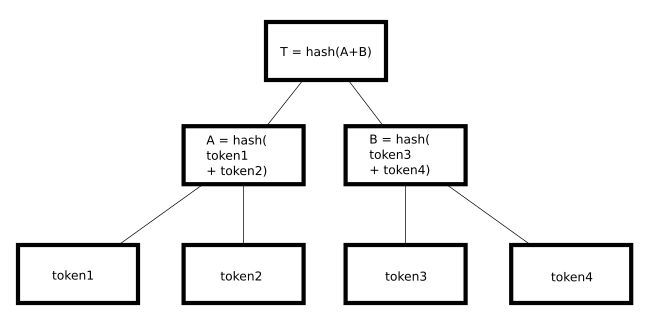
\includegraphics[width=0.8\textwidth]{figuras/arbol_merkle.png}
	\caption{Estructura de un árbol Merkle \cite{img-arbol-merkle}}
	\label{fig:arbol-Merkle}
\end{figure}

La idea de la tecnología \textit{blockchain} surge a comienzos de 1991 cuando los científicos Stuart Haber y W. Scott Stornetta introducen una solución computacional para la firma de documentos digitales y que no puedieran ser modificados con el tiempo. Usaron cadenas de bloque para almecenar los documentos con sello de tiempo y en 1992 se incorporaron los árboles Merkle, que podían recopilar varios documentos en un bloque haciendo el diseño más eficiente. Sin embargo, esta tecnología no se utilizó y la patente caducó en 2004 \cite{historia1-block}.

En 1998, Nick Szabo trabaja en una moneda digital descentralizada, ``bit gold''. Dos años después Stefan Konst publica su teoría sobre la seguridad criptográfica en las cadenas de bloques junto con algunas ideas de implementación \cite{historia2-block}.

En 2004, el informático y criptógrafo Harold Thomas Finney introdujo el sistema RPoW (prueba de trabajo reutilizable). El sistema se basa en \textit{HashCash} pero los token de prueba no están ligados a una aplicación sino que pueden ser gastados libremente como una moneda. Los clientes pueden crear tokens e intercambiarlos sin necesidad de regenerarlos \cite{RPoW}. RPoW resolvió el problema del doble gasto registrando los tokens en un servidor fiable diseñado para permitir a los usuarios verificar su exactitud e integridad en tiempo real. Este sistema puede considerarse como un prototipo de las criptomonedas.

A finales de 2008, un grupo de desarrolladores bajo el nombre de Satoshi Nakamoto publican un documento técnico en que se establece un modelo para \textit{blockchain}. Está basado en el algoritmo RPoW pero en lugar de usar dicho hardware, se utiliza un protocolo descentralizado peer-to-peer para verificar y restrear las transacciones. En otras palablas los ``mineros'' extraen bitcoins para obtener una recompensa mediantes pruebas de trabajo y posteriormente los nodos los verifican. Bitcoin nació el 3 de enero de 2009 cuando Satoshi Nakamoto extrajo el primer bloque de bitcoin con una recompensa de 50 bitcoins. Y el 12 de enero de 2009 tuvo lugar la primera transacción entre Satoshi Nakamoto y Hal Finney que obtuvo 10 bitcoins.

A partir de 2014, se comienzan a explorar el potencial de las cadenas de bloque y a buscar otras aplicaciones fuera de su uso en las transacciones financieras.
Ethereum introduce programas informáticos que se ejecutan en la \textit{blockchain}, se pueden utilizar para realizar una transacción cumpliendo ciertas condiciones como los contratos inteligentes.

Un contrato inteligenete se tratan de contratos que tienen la capacidad de cumplirse de forma automática. Un contrato inteligente está constituido por un protocolo de códigos que permiten a un dispositivo ejecutar de forma automatizada las sentencias previamente programadas, prescindiendo de la intervención humana \cite{contrato-inteligente}.

Además de los contratos inteligentes, Ethereum tiene su propia criptomoneda llamada Ether, se puede transferir entre cuentas y se utiliza para pagar las tarifas por la ejecución de los contratos inteligentes.

Actualmente las \textit{blockchain} tiene otros usos más allá de las criptomonedas.\\


Las cadenas de bloques o \textit{blockchain} permiten verificar, validar, rastrear todo tipo de información, ya sean contratos inteligentes, transacciones financieras, certificados digitales o firmas \cite{blockchain}, siendo estas últimas el centro de este trabajo. También permiten impulsar modificaciones orientadas a crear soluciones más robustas, por ejemplo en centros de salud o notarías que se explicarán más adelante.\\

Las \textit{blockchain} son vulnerables a futuros ataques cuánticos ya que su única línea de defensa es el algoritmo de firma de los bloques. Aunque, actualmente las cadenas de bloques son seguras, puesto que un ordenador clásico no tiene la capacidad de cómputo necesaria para descifrar cada bloque, obtener la información y volver a firmar todos los bloques sin dejar huella. Por eso para hacer una \textit{blockchain} resistente es necesario tener un criptosistema que no se pueda romper con computación cuántica, como por ejemplo el algoritmo UOV, ver apartado \ref{sec:intro:UOV}. \\

Los tres pilares de la tecnología \textit{blockchain} son la descentralización, transparencia e inmutabilidad \cite{pilares-blockchain}.

Un sistema centralizado almacena todos los datos en una misma entidad y habría que interactuar con la misma para obtener la información necesaria. Un ejemplo de un sistema centralizado son los bancos que almacenan todo el dinero y la única forma de pagar a alguien es a través de un banco. Es similar a la arquitectura cliente-servidor donde los clientes se comunican entre ellos mediante el servidor. Pero tener un único sitio para almacenar todos los datos es vulnerable a los ataques, informáticos, por otra parte si el nodo central se corrompe o tiene una actualización, los datos será incorrectos o no se podrán acceder a ellos. De los contras de los sistemas centralizados surge la idea de los sistemas \textbf{descentralizados}, la información no la tiene un único nodo sino que todos los usuarios son dueños de la información. La principal ideología de las \textit{blockchain} es poder interactuar usuario con usuario sin tener que pasar por un tercero.

El concepto \textbf{transparencia} se refiere a la transparencia de los datos no de las identidades. Esto es la identidad de la persona se oculta a través de la criptografía y lo único que se ve es su dirección pública, pero podemos ver todas las transacciones que se han realizado en su dirección pública. En el historial de transacciones no vemos ``Antonio envió 1BTC'' sino que aparece ``\sloppy{1MF1bhsFLkBzzz9vpFYEmvwT2TbyCt7NZJ} envió un 1BTC''. Este nivel de transparencia nunca antes había existido en el sistema financiero, lo que exige más responsabilidad a las grandes empresas. De la misma forma podemos trasladar este concepto fuera del sistema financiero por ejemplo a las cadenas de suministro, y saber exactamente de donde provienen los alimentos de un restaurante.

La \textbf{inmutabilidad} en el contexto de las cadenas de bloques significa que una vez introducida una transacción en la \textit{blockchain} ya no se puede alterar. De esta forma aplicando esta tecnología a los bancos se evitarían casos de malversación de fondos. Esta propiedad se obtiene gracias a la función criptográfica \textit{hash}.

La función \textit{hash} es el resultado de aplicar una función que transforma un mensaje de longitud variable en uno de longitud fija. Esto es calcular el resto módulo $n$ con $n$ la longitud fija. Al aplicar la función hash a un fichero, si se modifica algún dato del mismo cambiará su hash y por tanto se sabrá si ha sido manipulado desde que se envió, consiguiendo la integridad del mensaje.

De la misma forma si hay un cambio en una de las transacciones de un bloque se reflejará en el \textit{hash} del bloque, afectado a todos los bloques anteriores. Así si el atacante quiere preservar la integridad deberá de modificar todos los bloques siendo una tarea imposible. De esta forma se obtiene la inmutabilidad de los datos.\\

Hoy en día, la tecnología \textit{blockchain} está ganando mucha atención, no limitandose solo al uso en las criptomonedas. Así las cadenas de bloques tienen diversas aplicaciones entre ellas se encuentra la salud o la firma de documentos en las notarías. En el primer caso, cada centro  de salud podría tener el historial médico de cualquier paciente, de una forma segura y evitando falsificaciones, estos historiales se encontrarían en nodos distribuidos de forma descentralizada así se obtendría un acceso rápido y seguro. El segundo caso será en el que nos centraremos a lo largo de este proyecto. Hoy día la firma de documentos o transacciones por parte de un usuario es un problema puesto que se pueden copiar con facilidad, pero con \textit{blockchain} no podrían ser falsificadas debido a la propiedad de validación y rastreo de los datos.\\


\subsection{Algoritmo UOV}\label{sec:intro:UOV}

El algoritmo aceite y vinagre desequilibrado es una versión simplificada del algoritmo aceite y vinagre, ambos algoritmos de firma digital. Para crear las firmas y validarlas es necesario resolver un sistema con $m$ ecuaciones y $n$ variables, que es un problema NP-duro, lo que significa que si fuésemos capaces de resolverlo con un ordenador cuántico, todos los problemas considerados en la actualidad serían vulnerables. Si $m$ y $n$ son casi iguales o iguales será más difícil resolver el sistema, obteniendo de esta forma un algoritmo de firma resistente a ataques cuánticos.\\

La principal ventaja del algoritmo \acrshort{uov} es que es un algoritmo post-cuántico, a diferencia de otros esquemas de firmas como \acrshort{rsa}, \acrshort{dsa}, basado en el logaritmo discreto, y su variante para curvas elípticas \mbox{\acrshort{ecdsa}} que no permanecerían seguros ante un ordenador cuántico. Esto se debe a que en la actualidad no existe un algoritmo eficiente para la resolución de sistemas multivariados de ecuaciones  en ordenador cuántico. Otra ventaja es la simplicidad de las operaciones utilizadas, ya que las firmas se crean y validan con operaciones de suma y multiplicaciones de valores pequeños, lo que requiere bajos recursos \textit{hardware}. 

Aunque el algoritmo usa sistemas pequeños y la longitud de las firmas son pequeñas, se necesitan claves públicas bastante más grandes en comparación con otros algoritmos de firma como \mbox{\acrshort{ecdsa}}, pudiendo ocupar dicha clave pública varios kilobytes de almacenamieno. Por otro lado ya se conocen algunos métodos de ataque, probablemente aparecerán más si se empiza a comercializar.\\

\subsubsection{Cuerpos finitos}
Se trabajará con el cuerpo finito de 128 elementos, $\GF(2^7)$, extensión de grado $7$ del cuerpo $\GF(2)$ de los enteros módulo $2$
 
\begin{equation}
\GF(128) = \frac{\GF(2)[x]}{\langle x^7 + x + 1 \rangle}
\end{equation}

Además el orden del cuerpo de las unidades es $127$, que es primo entonces todo elemento del cuerpo distinto de $1$ es un elemento primitivo, es decir, un generador.\\

La tabla \ref{tab:rel} muestra una representación de los elementos no nulos del cuerpo. En la implementación se ha utilizado la representación como cadena de bits, puesto que a la hora de trabajar es más fácil con una cadeba de bits que con los polinomios.

\begin{table}[h]
	\begin{center}
		\begin{tabular}{p{0.2\linewidth}p {0.2\linewidth}p{0.2\linewidth}}
			\textbf{Polinomio} & \textbf{Bits} & \textbf{$\log_a$}\\
			\toprule
				$1$ & [0, 0, 0, 0, 0, 0, 1] & 0\\
				$a$ & [0, 0, 0, 0, 0, 1, 0] & 1\\
				$a^2$ & [0, 0, 0, 0, 1, 0, 0] & 2\\
				\\
				$\vdots$ & $\vdots$ & $\vdots$\\
				\\
				$a^6 + a^5 + a^4 + 1$ & [1, 1, 1, 0, 0, 0, 1] & 124\\
				$a^6 + a^5 + 1$ & [1, 1, 0, 0, 0, 0, 1] & 125\\
				$a^6 + 1$ & [1, 0, 0, 0, 0, 0, 1] & 126\\
			\bottomrule
		\end{tabular}
	\end{center}
	\caption{Representación de los elementos no nulos de $\GF(128)$}
	\label{tab:rel}
\end{table}

La implementación del cuerpo finito de $2^7$ elementos no se ha realizado de forma genérica sino para que sea específica para el algoritmo UOV, de esta forma es mucho más sencillo implementar la aritmética del cuerpo. Para la suma en $\GF(2)$ sólo tenemos que fijarnos que es lo mismo que el operador lógico \textit{XOR}, mientras que para el producto, al encontrarmos en un cuerpo como un orden pequeño, se usarán unas tablas que contienen las correspondencias entre los elementos no nulos del cuerpo y sus logaritmos en base $a$, por lo que el producto se convierte en una suma módulo $127$.\\




\subsubsection{Parámetros y fórmula}
Para empezar indicamos los parámetros que serán de utilidad para entender el algoritmo.
\begin{itemize}
	\item r: Grado del cuerpo extendido, $\mathds{F}_2 \subset \mathds{F}_{2^r}$. En la implementación se va tomar $r$ igual a $7$, pero se puede realizar con cualquier valor de $r$ sin un esfuerzo adicional.
	\item $m$: Tamaño de la clave pública, además del número de variables de aceite.
	\item $v$: Número de variables vinagre.
	\item $n$: Número total de variables, las de aceite más las de vinagre.
	\item $x$: Vector de $n$ componentes, denominando a las primeras $v$ componentes  $x_1, \dotsb, x_v$ vinagre y al resto aceites.
	
	
	%\item $\mathcal{H}$: Función salida extensible se usa para crear el hash del mensaje y proviene de la clave pública.
	%\item $\mathcal{G}$: Función salida extensible se usa para la generación de la clave pública a partir de una semilla privada.
\end{itemize}

$\mathcal{P}: \mathds{F}_{2^r}^n \rightarrow \mathds{F}_{2^r}^m$, esta función se puede descomponer como $\mathcal{P} = \mathcal{F} \circ \mathcal{T}$, donde $\mathcal{T}: \mathds{F}_{2^r}^n \rightarrow \mathds{F}_{2^r}^n$ es invertible, y $\mathcal{F}: \mathds{F}_{2^r}^n \rightarrow \mathds{F}_{2^r}^m$ siendo sus $m$ componentes de la forma:

\begin{equation}\label{eq:fun}
f_k(x) = \sum_{i=1}^v \sum_{j=i}^n \alpha_{i,j,k} x_i x_j + \sum_{i=1}^n \beta_{i,k} x_i
\end{equation}

donde $\alpha_{i,j,k}$ y $\beta_{i,k}$ se toman aleatoriamente en $\mathds{F}_2$ siendo $\alpha$ un vector de matrices triangulares superiores. De esta manera será más eficiente y no afectará a la seguridad del algoritmo.



\subsubsection{Generación de la clave privada}
La clave privada está formada por $\alpha_{i,j,k}$ y $\beta_{i,k}$ que son valores de $\GF(2)$, elegidos de forma aleatoria.


\subsubsection{Generación de la clave pública}
Generaremos una clave pública partiendo de la clave privada $\alpha_{i,j,k}$ y $\beta_{i,k}$.

Para entenderlo mejor ponemos las $m$ ecuaciones (\ref{eq:fun}) en forma matricial, ecuación \ref{eq:matriz}. La notación a seguir para las matrices transpuestas es $(X)'$, con $X$ una matrix.

\begin{equation}\label{eq:matriz} 
f_k(x) = x^v\ [\alpha_{i,j,k}]\ (x^v, x^m)' + [\beta_{i,k}]\ (x^v, x^m)'
\end{equation}
siendo $[\alpha_{i,j,k}]$ y $[\beta_{i,k}]$ las representaciones matriciales de $\alpha_{i,j,k}$ y $\beta_{i,k}$, $x^v$ los vinagres y $x^m$ los aceites, así $x$ se puede expresar como $(x^v, x^m)'$.\\

Conociendo los valores de la clave privada $\alpha$ y $\beta$, tomando de forma aleatoria los del vinagre $x^v$, los cuales pasaremos a denominarlos como $a^v$, y cogiendo los $m$ primeros bits del hash del mensaje $h_k$ podemos generar la clave pública.

Hacemos el cambio de notación $A_k = a^v\ [\alpha_{i,j,k}] = (A^v_k, A^m_k)$,  lo sustituimos en la ecuación (\ref{eq:matriz}) y despejamos los aceites.

\begin{align}
h_k &= A_k^v\ (a^v)' +  A_k^m\ (x^m)' + \beta_k^v\ (a^v)' + \beta_k^m\ (x^m)'\\
\label{eq:ter-coef}
(A_k^m + \beta_k^m) (x^m)' &= h_k - (A_k^v + \beta_k^v) (a^v)'\\
\label{eq:despeje}
(x^m)' &= (A_k^m + \beta_k^m)^{-1} (h_k - (A_k^v + \beta_k^v) (a^v)')
\end{align}

Si $(A_k^m + \beta_k^m)$ fuese una matriz singular, entonces se tomarían otros valores de vinagres.


Para generar la clave pública necesitamos incluir una nueva matriz $T$, donde $T \cdot s' = x'$. Incluimos esta matriz $T$ para aumentar la seguridad del algoritmo y así sea más complejo calcular la función inversa $\mathcal{P}$

\begin{equation}
	T =
	\left[
	\begin{array}{c|c}
	I_v & T_{vxm} \\
	\hline
	0 & I_m
	\end{array}
	\right]
	\label{mat:T}
\end{equation}

Despejando x, obtenemos:

\begin{equation}\label{eq:def-x}
	x =  s \cdot T' = s  \left[
	\begin{array}{c|c}
	I_v & 0 \\
	\hline
	T'_{v x m} & I_m
	\end{array}
	\right]
	= [s^v, s^m] \left[
	\begin{array}{c|c}
	I_v & 0 \\
	\hline
	T'_{v x m} & I_m
	\end{array}
	\right]
	= (s^v + s^m T'_{vxm}, s^m )
\end{equation}

Sustituimos en (\ref{eq:matriz}):

\begin{equation}
	f_k(x) = s  \left[
	\begin{array}{c}
	I_v \\
	\hline
	T'_{v x m}
	\end{array}
	\right] [\alpha_{i,j,k}]_{\begin{subarray}{l}{1\leqslant i \leqslant v }\\ {i \leqslant j \leqslant n}\end{subarray}}\ T \ s' + [\beta_{j,k}]_{1\leqslant j\leqslant n}\ T\ s'
\end{equation}
donde $k \in \{1,...,m\}$

Así obtenemos las claves públicas definidas para cada $k$

\begin{itemize}
	\item ${\alpha_{pub}}_k = \left[
	\begin{array}{c}
	I_v \\
	\hline
	T'_{v x m}
	\end{array}
	\right] [\alpha_{i,j,k}]_{\begin{subarray}{l}{1 \leqslant i\leqslant v }\\ {i\leqslant j \leqslant n}\end{subarray}} \ T$
	
	\item ${\beta_{pub}}_k = [\beta_{j,k}]_{1\leqslant j\leqslant n}\ T$

\end{itemize}


\subsubsection{Algoritmo de firma}

Gracias a la definición dada de $x$, en la ecuación \ref{eq:def-x}, podemos hacer un simple despeje y calcular $s$. Esto se debe a que el sistema de ecuaciones se vuelve lineal cuando las variables de vinagre son fijas y además ninguna variable de aceite se multiplica por otra de aceite en la ecuación. Por tanto se puede calcular usando, por ejemplo, el algoritmo de reducción gaussiano.

\begin{equation}\label{eq:firma}
	s = x \cdot T'^{-1}
\end{equation}

donde $x = (x^v, x^m)$ con $x^v$ son los vinagres aleatorios y $x^m$ los aceites que hemos calculado en la ecuación (\ref{eq:despeje}).




\subsubsection{Algoritmo de verificación}

Para comprobar que el mensaje es correcto y que no ha sufrido ninguna transformación durante el envío del mismo, se utiliza una versión del sistema utilizado para la firma. Se hace modificación para que el atacante no pueda obtener la clave privada ni las variables de aceite y vinagre. Para cada $k \in  \{1,\dots, m\}$ se tiene que cumplir la igualdad (\ref{eq:veri}).


\begin{equation}\label{eq:veri}
	h_k = \ {\alpha_{pub}}_k \ s' + {\beta_{pub}}_{k} \ s'
\end{equation}

\subsubsection{Ejemplo}

A continuación se muestra un ejemplo para mejor comprensión del algoritmo \acrshort{uov} utilizando valores de $m$ y $v$ pequeños, ambos con valor $3$, y dejando fijo el valor de $r$ igual a $7$.

Generamos la clave privada con valores aleatorios. Notamos que las matrices del vector $\alpha_{priv}$, ecuación \ref{eq:ej-alpha-priv}, son matrices triangulares superiores de dimensión $3\ \mathrm{x}\ 6$, esto es dimensión $m\ \mathrm{x}\ n$. Además el número de matrices es $3$ el valor de $v$.

\begin{equation}\label{eq:ej-alpha-priv}
{\alpha_{priv}} = \left[
	\begin{array}{c}
	\left[\begin{array}{c}
		1\ 0\ 1\ 1\ 1\ 0\\
		0\ 0\ 0\ 0\ 1\ 1\\
		0\ 0\ 0\ 1\ 1\ 1
	\end{array}\right]
		
	\left[\begin{array}{c}
		1\ 1\ 0\ 1\ 1\ 0\\
		0\ 0\ 1\ 1\ 1\ 0\\
		0\ 0\ 1\ 1\ 1\ 1
	\end{array}\right]
	
	\left[\begin{array}{c}
		0\ 0\ 0\ 1\ 0\ 0\\
		0\ 0\ 1\ 1\ 0\ 1\\
		0\ 0\ 0\ 0\ 1\ 1\\
	\end{array}\right]
	\end{array}
	\right]
\end{equation}

La segunda parte de la clave privada es $\beta_{priv}$, consta de un vector de $3$ vectores, donde cada uno tiene $n$ componentes, esto es $6$ componentes, ecuación \ref{eq:ej-beta-priv}.

\begin{equation}\label{eq:ej-beta-priv}
{\beta_{priv}} = \left[
	\begin{array}{c}
	\left[\begin{array}{c}
		1\ 0\ 0\ 1\ 0\ 0
	\end{array}\right]
	
	\left[\begin{array}{c}
		0\ 0\ 1\ 0\ 1\ 0
	\end{array}\right]
	
	\left[\begin{array}{c}
		1\ 1\ 0\ 1\ 0\ 1
	\end{array}\right]
	\end{array}
	\right]
\end{equation}


La forma de la matriz T viene dada por la ecuación \ref{mat:T}, la del ejemplo se muestra en la ecuación \ref{eq:ej-T}

\begin{equation}\label{eq:ej-T}
{T} =
	\left[\begin{array}{c|c}
	\\
	\ \ \ \ \ I_3\ \ \ \ & \ \ \ \ T_{3\mathrm{x}3} \ \ \  \\
	\\
	\hline
	\\
	0 & I_3\\
	\\
	\end{array}\right] =
	\left[\begin{array}{c|c}
		1\ \ 0\ \ 0\ & 0\ \ 0\ \ 0\\
		0\ \ 1\ \ 0\ & 0\ \ 0\ \ 1\\
		0\ \ 0\ \ 1\ & 1\ \ 0\ \ 1\\
		\hline
		0\ \ 0\ \ 0\ & 1\ \ 0\ \ 0\\
		0\ \ 0\ \ 0\ & 0\ \ 1\ \ 0\\
		0\ \ 0\ \ 0\ & 0\ \ 0\ \ 1
	\end{array}\right]	
\end{equation}


Clave pública consta de dos partes $\alpha_{pub}$ y $\beta_{pub}$. Cada  componente de $\alpha_{pub}$ se calculan multiplicando tres matrices, una matriz, que tiene dos partes la $I_3$ y $T'_{3\mathrm{x}3}$, por la $k-ésima$ componente de $\alpha_{priv}$ y por $T$.

\begin{equation}\label{eq:ej-alpha-pub-1}
	\begin{aligned}
	{{\alpha_{pub}}_1}  & =  
	\left[\begin{array}{c}
		1\ 0\ 0\\
		0\ 1\ 0\\
		0\ 0\ 1\\
		\hline
		0\ 0\ 1\\
		0\ 0\ 0\\
		0\ 1\ 1
	\end{array}\right]
	\cdot
	\left[\begin{array}{c}
		1\ 0\ 1\ 1\ 1\ 0\\
		0\ 0\ 0\ 0\ 1\ 1\\
		0\ 0\ 0\ 1\ 1\ 1
	\end{array}\right]
	\cdot
	\left[\begin{array}{c|c}
		1\ \ 0\ \ 0\ & 0\ \ 0\ \ 0\\
		0\ \ 1\ \ 0\ & 0\ \ 0\ \ 1\\
		0\ \ 0\ \ 1\ & 1\ \ 0\ \ 1\\
		\hline
		0\ \ 0\ \ 0\ & 1\ \ 0\ \ 0\\
		0\ \ 0\ \ 0\ & 0\ \ 1\ \ 0\\
		0\ \ 0\ \ 0\ & 0\ \ 0\ \ 1
	\end{array}\right] \\
	& = \left[\begin{array}{c|c}
		1\ \ 0\ \ 1\ & 1\ \ 1\ \ 0\\
		0\ \ 0\ \ 0\ & 0\ \ 1\ \ 1\\
		0\ \ 0\ \ 0\ & 1\ \ 1\ \ 1\\
		\hline
		0\ \ 0\ \ 0\ & 1\ \ 1\ \ 1\\
		0\ \ 0\ \ 0\ & 0\ \ 0\ \ 0\\
		0\ \ 0\ \ 0\ & 1\ \ 0\ \ 0\\
	\end{array}\right]
	\cdot
	\left[\begin{array}{c|c}
		1\ \ 0\ \ 0\ & 0\ \ 0\ \ 0\\
		0\ \ 1\ \ 0\ & 0\ \ 0\ \ 1\\
		0\ \ 0\ \ 1\ & 1\ \ 0\ \ 1\\
		\hline
		0\ \ 0\ \ 0\ & 1\ \ 0\ \ 0\\
		0\ \ 0\ \ 0\ & 0\ \ 1\ \ 0\\
		0\ \ 0\ \ 0\ & 0\ \ 0\ \ 1
	\end{array}\right]\\
	& = \left[\begin{array}{c}
		1\ \ 0\ \ 1\ \ 0\ \ 1\ \ 1\\
		0\ \ 0\ \ 0\ \ 0\ \ 1\ \ 1\\
		0\ \ 0\ \ 0\ \ 1\ \ 1\ \ 1\\
		0\ \ 0\ \ 0\ \ 1\ \ 1\ \ 1\\
		0\ \ 0\ \ 0\ \ 0\ \ 0\ \ 0\\
		0\ \ 0\ \ 0\ \ 1\ \ 0\ \ 0
	\end{array}\right]
	\end{aligned}
\end{equation}

De la misma forma se obtiene ${\alpha_{pub}}_2$ y ${\alpha_{pub}}_3$, así la ecuación \ref{eq:ej-alpha-pub} muestra el resultado de $\alpha_{pub}$.


\begin{equation}\label{eq:ej-alpha-pub}
{\alpha_{pub}} = \left[
	\begin{array}{c}
	\left[\begin{array}{c}
		1\ \ 0\ \ 1\ \ 0\ \ 1\ \ 1\\
		0\ \ 0\ \ 0\ \ 0\ \ 1\ \ 1\\
		0\ \ 0\ \ 0\ \ 1\ \ 1\ \ 1\\
		0\ \ 0\ \ 0\ \ 1\ \ 1\ \ 1\\
		0\ \ 0\ \ 0\ \ 0\ \ 0\ \ 0\\
		0\ \ 0\ \ 0\ \ 1\ \ 0\ \ 0
	\end{array}\right]
		
	\left[\begin{array}{c}
		1\ \ 1\ \ 0\ \ 1\ \ 1\ \ 1\\
		0\ \ 0\ \ 1\ \ 0\ \ 1\ \ 1\\
		0\ \ 0\ \ 1\ \ 0\ \ 1\ \ 0\\
		0\ \ 0\ \ 1\ \ 0\ \ 1\ \ 0\\
		0\ \ 0\ \ 0\ \ 0\ \ 0\ \ 0\\
		0\ \ 0\ \ 0\ \ 0\ \ 0\ \ 1
	\end{array}\right]
	
	\left[\begin{array}{c}
		0\ \ 0\ \ 0\ \ 1\ \ 0\ \ 0\\
		0\ \ 0\ \ 1\ \ 0\ \ 0\ \ 0\\
		0\ \ 0\ \ 0\ \ 0\ \ 1\ \ 1\\
		0\ \ 0\ \ 0\ \ 0\ \ 1\ \ 1\\
		0\ \ 0\ \ 0\ \ 0\ \ 0\ \ 0\\
		0\ \ 0\ \ 1\ \ 0\ \ 1\ \ 1
	\end{array}\right]
	\end{array}
	\right]
\end{equation}

\newpage
Ahora se calcula $\beta_{pub}$ para ello se va a realizar el cálculo de la primera componente del vector ${\beta_{pub}}_1$ a modo de ejemplo, multiplicando la primera componente de $\beta_{priv}$ por $T$, ecuación \ref{eq:ej-beta-pub-1}.

\begin{equation}\label{eq:ej-beta-pub-1}
	{{\beta_{pub}}_1} = 
	\left[\begin{array}{c}
		1\ 0\ 0\ 1\ 0\ 0
	\end{array}\right] \cdot
	\left[\begin{array}{c|c}
		1\ \ 0\ \ 0\ & 0\ \ 0\ \ 0\\
		0\ \ 1\ \ 0\ & 0\ \ 0\ \ 1\\
		0\ \ 0\ \ 1\ & 1\ \ 0\ \ 1\\
		\hline
		0\ \ 0\ \ 0\ & 1\ \ 0\ \ 0\\
		0\ \ 0\ \ 0\ & 0\ \ 1\ \ 0\\
		0\ \ 0\ \ 0\ & 0\ \ 0\ \ 1
	\end{array}\right] =
	\left[\begin{array}{c}
	1\ \ 0\ \ 0\ \ 1\ \ 0\ \ 0
	\end{array}\right]
\end{equation}

De manera análoga se calculan el resto de componentes, ${\beta_{pub}}_2$ y ${\beta_{pub}}_3$, para obtener el vector completo $\beta_{pub}$, ecuación \ref{eq:ej-beta-pub}.

\begin{equation}\label{eq:ej-beta-pub}
{\beta_{pub}} = \left[
	\begin{array}{c}
	\left[\begin{array}{c}
		1\ 0\ 0\ 1\ 0\ 0
	\end{array}\right]
	
	\left[\begin{array}{c}
		0\ 0\ 1\ 1\ 1\ 1
	\end{array}\right]
	
	\left[\begin{array}{c}
		1\ 1\ 0\ 1\ 0\ 0
	\end{array}\right]
	\end{array}
	\right]
\end{equation}

Llegados a este punto comienza el proceso de firma del mensaje, en este caso el mensaje al que se le va a realizar la firma es \texttt{"{}Este mensaje es un mensaje de prueba. Quiero se sea un poco largo para que se aprecie el efecto de la función hash"{}}, el hash de dicho mensaje calculado con la función \texttt{sha256} es \texttt{"{}c2f"{}}, la ecuación \ref{eq:ej-hash} contiene el \textit{hash} en $\GF(128)$.

\begin{equation}\label{eq:ej-hash}
	{hash} = 
	\left[\begin{array}{c}
		\left[\begin{array}{c}
			0,\ 0,\ 0,\ 1,\ 1,\ 0,\ 0
		\end{array}\right]
		\left[\begin{array}{c}
			0,\ 0,\ 0,\ 0,\ 0,\ 1,\ 0
		\end{array}\right]
		\left[\begin{array}{c}
			0,\ 0,\ 0,\ 1,\ 1,\ 1,\ 1
		\end{array}\right]
	\end{array}\right]
\end{equation}

Los vinagres se han tomado de forma aleatoria, ecuación \ref{eq:ej-vinegar}. 

\begin{equation}\label{eq:ej-vinegar}
{a^v} = \left[
	\begin{array}{c}
	\left[\begin{array}{c}
		0,\ 1,\ 1,\ 0,\ 1,\ 0,\ 0
	\end{array}\right]
	
	\left[\begin{array}{c}
		1,\ 1,\ 1,\ 1,\ 1,\ 0,\ 0
	\end{array}\right]
	
	\left[\begin{array}{c}
		1,\ 1,\ 1,\ 1,\ 0,\ 0,\ 1
	\end{array}\right]
	\end{array}
	\right]
\end{equation}

La $k-ésima$ matriz del vector $A$ es el resultado de multiplicar el vinagre por la matriz ${\alpha_{priv}}_k$ donde $k$ se mueve entre $1$ y $3$, para lo cual, es necesario extender los componentes de las matrices de $\alpha_{priv}$, que se encuentran en $\GF(2)$, al cuerpo $\GF(128)$. En el ejemplo no se ha puesto la matriz extendida para entender mejor la multiplicación y no perderse con los vectores, finalmente la multiplicación será el vector nulo si se multiplica por $0$ o el mismo vector cuando se multiplique por $1$.

\begin{equation}\label{eq:ej-A-1}
	\begin{aligned}
	{A_1} & = \left[\begin{array}{c}
		\left[\begin{array}{c}
			0, 1, 1, 0, 1, 0, 0
		\end{array}\right]
	
		\left[\begin{array}{c}
			1, 1, 1, 1, 1, 0, 0
		\end{array}\right]
		\left[\begin{array}{c}
			1, 1, 1, 1, 0, 0, 1
		\end{array}\right]
		\end{array}\right]
		\cdot
		\left[\begin{array}{c}
			1\ 0\ 1\ 1\ 1\ 0\\
			0\ 0\ 0\ 0\ 1\ 1\\
			0\ 0\ 0\ 1\ 1\ 1
		\end{array}\right]\\
		& = \left[\begin{array}{c}
				\left[\begin{array}{c}
					0, 1, 1, 0, 1, 0, 0
				\end{array}\right]
		
				\left[\begin{array}{c}
					0, 0, 0, 0, 0, 0, 0
				\end{array}\right]
		
				\left[\begin{array}{c}
					0, 1, 1, 0, 1, 0, 0
				\end{array}\right]
			\end{array}\right. \\
			&
			\left. \begin{array}{c}
				\left[\begin{array}{c}
					1, 0, 0, 1, 1, 0, 1
				\end{array}\right]
				\left[\begin{array}{c}
					0, 1, 1, 0, 0, 0, 1
				\end{array}\right]
				\left[\begin{array}{c}
					0, 0, 0, 0, 1, 0, 1
				\end{array}\right]
			\end{array}\right]
	\end{aligned}
\end{equation}

Calculando el resto de las componentes se obtiene la matriz $A$, ecuación \ref{eq:ej-A}.

\begin{equation}\label{eq:ej-A}
	\begin{aligned}
	{A} = & \left[\begin{array}{c}\left[\begin{array}{c}
				\left[\begin{array}{c}
					0, 1, 1, 0, 1, 0, 0
				\end{array}\right]
		
				\left[\begin{array}{c}
					0, 0, 0, 0, 0, 0, 0
				\end{array}\right]
		
				\left[\begin{array}{c}
					0, 1, 1, 0, 1, 0, 0
				\end{array}\right]
			\end{array}\right.\end{array}\right. \\
			&
			\left. \begin{array}{c}\left. \begin{array}{c}
				\left[\begin{array}{c}
					1, 0, 0, 1, 1, 0, 1
				\end{array}\right]
				\left[\begin{array}{c}
					0, 1, 1, 0, 0, 0, 1
				\end{array}\right]
				\left[\begin{array}{c}
					0, 0, 0, 0, 1, 0, 1
				\end{array}\right]
			\end{array}\right]\end{array}\right.\\
			&
			\left.\begin{array}{c}\left[\begin{array}{c}
				\left[\begin{array}{c}
					0, 1, 1, 0, 1, 0, 0
				\end{array}\right]
		
				\left[\begin{array}{c}
					0, 1, 1, 0, 1, 0, 0
				\end{array}\right]
		
				\left[\begin{array}{c}
					0, 0, 0, 0, 1, 0, 1
				\end{array}\right]
			\end{array}\right.\end{array}\right. \\
			&
			\left.\begin{array}{c}\left. \begin{array}{c}
				\left[\begin{array}{c}
					0, 1, 1, 0, 0, 0, 1
				\end{array}\right]
				\left[\begin{array}{c}
					0, 1, 1, 0, 0, 0, 1
				\end{array}\right]
				\left[\begin{array}{c}
					1, 1, 1, 1, 0, 0, 1
				\end{array}\right]
			\end{array}\right]\end{array}\right.\\
			& \left.\begin{array}{c}\left[\begin{array}{c}
				\left[\begin{array}{c}
					0, 0, 0, 0, 0, 0, 0
				\end{array}\right]
		
				\left[\begin{array}{c}
					0, 0, 0, 0, 0, 0, 0
				\end{array}\right]
		
				\left[\begin{array}{c}
					1, 1, 1, 1, 1, 0, 0
				\end{array}\right]
			\end{array}\right. \end{array}\right.\\
			&
			\left.\begin{array}{c}\left. \begin{array}{c}
				\left[\begin{array}{c}
					1, 0, 0, 1, 0, 0, 0
				\end{array}\right]
				\left[\begin{array}{c}
					1, 1, 1, 1, 0, 0, 1
				\end{array}\right]
				\left[\begin{array}{c}
					0, 0, 0, 0, 1, 0, 1
				\end{array}\right]
			\end{array}\right]\end{array}\right]\\
	\end{aligned}	
\end{equation}

Los coeficientes se obtienen de la suma de las últimas $m$ componenetes, en este caso las $3$ últimas, de cada $A_k$ con ${\beta_{priv}}_k$. Pero tenemos el mismo problema de antes, puesto que los coeficientes de $A_k$ pertenecen a $\GF(128)$ y los coeficientes de ${\beta_{priv}}_k$ se encuentra en $\GF(2)$, por tanto lo que vamos a sumar es $0$ o $1$, o lo que es lo mismo realizar la operación lógica $XOR$ con los elementos $[0,0,0,0,0,0,0]$ o $[0,0,0,0,0,0,1]$, ecuación \ref{eq:ej-coef}.

\begin{equation}\label{eq:ej-coef}
	{coef} =
	\left[\begin{array}{c}
		\left[\begin{array}{c}
			\left[\begin{array}{c}1,\ 0,\ 0,\ 1,\ 1,\ 0,\ 0\end{array}\right]\\
			\left[\begin{array}{c}0,\ 1,\ 1,\ 0,\ 0,\ 0,\ 1\end{array}\right]\\
			\left[\begin{array}{c}0,\ 0,\ 0,\ 0,\ 1,\ 0,\ 1\end{array}\right]
		\end{array}\right]
		\left[\begin{array}{c}
			\left[\begin{array}{c}0,\ 1,\ 1,\ 0,\ 0,\ 0,\ 1\end{array}\right]\\
			\left[\begin{array}{c}0,\ 1,\ 1,\ 0,\ 0,\ 0,\ 0\end{array}\right]\\
			\left[\begin{array}{c}1,\ 1,\ 1,\ 1,\ 0,\ 0,\ 1\end{array}\right]
		\end{array}\right]
		\left[\begin{array}{c}
			\left[\begin{array}{c}1,\ 0,\ 0,\ 1,\ 0,\ 0,\ 1\end{array}\right]\\
			\left[\begin{array}{c}1,\ 1,\ 1,\ 1,\ 0,\ 0,\ 1\end{array}\right]\\
			\left[\begin{array}{c}0,\ 0,\ 0,\ 0,\ 1,\ 0,\ 0\end{array}\right]
		\end{array}\right]
	\end{array}\right]
\end{equation}

Los términos corresponden a la parte de la derecha de la ecuación \ref{eq:ter-coef}, a continuación se va a realizar el cálculo para $k$ igual $1$. La ecuación \ref{eq:ej-beta-1-v} corresponde al primer vector de $\beta$, $\left[\begin{array}{c}1\ 0\ 0\ 1\ 0\ 0\end{array}\right]$, donde se han transformado los elementos de $\GF(2)$ a $\GF(128)$ y se han tomado las $3$ primeras componentes.

\begin{equation}\label{eq:ej-beta-1-v}
	{\beta^v_1} = 
		\left[\begin{array}{c}
			\left[\begin{array}{c}0, 0, 0, 0, 0, 0, 1\end{array}\right]			
			\left[\begin{array}{c}0, 0, 0, 0, 0, 0, 0\end{array}\right]
			\left[\begin{array}{c}0, 0, 0, 0, 0, 0, 0\end{array}\right]
		\end{array}\right]
\end{equation}

De la misma forma se han tomado las $3$ primeras componenetes del primer vector de $A$, ecuación \ref{eq:ej-A-1-v}.

\begin{equation}\label{eq:ej-A-1-v}
	{A^v_1} = 
		\left[\begin{array}{c}
			\left[\begin{array}{c}0, 1, 1, 0, 1, 0, 0\end{array}\right]			
			\left[\begin{array}{c}0, 0, 0, 0, 0, 0, 0\end{array}\right]
			\left[\begin{array}{c}0, 1, 1, 0, 1, 0, 0\end{array}\right]
		\end{array}\right]
\end{equation}

El vector $sum$ contiene la suma de $A^v_1$ y $\beta^v_1$, ecuación \ref{eq:ej-sum}.

\begin{equation}\label{eq:ej-sum}
	{sum} = 
		\left[\begin{array}{c}
			\left[\begin{array}{c}0, 1, 1, 0, 1, 0, 1\end{array}\right]			
			\left[\begin{array}{c}0, 0, 0, 0, 0, 0, 0\end{array}\right]
			\left[\begin{array}{c}0, 1, 1, 0, 1, 0, 0\end{array}\right]
		\end{array}\right]
\end{equation}

Finalmente, para calcular $term$ hay que multiplicar $sum$ por $a^v$ y restarselo a la primera componente de $hash$. Al realizar las operaciones módulo $2$, la resta y la suma son lo mismo, por tanto se realizará la operación lógica \textit{XOR} con el $hash$, ecuación\ref{eq:ej-ter-1}.

\begin{equation}\label{eq:ej-ter-1}
	\begin{split}
	{term_1} &= 
		\left[\left[0, 1, 1, 0, 1, 0, 1\right]			
		\left[0, 0, 0, 0, 0, 0, 0\right]
		\left[0, 1, 1, 0, 1, 0, 0\right]\right] \cdot 
		\left[\begin{array}{c}
			\left[0, 1, 1, 0, 1, 0, 0\right]\\
			\left[1, 1, 1, 1, 1, 0, 0\right]\\
			\left[1, 1, 1, 1, 0, 0, 1\right]\\
		\end{array}\right]
		+ \left[\begin{array}{c}1, 0, 1, 1, 0, 0, 0\end{array}\right]\\
		&= \left[\begin{array}{c}0, 0, 0, 1, 1, 0, 0\end{array}\right] + 
		\left[\begin{array}{c}1, 0, 1, 1, 0, 0, 0\end{array}\right]\\
		& = \left[\begin{array}{c}1, 0, 1, 0, 1, 0, 0\end{array}\right]
	\end{split}
\end{equation}

De la misma forma se calculan el resto de los términos llegando al vector $term$, ecuación \ref{eq:ej-ter}.

\begin{equation}\label{eq:ej-ter}
	{term} = 
		\left[\begin{array}{c}
			\left[\begin{array}{c}1, 0, 1, 0, 1, 0, 0\end{array}\right]			
			\left[\begin{array}{c}1, 1, 0, 1, 0, 0, 0\end{array}\right]
			\left[\begin{array}{c}1, 1, 0, 0, 0, 0, 0\end{array}\right]
		\end{array}\right]
\end{equation}

Tras la resolución del sistema $coef \cdot oil = term$ se han obtenido los aceites, ecuación \ref{eq:ej-oil}.

\begin{equation}\label{eq:ej-oil}
	{oil} = 
		\left[\begin{array}{c}
			\left[\begin{array}{c}0, 0, 0, 0, 1, 1, 0\end{array}\right]			
			\left[\begin{array}{c}0, 0, 1, 1, 0, 1, 1\end{array}\right]
			\left[\begin{array}{c}0, 1, 0, 0, 1, 1, 0\end{array}\right]
		\end{array}\right]
\end{equation}

Ahora se forma el vector $aux$ uniendo los vinagres con los aceites, ecuación \ref{eq:ej-aux}.

\begin{equation}\label{eq:ej-aux}
	\begin{split}
	{aux} &= 
		\left[\begin{array}{c}
			\left[\begin{array}{c}0, 0, 0, 0, 1, 1, 0\end{array}\right]		
			\left[\begin{array}{c}0, 0, 1, 1, 0, 1, 1\end{array}\right]
			\left[\begin{array}{c}0, 1, 0, 0, 1, 1, 0\end{array}\right]\end{array}\right.\\
		&
			\left.\begin{array}{c}\left[\begin{array}{c}0, 1, 1, 0, 1, 0, 0\end{array}\right]
			\left[\begin{array}{c}1, 1, 1, 1, 1, 0, 0\end{array}\right]
			\left[\begin{array}{c}1, 1, 1, 1, 0, 0, 1\end{array}\right]
		\end{array}\right]
	\end{split}
\end{equation}

La firma del mensaje se obtiene multiplicando el vector $aux$ por la inversa de $T$, que de la forma que está construida dicha matriz $T$ coincide con su inversa, ecuación \ref{eq:ej-firma}.

\begin{equation}\label{eq:ej-firma}
	\begin{aligned}
	{firma} = &
		\left[\begin{array}{c}
			\left[\begin{array}{c}0, 1, 1, 0, 1, 0, 0\end{array}\right]			
			\left[\begin{array}{c}1, 0, 1, 1, 0, 1, 0\end{array}\right]
			\left[\begin{array}{c}1, 0, 1, 1, 0, 0, 1\end{array}\right]\end{array}\right.\\
			& \left.\begin{array}{c}\left[\begin{array}{c}0, 0, 0, 0, 1, 1, 0\end{array}\right]			
			\left[\begin{array}{c}0, 0, 1, 1, 0, 1, 1\end{array}\right]
			\left[\begin{array}{c}0, 1, 0, 0, 1, 1, 0\end{array}\right]
		\end{array}\right]
	\end{aligned}
\end{equation}

Para realizar la confirmación del mensaje es necesario calcular dos variables auxiliares, $\alpha_{aux}$ y $\beta_{aux}$.

Para calcular ${\alpha_{aux}}_1$ hay que multiplicar los vectores $firma$, ${\alpha_{pub}}_1$y $firma$ transpuesta, ecuación \ref{eq:ej-aux-alpha-1}.

\begin{equation}\label{eq:ej-aux-alpha-1}
	\begin{aligned}
	{{\alpha_{aux}}_1} & = 
		\left[\begin{array}{c}firma\end{array}\right]
		\cdot \left[\begin{array}{c}
			1\ \ 0\ \ 1\ \ 0\ \ 1\ \ 1\\
			0\ \ 0\ \ 0\ \ 0\ \ 1\ \ 1\\
			0\ \ 0\ \ 0\ \ 1\ \ 1\ \ 1\\
			0\ \ 0\ \ 0\ \ 1\ \ 1\ \ 1\\
			0\ \ 0\ \ 0\ \ 0\ \ 0\ \ 0\\
			0\ \ 0\ \ 0\ \ 1\ \ 0\ \ 0
		\end{array}\right]
		\cdot \left[\begin{array}{c}trans\left(firma\right)\end{array}\right]\\
		& = \left[\begin{array}{c}0, 1, 1, 1, 1, 1, 0\end{array}\right]
	\end{aligned}
\end{equation}

La segunda variable ${\beta_{aux}}_k$ es el producto de la $k-ésima$ componente del vector $\beta_{pub}$, donde sus componenetes se encuentran en $\GF(2)$ y habrá que transformarlos en componentes de $\GF(128)$, por el vector $firma$ transpuesta, ecuación \ref{eq:ej-aux-beta-1}.

\begin{equation}\label{eq:ej-aux-beta-1}
	\begin{aligned}
	{{\beta_{aux}}_1} & = 
		\left[\begin{array}{c}1\ 0\ 0\ 1\ 0\ 0\end{array}\right]
		\cdot \left[\begin{array}{c}trans\left(firma\right)\end{array}\right]\\
		& = \left[\begin{array}{c}0, 1, 1, 1, 1, 1, 0\end{array}\right]
	\end{aligned}
\end{equation}

Calculando todas la componentes de $\alpha_{aux}$ y $\beta_{aux}$ se obtienen los vectores las ecuaciones \ref{eq:ej-aux-alpha} y \ref{eq:ej-aux-beta}, respectivamente.

\begin{equation}\label{eq:ej-aux-alpha}
	{\alpha_{aux}} = \left[\begin{array}{c}
		\left[\begin{array}{c}0, 1, 1, 1, 1, 1, 0\end{array}\right]
		\left[\begin{array}{c}1, 1, 0, 0, 0, 0, 0\end{array}\right]
		\left[\begin{array}{c}1, 1, 0, 0, 1, 1, 1\end{array}\right]
		\end{array}\right]
\end{equation}

\begin{equation}\label{eq:ej-aux-beta}
	{\beta_{aux}} =
		\left[\begin{array}{c}
			\left[\begin{array}{c}0, 1, 1, 0, 0, 1, 0\end{array}\right]		
			\left[\begin{array}{c}1, 1, 0, 0, 0, 1, 0\end{array}\right]
			\left[\begin{array}{c}1, 1, 0, 1, 0, 0, 0\end{array}\right]
		\end{array}\right]
\end{equation}

Sumando los vectores componente a componente, ecuación \ref{eq:ej-suma}, anteriormente calculados, se obtiene vector a comparar con el $hash$ del mensaje. 

\begin{equation}\label{eq:ej-suma}
	\left[\begin{array}{c}
		\left[\begin{array}{c}0, 0, 0, 1, 1, 0, 0\end{array}\right]
		\left[\begin{array}{c}0, 0, 0, 0, 0, 1, 0\end{array}\right]
		\left[\begin{array}{c}0, 0, 0, 1, 1, 1, 1\end{array}\right]
	\end{array}\right]
\end{equation}

Si el mensaje no ha sido corrompido habrá de ser igual que el $hash$ del mensaje, ecuación \ref{eq:ej-verif}.

\begin{equation}\label{eq:ej-verif}
	\begin{aligned}
	&\left[\begin{array}{c}
		\left[\begin{array}{c}0, 0, 0, 1, 1, 0, 0\end{array}\right]
		\left[\begin{array}{c}0, 0, 0, 0, 0, 1, 0\end{array}\right]
		\left[\begin{array}{c}0, 0, 0, 1, 1, 1, 1\end{array}\right]
	\end{array}\right] ==\\
	&\left[\begin{array}{c}
		\left[\begin{array}{c}0, 0, 0, 1, 1, 0, 0\end{array}\right]
		\left[\begin{array}{c}0, 0, 0, 0, 0, 1, 0\end{array}\right]
		\left[\begin{array}{c}0, 0, 0, 1, 1, 1, 1\end{array}\right]
	\end{array}\right]
	\end{aligned}
\end{equation}
























	\chapter{Planificación y costes}

%Definir claramente de acuerdo con el tutor los “paquetes de trabajo” (PTs), identificando claramente los entregables resultantes de cada uno de ellos. Esto definirá claramente los resultados del proyecto. Pueden usarse Diagramas de Gantt o cualquier herramienta o metodología siempre que facilite la visualización secuencial y dependencias entre los PT. En este mismo capítulo se incluir un presupuesto –ajustado en lo posible a la realidad- que incluya recursos humanos y materiales, así como cualquier dato que determine la viabilidad del proyecto.

En este capítulo se van a definir las diferentes etapas del proyecto mediante diagramas de Gantt realizados con la aplicación \textit{OpenProj}. Además se incluye el presupuesto necesario para la realización de dicho proyecto.

\section{Planificación}

La figura \ref{fig:gantt-ini} muestra la propuesta inicial de las etapas del proyecto, donde se diferencian varios bloques, el primero sería el de estudio e introducción a lo que se va a realizar en el proyecto, que comprendería desde septiembre hasta finales de noviembre, el segundo bloque o implementación del algoritmo, desde mediados de noviembre hasta finales de diciembre, el tercer bloque contiene todo lo referente a la \textit{blockchain} ARK siendo el grueso del proyecto, comienza a finales de enero hasta mayo. Y por último la parte de las de las pruebas que tendrían lugar durante 10 días en mayo. La memoria se redactaría durante todo el proyecto.

\begin{figure}[h]
	\centering
	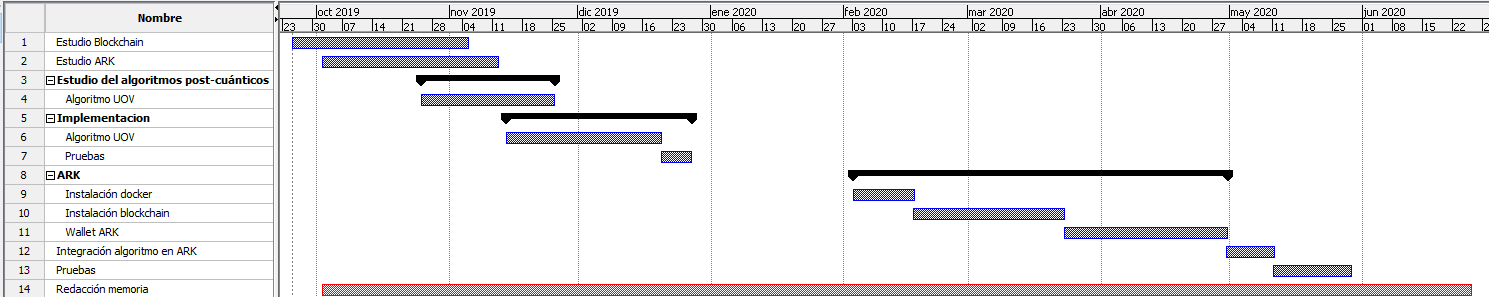
\includegraphics[width=14cm,height=5.5cm]{figuras/Gantt_ini.png}
	\caption{Digrama de Gantt inicial}
	\label{fig:gantt-ini}
\end{figure}

Pero no todo ha sido como se había planificado, puesto que han surgido algunos imprevistos. A la hora de realizar la implementación del algoritmo UOV en \texttt{python} no existe una biblioteca para trabajar con matrices y cuerpos finitos al mismo tiempo, así ha aumentado el tiempo que se iba a dedicar al algoritmo. Además el trabajo con ARK ha sido más tedioso del esperado, retrasando los tiempos programados. El diagrama de Gantt real se ha divido en parte para que se visualice mejor, la imagen \ref{fig:gantt-real-1} muestra las fases de estudio e implementación, la imagen \ref{fig:gantt-real-2} incluye el tiempo dedicado al trabajo con ARK hasta julio y la imagen \ref{fig:gantt-real-3} desde julio hasta noviembre, además del periodo de pruebas.\\


\begin{figure}[h]
	\centering
	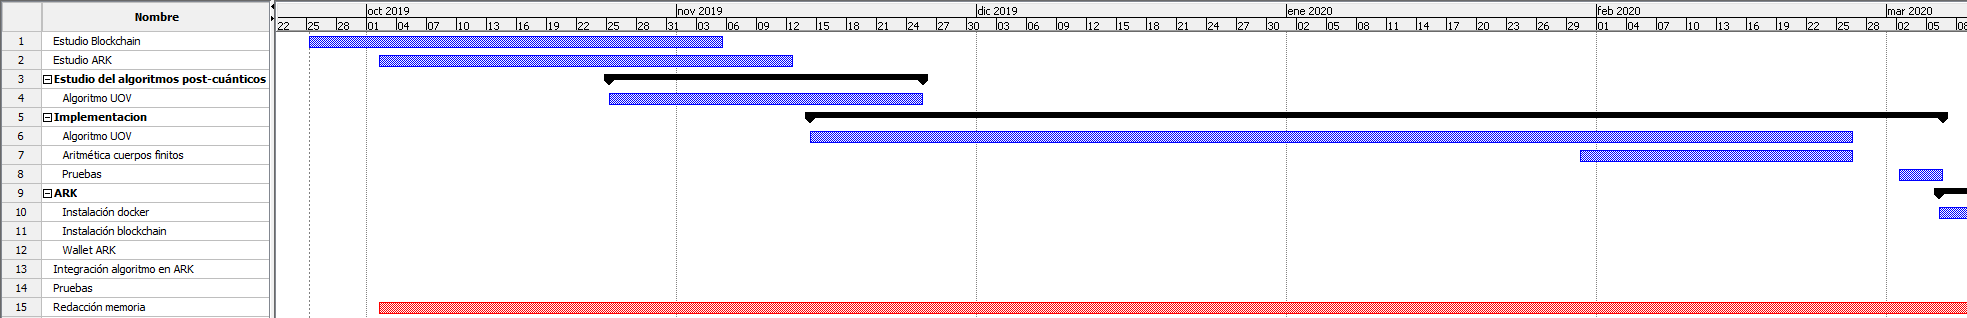
\includegraphics[width=15cm,height=6cm]{figuras/Gantt_1.png}
	\caption{Diagrama de Gantt real. Parte I}
	\label{fig:gantt-real-1}
\end{figure}

\begin{figure}[h]
	\centering
	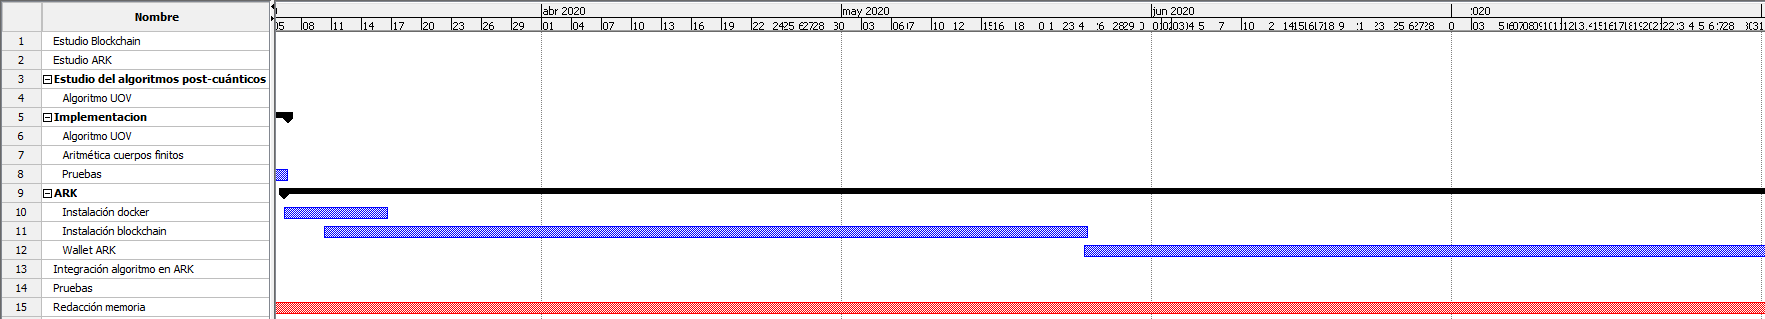
\includegraphics[width=15cm,height=6cm]{figuras/Gantt_2.png}
	\caption{Diagrama de Gantt real. Parte II}
	\label{fig:gantt-real-2}
\end{figure}

\begin{figure}[h]
	\centering
	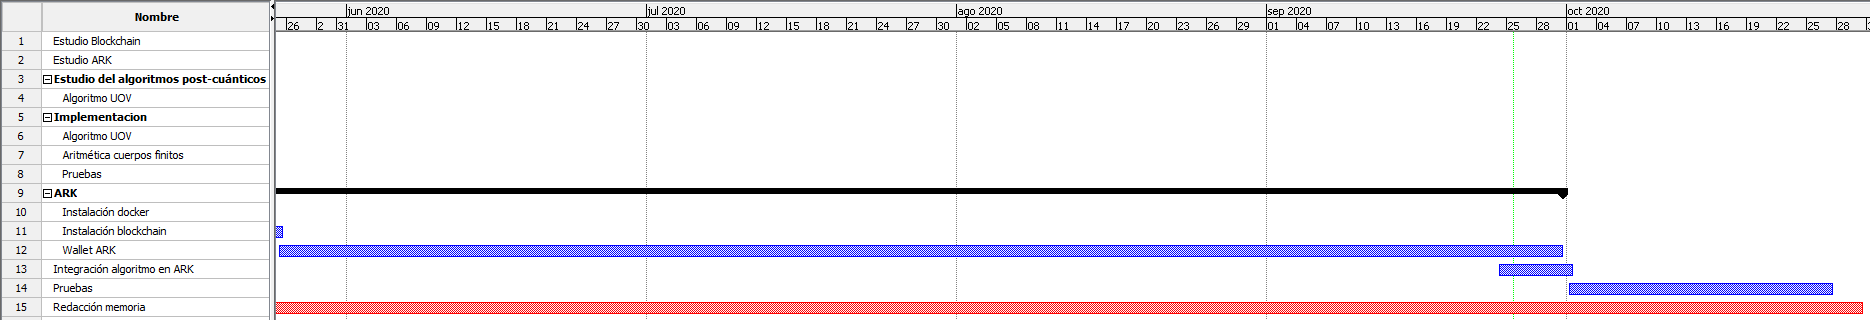
\includegraphics[width=15cm,height=6cm]{figuras/Gantt_3.png}
	\caption{Diagrama de Gantt real. Parte III}
	\label{fig:gantt-real-3}
\end{figure}

\section{Costes}
	\chapter{Análisis del problema}

Este tercer capítulo incluye una descripción de las funcionalidades que se pretenden alcanzar, así como de los problemas que han podido surgir para no llegar al diseño propuesto inicialmente. También se puede encontrar una especificación tanto los requisitos funcionales como los no funcionales.

\section{Especificación de requisitos}

Con la realización de este proyecto se persiguen principalmente dos funcionalidades, la implementación del algoritmo UOV y la integración del mismo en la \textit{blockchain}.

Para la implementación del algoritmo ha sido necesario implementar la aritmética de $\GF(128)$ puesto que no se ha encontrado ninguna librería de \texttt{python} que trabaje conjuntamente las matrices con cuerpos finitos. Se ha optado por el lenguaje de programación \texttt{python} para el algoritmo porque inicialmente se pensaba trabajar con la \textit{blockchain} implementada en \texttt{python} y no tener problemas a la hora de llamar a las funciones del algoritmo. Sin embargo tras un proceso de investigación se vió mejor opción utilizar la \textit{blockchain} en \texttt{typescript} para hacer uso de la parte gráfica como es la aplicación wallet y el \textit{explorer}. De esta forma se ha visto afectado el diseño inicial puesto que han sido necesarios dos ficheros más de transición entre los ficheros de \texttt{typescript} y \texttt{python}, se entrará en detalle en el capítulo \ref{sec:diseno}.

\subsection{Requisitos funcionales}

La especificación de los requisitos funcionales se ha dividido en varios apartados según cada parte del proyecto. Se distinguen, el programa en \texttt{python} con la implementación del algoritmo UOV, tabla \ref{tab:RF-pro}, el docker que contiene la interacción con la base de datos y la \textit{blockchain}, tabla \ref{tab:RF-docker}, la aplicación wallet desde donde se realizarán las transacciones, tabla \ref{tab:RF-wallet} y por último, el \textit{explorer} para visualizar las transacciones realizadas y los bloques generados, tabla \ref{tab:RF-exp}.

\begin{table}[H]
	\begin{center}
	\centering
	\resizebox{\linewidth}{!}{
	\begin{tabular}{p{0.14\linewidth} p{0.75\linewidth}}
		\textbf{Requisito} & \textbf{Descripción} \\
		\toprule
		RF 1.1 & El programa deberá tener la implementación de la aritmética de $\GF(128)$\\[0.5ex]
		RF 1.2 & El programa deberá de generar la clave pública y privada de cada usuario\\[0.5ex]
		RF 1.3 & El programa deberá de firmar correctamente cada \textit{hash}, ya sea de un bloque o una transacción\\[0.5ex]
		RF 1.4 & El programa deberá de realizar correctamente la verificación de un \textit{hash} con una firma\\[0.5ex]
		\bottomrule
	\end{tabular}}
	\end{center}
	\caption{Requisitos funcionales del programa}
	\label{tab:RF-pro}
\end{table}


\begin{table}[H]
	\begin{center}
	\centering
	\resizebox{\linewidth}{!}{
	\begin{tabular}{p{0.14\linewidth} p{0.75\linewidth}}
		\textbf{Requisito} & \textbf{Descripción} \\
		\toprule
		RF 2.1 & La base de datos local del docker deberá almacenar la claves del usuario\\[0.5ex]
		RF 2.2 & La base de datos local del docker deberá almacenar la información del usuario\\[0.5ex]
		RF 2.3 & La base de datos local del docker deberá almacenar los monederos así como el saldo de cada usuario\\[0.5ex]
		RF 2.4 & El docker deberá de almacenar la \textit{blockchain}\\[0.5ex]
		RF 2.5 & El docker deberá mantener activa la ejecución de la \textit{blockchain}\\[0.5ex]
		RF 2.6 & El docker deberá mantener activa la ejecución del \textit{explorer}\\[0.5ex]
		RF 2.7 & El docker deberá mantener abiertos los puertos del \textit{explorer} y API\\[0.5ex]
		RF 2.8 & El docker tendrá integrado la \textit{blockchain} con el nuevo código de firma\\[0.5ex]
		RF 2.9 & El docker tendrá integrado la \textit{blockchain} con el nuevo código de verificación\\[0.5ex]
		\bottomrule
	\end{tabular}}
	\end{center}
	\caption{Requisitos funcionales del docker}
	\label{tab:RF-docker}
\end{table}

\begin{table}[H]
	\begin{center}
	\centering
	\resizebox{\linewidth}{!}{
	\begin{tabular}{p{0.14\linewidth} p{0.75\linewidth}}
		\textbf{Requisito} & \textbf{Descripción} \\
		\toprule
		RF 3.1 & La aplicación deberá dar la opción al usuario de crear un perfil\\[0.5ex]
		RF 3.2 & La aplicación deberá dar la opción al usuario de conectarse a la red \textit{testnet}\\[0.5ex]
		RF 3.3 & La aplicación deberá dar la opción al usuario de importar el monedero genesis\\[0.5ex]
		RF 3.4 & La aplicación deberá dar la opción al usuario de crear monederos\\[0.5ex]
		RF 3.5 & La aplicación deberá dar la opción al usuario realizar transacciones entre diferentes monederos\\[0.5ex]
		RF 3.6 & La aplicación deberá dar la opción al usuario de firmar mensajes\\[0.5ex]
		RF 3.7 & La aplicación deberá dar la opción al usuario de validar mensajes\\[0.5ex]
		
		\bottomrule
	\end{tabular}}
	\end{center}
	\caption{Requisitos funcionales de la aplicación Wallet}
	\label{tab:RF-wallet}
\end{table}

\begin{table}[H]
	\begin{center}
	\centering
	\resizebox{\linewidth}{!}{
	\begin{tabular}{p{0.14\linewidth} p{0.75\linewidth}}
		\textbf{Requisito} & \textbf{Descripción} \\
		\toprule
		RF 4.1 & En el \textit{explorer} se podrá realizar búsqueda por bloques\\[0.5ex]
		RF 4.2 & En el \textit{explorer} se podrá realizar búsqueda por transacciones\\[0.5ex]
		RF 4.3 & El \textit{explorer} deberá mostrar la firma de cada bloque \\[0.5ex]
		RF 4.4 & El \textit{explorer} deberá mostrar el ID de cada bloque\\[0.5ex]
		RF 4.5 & El \textit{explorer} deberá mostrar la firma de cada transacción \\[0.5ex]
		RF 4.6 & El \textit{explorer} deberá mostrar el usuario que ha realizado la transacción además del receptor\\[0.5ex]
		RF 4.7 & Los datos que muestre el \textit{explorer} deberán de ser a tiempo real\\[0.5ex]
		
		\bottomrule
	\end{tabular}}
	\end{center}
	\caption{Requisitos funcionales del \textit{Explorer}}
	\label{tab:RF-exp}
\end{table}


\subsection{Requisitos no funcionales}

En los requisitos no funcionales podemos encontrar dos bloques, los referentes al sistema como los tiempos de ejecución o a la seguridad, tabla \ref{tab:RNF-sis}, y los personales, que logros esperaba conseguir tras la finalización del proyecto, tabla \ref{tab:RNF-per}

\begin{table}[H]
	\begin{center}
	\centering
	\resizebox{\linewidth}{!}{
	\begin{tabular}{p{0.14\linewidth} p{0.75\linewidth}}
		\textbf{Requisito} & \textbf{Descripción} \\
		\toprule
		RNF 1.1 & El programa no deberá de tardar más de medio minuto en generar las claves públicas y privadas \\[0.5ex]
		RNF 1.2 & El programa deberá de tardar unos segundos en firmar un mensaje\\[0.5ex]
		RNF 1.3 & El programa deberá de tardar unos segundos en verificar la firma de un $hash$\\[0.5ex]
		RNF 1.4 & En cualquier momento se podrá realizar la verificación de una firma\\[0.5ex]
		RNF 1.5 & El programa deberá de ser correctamente integrado en el sistema \textit{blockchain}\\[0.5ex]
		RNF 1.6 & El programa deberá de ser compatible con cualquier sistema compatible con \texttt{python}\\[0.5ex]
		RNF 1.7 & La aplicación deberá de realizar transacciones de forma segura\\[0.5ex]
		RNF 1.8 & El proyecto deberá de contar con un manual de usuario claro y conciso\\[0.5ex]
		\bottomrule
	\end{tabular}}
	\end{center}
	\caption{Requisitos no funcionales del sistema}
	\label{tab:RNF-sis}
\end{table}

\begin{table}[H]
	\begin{center}
	\centering
	\resizebox{\linewidth}{!}{
	\begin{tabular}{p{0.14\linewidth} p{0.75\linewidth}}
		\textbf{Requisito} & \textbf{Descripción} \\
		\toprule
		RNF 2.1 & Aprender a gestionar los tiempos de un proyecto\\[0.5ex]
		RNF 2.2 & Aprender a solucionar de la manera más eficiente los problemas que surjan\\[0.5ex]
		RNF 2.3 & Aprender otros lenguajes de programación como \texttt{python}\\[0.5ex]
		RNF 2.4 & Entender como funcionan la tecnología \textit{blockchain}\\[0.5ex]
		RNF 2.5 & Entender el algoritmo El programa deberá de ser correctamente integrado en el sistema \textit{blockchain}\\[0.5ex]
		RNF 2.6 & El programa deberá de ser compatible con cualquier sistema compatible con \texttt{python}\\[0.5ex]
		RNF 2.7 & La aplicación deberá de realizar transacciones de forma segura\\[0.5ex]
		RNF 2.8 & El proyecto deberá de contar con un manual de usuario claro y conciso\\[0.5ex]
		\bottomrule
	\end{tabular}}
	\end{center}
	\caption{Requisitos no funcionales personales}
	\label{tab:RNF-per}
\end{table}

\section{Análisis}

El objetivo de este apartado es mostrar en diferentes subapartados los diferentes subproblemas que han aparecido al realizar el proyecto, describiendo las alternativas que se han considerado, y justificando las decisiones que se han adoptado. A veces, especialmente cuando los conceptos utilizados en este apartado son extensos, es necesario clarificarlos previamente en el Capítulo de \textit{Introducción} (sección \textit{Contenidos teóricos para la comprensión del proyecto}).   
	\chapter{Diseño}

%Es uno de los capítulos más importantes. Debe explicar claramente la solución propuesta justificando la aproximación adoptada. Este capítulo, según el caso, es aconsejable que defina claramente la arquitectura del sistema propuesto, identificando los roles o partes o actores del sistema. Pueden emplearse metodologías basadas en diagramas de clases, paquetes, diagramas secuenciales, diagramas de relación, etc.

%Si se ha diseñado una interfaz gráfica debe también describirse su estructura, dónde se mostrará la información, etc.

\section{Algoritmo criptográfico}

La estructura del algoritmo viene dada por un fichero escrito en python donde se encuentran las funciones que se explicarán en detalle en el capítulo \ref{sec:implementacion}.

El fichero \texttt{luov.py} incorpora main con un ejemplo de uso del algoritmo independientemente de la \textit{blockchain}.

\section{Ecosistema ARK}

El ecosistema ark se ha instalado en un docker \texttt{ubuntu:xenial}. Nos encontramos con las carpetas deployer, core-bridgechain y core-explorer.

La carpeta deployer contiene la instalación de la \textit{blockchain} y del \textit{explorer}. Para instalar la blockchain y el explorer se hara mediante la ejecucion del archivo bridgechain.sh con los convenientes parámetros.

	\chapter{Implementación}
\label{sec:implementacion}
%Aquí se deben proporcionar los detalles de cómo se ha llevado a la práctica el diseño propuesto en el capítulo anterior. Deben identificarse claramente herramientas, tecnologías, equipamientos, etc. utilizados o necesarios para el buen funcionamiento de la solución. Se pueden describir los fragmentos de código más importantes, con el fin de clarificar la funcionalidad que proporcionan. En general este capítulo debe facilitar la reutilización de nuestra solución, por lo que debe estar bien documentada. Puede incluir un manual de uso.

Aquí se proporcionan los detalles de las funciones implementadas para la ejecución algoritmo UOV, además de la implementación de la aritmética en el cuerpo de 128 elementos.\\

\section{Funciones del cuerpo de 128 elementos}
Las funciones referentes a esta sección son la suma, el producto y conversiones de elementos del cuerpo de $2$ elementos a elementos del cuerpo de $128$ elementos.\\

Los elementos del cuerpo se representarán con vectores de siete componentes para poder facilitar la implementación de la suma y del producto. Esto se refleja en las dos tablas denominadas \texttt{exp} y \texttt{log}, que tienen la estructura que se muestra en los códigos \ref{cod:exp} y \ref{cod:log}, respectivamente. Para la implementación se han usado las variables diccionario de \texttt{python}, puesto que tienen fácil acceso a todas las componentes.

\vspace{0.25cm}

\begin{lstlisting}[language=Python,caption=Tabla para calcular la potencia en el cuerpo, label=cod:exp]
exp = {
   0 : [0, 0, 0, 0, 0, 0, 1],
   1 : [0, 0, 0, 0, 0, 1, 0],
   125 : [1, 1, 0, 0, 0, 0, 1],
   126 : [1, 0, 0, 0, 0, 0, 1]
}

\end{lstlisting}

\begin{lstlisting}[language=Python,caption=Tabla para calcular el logaritmo en el cuerpo, label=cod:log]
log = {
   tuple( [0, 0, 0, 0, 0, 0, 1] ) : ' 0 ',
   tuple( [0, 0, 0, 0, 0, 1, 0] ) : ' 1 ',
   tuple( [1, 1, 0, 0, 0, 0, 1] ) : ' 125 ',
   tuple( [1, 0, 0, 0, 0, 0, 1] ) : ' 126 ',
}
\end{lstlisting}

La suma de dos elementos del cuerpo se ha implementando la puerta $xor$, esto es si las $iésimas$-componentes son iguales entonces la suma vale $0$, en caso contrario vale $1$, código \ref{cod:suma-cuerpo}.

\begin{table}[h]
	\begin{center}
	\centering
	\resizebox{\linewidth}{!}{
	\begin{tabular}{p{0.14\linewidth} p {0.1\linewidth}p{0.1\linewidth}p{0.65\linewidth}}
		\textbf{Tipo} & \textbf{Nombre} & \textbf{Variable} & \textbf{Descripción} \\
		\toprule
		int vector & n1 & Input & Elemento para sumar de $\GF(128)$\\[0.5ex]
		int vector & n2 & Input & Elemento para sumar de $\GF(128)$\\[0.5ex]
		int vector & suma & Output & Elemento  del cuerpo que almacena la suma de n1 y n2\\[0.5ex]
		\bottomrule
	\end{tabular}}
	\end{center}
	\caption{Parámetros de la función \texttt{suma}}
\end{table}

\vspace{0.25cm}
\begin{lstlisting}[language=Python,caption=Suma de dos elementos del cuerpo, label=cod:suma-cuerpo]
def suma(n1=[], n2=[]):

   suma = []
   for i in range(len(n1)):
      if n1[i] == n2[i]:
         suma += [0]
      else:
         suma += [1]
   return suma
\end{lstlisting}

Para el producto de dos elementos del cuerpo se ha diferenciado el caso en el que uno de los vectores sea $0$ en dicho caso el producto vale $0$. Si ninguno de los vectores es $0$ entonces se hace uso de las tablas \ref{cod:exp} y \ref{cod:log}, para trabajar con enteros módulo $127$, código \ref{cod:producto-cuerpo}.

\begin{table}[h]
	\begin{center}
	\centering
	\resizebox{\linewidth}{!}{
	\begin{tabular}{p{0.14\linewidth} p {0.1\linewidth}p{0.1\linewidth}p{0.65\linewidth}}
		\textbf{Tipo} & \textbf{Nombre} & \textbf{Variable} & \textbf{Descripción} \\
		\toprule
		int vector & n1 & Input & Elemento para multiplicar de $\GF(128)$\\[0.5ex]
		int vector & n2 & Input & Elemento para multiplicar de $\GF(128)$\\[0.5ex]
		int & suma & Inner & Almacena la suma de los logaritmos de n1 y n2 módulo 127\\[1.5ex]
		int vector & product & Output & Elemento del cuerpo que almacena el producto de n1 y n2\\[0.5ex]
		\bottomrule
	\end{tabular}}
	\end{center}
	\caption{Parámetros de la función \texttt{product}}
\end{table}

\vspace{0.25cm}
\begin{lstlisting}[language=Python,caption=Producto de dos elementos del cuerpo, label=cod:producto-cuerpo]
def product(n1=[], n2=[]):

   product = []
   if (n1 == [0,0,0,0,0,0,0]) or (n2 == [0,0,0,0,0,0,0]):
      product = [0,0,0,0,0,0,0]
   else:
      suma = (int(log.get(tuple(n1))) + int(log.get(tuple(n2))))%127
      product = exp.get(suma)
   return product
\end{lstlisting}


Las siguientes funciones son necesarias para la resolución del sistema de ecuaciones.


Calcula el vector correspondiente vector en el cuerpo de un entero, código \ref{cod:entero-cuerpo}.


\begin{table}[h]
	\begin{center}
	\centering
	\resizebox{\linewidth}{!}{
	\begin{tabular}{p{0.14\linewidth} p {0.1\linewidth}p{0.1\linewidth}p{0.65\linewidth}}
		\textbf{Tipo} & \textbf{Nombre} & \textbf{Variable} & \textbf{Descripción} \\
		\toprule
		int & n1 & Input & Entero del que se desea calcular su vector en el cuerpo\\[1.5ex]
		int vector &  & Output & Elemento de $\GF(128)$\\[0.5ex]
		\bottomrule
	\end{tabular}}
	\end{center}
	\caption{Parámetros de la función \texttt{F128}}
\end{table}
\vspace{0.25cm}

\begin{lstlisting}[language=Python,caption=Convierte un entero en un elemento del cuerpo, label=cod:entero-cuerpo]
def F128(n1):

   if n1 == 127:
      return [0,0,0,0,0,0,0]
   else:
      return exp.get(n1)
\end{lstlisting}


Al estar en un cuerpo todo elementos tiene inverso y tiene sentido hacer la función \texttt{inverso} de un elemento del cuerpo, la implementación que se ha hecho ha sido hacer la multiplicación por los restantes elementos y comprobando que de como resultado el elemento unidad, en este caso $[0,0,0,0,0,0,1]$, código \ref{cod:inverso-cuerpo}.

\begin{table}[h]
	\begin{center}
	\centering
	\resizebox{\linewidth}{!}{
	\begin{tabular}{p{0.14\linewidth} p {0.1\linewidth}p{0.1\linewidth}p{0.65\linewidth}}
		\textbf{Tipo} & \textbf{Nombre} & \textbf{Variable} & \textbf{Descripción} \\
		\toprule
		int vector & n & Input & Elemento para calcular su inverso en $\GF(128)$\\[1.5ex]
		int vector &  & Output & Inverso de n\\[0.5ex]
		\bottomrule
	\end{tabular}}
	\end{center}
	\caption{Parámetros de la función \texttt{inverse}}
\end{table}

\vspace{0.25cm}
\begin{lstlisting}[language=Python,caption=Inverso de un elemento del cuerpo, label=cod:inverso-cuerpo]
def inverse(n=[]):

   i = 0
   while product(n, F128(i)) != [0,0,0,0,0,0,1]:
      i += 1
   return F128(i)
\end{lstlisting}

La función \texttt{mayor} compara si el elemento $n1$ es mayor que el elemento $n2$, para ello se convierten los vectores a enteros con la tabla \texttt{log} y se compara que entero es mayor, código \ref{cod:mayor-que-cuerpo}.

\begin{table}[h]
	\begin{center}
	\centering
	\resizebox{\linewidth}{!}{
	\begin{tabular}{p{0.14\linewidth} p {0.1\linewidth}p{0.1\linewidth}p{0.65\linewidth}}
		\textbf{Tipo} & \textbf{Nombre} & \textbf{Variable} & \textbf{Descripción} \\
		\toprule
		int vector & n1 & Input & Elemento a comparar con n2 en $\GF(128)$\\[0.5ex]
		int vector & n2 & Input & Elemento a comparar con n1 en $\GF(128)$\\[1.5ex]
		int & log1 & Inner & Almacena el logaritmo de n1\\[0.5ex]
		int & log2 & Inner & Almacena el logaritmo de n2\\[1.5ex]
		boolean &  & Output & \texttt{True} si n1 es mayor\\
		& & & \texttt{False} en otro caso\\[0.5ex]
		\bottomrule
	\end{tabular}}
	\end{center}
	\caption{Parámetros de la función \texttt{mayor}}
\end{table}

\vspace{0.25cm}

\begin{lstlisting}[language=Python,caption=Compara dos elementos del cuerpo, label=cod:mayor-que-cuerpo]
def mayor (n1=[],n2=[]):

   if n1 == [0,0,0,0,0,0,0]:
      return False
   else:
      log1, log2 = log.get(tuple(n1)), log.get(tuple(n2))
      return int(log1) > int(log2)
\end{lstlisting}
 


Convierte una matriz $n1$ del cuerpo $\mathds{F}_2$ en un vector $n$ de $\GF(128)$. Como los elementos de la matriz son solo 0 y 1 la conversión se reduce a, si en la matriz hay un 0 añade al vector $n$ el vector $[0,0,0,0,0,0,0]$ y en otro caso $[0,0,0,0,0,0,1]$, código \ref{cod:matrizF2-cuerpo}.

\begin{table}[h]
	\begin{center}
	\centering
	\resizebox{\linewidth}{!}{
	\begin{tabular}{p{0.14\linewidth} p {0.1\linewidth}p{0.1\linewidth}p{0.65\linewidth}}
		\textbf{Tipo} & \textbf{Nombre} & \textbf{Variable} & \textbf{Descripción} \\
		\toprule
		int vector & n1 & Input & Matriz con elementos en $\mathds{F}_2$\\[1.5ex]
		int & row & Inner & Almacena las filas generadas de la matriz n\\[1.5ex]
		int vector & n & Output & Matriz en $\GF(128)$\\[0.5ex]
		\bottomrule
	\end{tabular}}
	\end{center}
	\caption{Parámetros de la función \texttt{matrix\_F2to128}}
\end{table}

\vspace{0.25cm}
\begin{lstlisting}[language=Python,caption=Matriz de $\mathds{F}_2$ a un elemento del cuerpo 128 elementos, label=cod:matrizF2-cuerpo]
def matrix_F2to128(n1=[]):

   n =[]
   for i in range(len(n1)):
      row =[]
      for j in range(len(n1[0])):
         if n1[i][j] == 0:
            row += [[0,0,0,0,0,0,0]]
         else:
            row += [[0,0,0,0,0,0,1]]
      n += [row]
   return n
\end{lstlisting}


Convierte un vector de matrices $n1$ del cuerpo $\mathds{F}_2$ en una matriz $matrix$ del cuerpo de 128 elementos. Como en la función anterior los elementos de la matriz son solo 0 y 1, se aplica el mismo cambio, código \ref{cod:matriz3dF2-cuerpo}.

\begin{table}[h]
	\begin{center}
	\centering
	\resizebox{\linewidth}{!}{
	\begin{tabular}{p{0.14\linewidth} p {0.1\linewidth}p{0.1\linewidth}p{0.65\linewidth}}
		\textbf{Tipo} & \textbf{Nombre} & \textbf{Variable} & \textbf{Descripción} \\
		\toprule
		int vector & n1 & Input & Vector de matriz con elementos en $\mathds{F}_2$\\[1.5ex]
		int & n & Inner & Almacena las matrices del vector matrix\\[0.5ex]
		int & row & Inner & Almacena las filas generadas de la matriz n\\[1.5ex]
		int vector & matrix & Output & Vector de matrices con elementos en $\GF(128)$\\[0.5ex]
		\bottomrule
	\end{tabular}}
	\end{center}
	\caption{Parámetros de la función \texttt{matrix3d\_F2to128}}
\end{table}

\vspace{0.25cm}

\begin{lstlisting}[language=Python,caption=Vector de matrices de $\mathds{F}_2$ a una matriz de $\GF(128)$, label=cod:matriz3dF2-cuerpo]
def matrix3d_F2to128(n1=[]):

   matrix =[]
   for i in range(len(n1)):
      n = []
      for j in range(len(n1[0])):
         row = []
         for k in range(len(n1[0][0])):
            if n1[i][j][k] == 0:
               row += [[0,0,0,0,0,0,0]]
               
            else:
               row += [[0,0,0,0,0,0,1]]
         n += [row]
      matrix += [n]
   return matrix
\end{lstlisting}

\section{Funciones con matrices}

En esta sección de explicarán funciones como la suma de matrices, cálculo de la matriz transpuesta, matriz identidad y el producto de matrices tanto en $\mathds{F}_2$ como en $\GF(128)$. Además incluye la función que resuelve el sistema de ecuaciones con el método de Gauss-Jordan.\\


Suma de dos matrices $m1$ y $m2$ del cuerpo de 128 elementos, código \ref{cod:suma-matrix}.

\begin{table}[h]
	\begin{center}
	\centering
	\resizebox{\linewidth}{!}{
	\begin{tabular}{p{0.14\linewidth} p {0.1\linewidth}p{0.1\linewidth}p{0.65\linewidth}}
		\textbf{Tipo} & \textbf{Nombre} & \textbf{Variable} & \textbf{Descripción} \\
		\toprule
		int vector & m1 & Input & Matriz a sumar en $\GF(128)$\\[0.5ex]
		int vector & m2 & Input & Matriz a sumar en $\GF(128)$\\[1.5ex]
		int & row & Inner & Almacena las filas de n\\[1.5ex]
		int vector & m\_suma & Output & Suma de las matrices m1 y m2 en $\GF(128)$\\[0.5ex]
		\bottomrule
	\end{tabular}}
	\end{center}
	\caption{Parámetros de la función \texttt{matrix\_sum}}
\end{table}

\vspace{0.25cm}

\begin{lstlisting}[language=Python,caption=Suma de dos matrices con elementos en el cuerpo, label=cod:suma-matrix]
def matrix_sum (m1, m2):

   m_suma = []

   if (len(m1) == len(m2)) and (len(m1[0]) == len(m2[0])):
      for i in range(len(m1)):
         row = []
         for j in range(len(m1[0])):
            row += [suma (m1[i][j], m2[i][j])]
         m_suma += [row]
   return m_suma
\end{lstlisting}


Producto de dos matrices con elementos en el cuerpo de 128 elementos, código \ref{cod:prod-matrix}.

\begin{table}[h]
	\begin{center}
	\centering
	\resizebox{\linewidth}{!}{
	\begin{tabular}{p{0.14\linewidth} p {0.1\linewidth}p{0.1\linewidth}p{0.65\linewidth}}
		\textbf{Tipo} & \textbf{Nombre} & \textbf{Variable} & \textbf{Descripción} \\
		\toprule
		int vector & n1 & Input & Matriz a multiplicar en $\GF(128)$\\[0.5ex]
		int vector & n2 & Input & Matriz a multiplicar en $\GF(128)$\\[1.5ex]
		int & p\_suma & Inner & Almacena la suma de los productos de cada elemento de la fila de n1 y de la columna de n2\\[0.5ex]
		int & row & Inner & Almacena las filas de prod\\[0.5ex]
		int vector & prod & Output & Producto de las matrices m1 y m2 en $\GF(128)$\\[0.5ex]
		\bottomrule
	\end{tabular}}
	\end{center}
	\caption{Parámetros de la función \texttt{matrix\_product}}
\end{table}

\vspace{0.25cm}

\begin{lstlisting}[language=Python,caption=Producto de matrices con elementos del cuerpo, label=cod:prod-matrix]
def matrix_product (n1=[], n2=[]):

   prod=[]
   if len(n1[0]) == len(n2):
      for i1 in range(len(n1)):
         row = []
         for j in range(len(n2[0])):
            p_suma = [0,0,0,0,0,0,0]
            for i2 in range(len(n2)):
               p_suma = suma (product(n1[i1][i2], n2[i2][j]), p_suma)
            row += [p_suma]
         prod += [row]
   return prod
\end{lstlisting}

Producto de dos matrices con elementos en el cuerpo $\mathds{F}_2$, como los elementos de la matriz son $0$ y $1$ la suma acomulada se hace con la operación lógica \texttt{xor},  código \ref{cod:prodF2-matrix}.

\begin{table}[h]
	\begin{center}
	\centering
	\resizebox{\linewidth}{!}{
	\begin{tabular}{p{0.14\linewidth} p {0.1\linewidth}p{0.1\linewidth}p{0.65\linewidth}}
		\textbf{Tipo} & \textbf{Nombre} & \textbf{Variable} & \textbf{Descripción} \\
		\toprule
		int vector & n1 & Input & Matriz a multiplicar en $\mathds{F}_2$\\[0.5ex]
		int vector & n2 & Input & Matriz a multiplicar en $\mathds{F}_2$\\[1.5ex]
		int & p\_suma & Inner & Almacena la suma de los productos de cada elemento de la fila de n1 y de la columna de n2\\[0.5ex]
		int & row & Inner & Almacena las filas de prod\\[1.5ex]
		int vector & prod & Output & Producto de las matrices m1 y m2 en $\mathds{F}_2$\\[0.5ex]
		\bottomrule
	\end{tabular}}
	\end{center}
	\caption{Parámetros de la función \texttt{matrix\_product\_F2}}
\end{table}

\vspace{0.25cm}

\begin{lstlisting}[language=Python,caption=Producto de matrices con elementos en $\mathds{F}_2$, label=cod:prodF2-matrix]
def matrix_product_F2 (n1=[], n2=[]):

   prod=[]
   if len(n1[0]) == len(n2):
      for i1 in range(len(n1)):
         row = []
         for j in range(len(n2[0])):
            p_suma = 0
            for i2 in range(len(n2)):
               p_suma = (n1[i1][i2] * n2[i2][j]) ^ p_suma
            row += [p_suma]
         prod += [row]
   return prod
\end{lstlisting}

Calcula la matriz transpuesta de la matriz dada como parámetro, código \ref{cod:trans-matrix}.

\begin{table}[h]
	\begin{center}
	\centering
	\resizebox{\linewidth}{!}{
	\begin{tabular}{p{0.14\linewidth} p {0.1\linewidth}p{0.1\linewidth}p{0.65\linewidth}}
		\textbf{Tipo} & \textbf{Nombre} & \textbf{Variable} & \textbf{Descripción} \\
		\toprule
		int vector & m & Input & Matriz para calcular su transpuesta\\[1.5ex]
		int & row & Inner & Almacena las filas de trans\\[1.5ex]
		int vector & trans & Output & Matriz transpuesta\\[0.5ex]
		\bottomrule
	\end{tabular}}
	\end{center}
	\caption{Parámetros de la función \texttt{matrix\_transpose}}
\end{table}

\vspace{0.25cm}

\begin{lstlisting}[language=Python,caption=Matriz transpuesta, label=cod:trans-matrix]
def matrix_transpose(m):

   trans = []
   for j in range(len(m[0])):
      row = []
      for i in range(len(m)):
         row += [m[i][j]]
      trans += [row]
   return trans
\end{lstlisting}


Calcula la matriz identidad con una determinada dimensión, $dim$, que se pasa como parámetro, código \ref{cod:identi-matrix}.

\begin{table}[h]
	\begin{center}
	\centering
	\resizebox{\linewidth}{!}{
	\begin{tabular}{p{0.14\linewidth} p {0.1\linewidth}p{0.1\linewidth}p{0.65\linewidth}}
		\textbf{Tipo} & \textbf{Nombre} & \textbf{Variable} & \textbf{Descripción} \\
		\toprule
		int & dim & Input & Dimensión de la que calcular la matriz identidad en $\GF(128)$\\[1.5ex]
		int & row & Inner & Almacena las filas de matrix\\[1.5ex]
		int vector & matrix & Output & Matriz identidad\\[0.5ex]
		\bottomrule
	\end{tabular}}
	\end{center}
	\caption{Parámetros de la función \texttt{matrix\_identity}}
\end{table}

\vspace{0.25cm}

\begin{lstlisting}[language=Python,caption=Matriz identidad del cuerpo, label=cod:identi-matrix]
def matrix_identity(dim):

   matrix = []

   for i in range(dim):
      row = []
      for j in range(dim):
         if i == j:
            row += [[0,0,0,0,0,0,1]]
         else:
            row += [[0,0,0,0,0,0,0]]
      matrix += [row]
   return matrix
\end{lstlisting}


La función \texttt{matrix\_rref} resuelve de un sistema de ecuaciones con el método de Gauss-Jordan, código \ref{cod:Gauss-matrix}. El sistema de ecuaciones es de la forma de la ecuación \ref{eq:Gauss}.

\begin{equation}\label{eq:Gauss}
A\cdot x=b
\end{equation}

\begin{table}[h]
	\begin{center}
	\centering
	\resizebox{\linewidth}{!}{
	\begin{tabular}{p{0.14\linewidth} p {0.1\linewidth}p{0.1\linewidth}p{0.65\linewidth}}
		\textbf{Tipo} & \textbf{Nombre} & \textbf{Variable} & \textbf{Descripción} \\
		\toprule
		int vector & A & Input & Matriz de la ecuación\\[0.5ex]
		int vector & b & Input & Vector de la ecuación\\[1.5ex]
		int vector & M & Inner & Matriz aumentada, combinación de A y b\\[1.5ex]
		int vector & x & Output & Solución del sistema\\[0.5ex]
		\bottomrule
	\end{tabular}}
	\end{center}
	\caption{Parámetros de la función \texttt{matrix\_rref}}
\end{table}

\vspace{0.25cm}

\begin{lstlisting}[language=Python,caption=Método de Gauss-Jordan, label=cod:Gauss-matrix]
def matrix_rref(A, b):

   r = 0
   row = []
   n = len(A)

   #Matriz aumentada, añadir b como una columna
   M = A
   for i in range(len(M)):
      M[i] += b[i]

   for k in range(n):
      #Intercambio de filas para que quede arriba la de menor valor
      for i in range(k, n):
         if mayor(M[i][k], M[k][k]):
            row = M[k]
            M[k] = M[i]
            M[i] = row

      #Hacer ceros
      for j in range(k+1, n):
         q = product(M[j][k], inverse(M[k][k]))
         for m in range(k, n+1):
            M[j][m] = suma(M[j][m], product(q, M[k][m]))

   #Calcular la solución x de abajo arriba
   x = [[[0,0,0,0,0,0,0]] for i in range(n)]

   x[n-1] = [product(M[n-1][n], inverse(M[n-1][n-1]))]
   for i in range(n-1, -1, -1):
      z = [0,0,0,0,0,0,0]
      for j in range(i+1, n):
         z = suma(z, product(M[i][j], x[j][0]))
      x[i] = [product(suma(M[i][n], z), inverse(M[i][i]))]

   return x
\end{lstlisting}

\section{Funciones algoritmo UOV}

La función \texttt{clavePrivada} genera la clave privada de un usuario, para ello genera una matriz triangular superior, $\alpha$, en $\mathds{F}_2$ con valores aleatorios, y un vector, $\beta$, en $\mathds{F}_2$. Los parámetros $m$ y $v$ son el número de variables de aceite y vinagre, respectivamente, código \ref{cod:priv-UOV}.

\vspace{-0.23cm}
\begin{table}[h]
	\begin{center}
	\centering
	\resizebox{\linewidth}{!}{
	\begin{tabular}{p{0.14\linewidth} p {0.1\linewidth}p{0.1\linewidth}p{0.65\linewidth}}
		\textbf{Tipo} & \textbf{Nombre} & \textbf{Variable} & \textbf{Descripción} \\
		\toprule
		int vector & m & Input & Número de aceites\\[0.5ex]
		int vector & v & Input & Número de vinagres\\[1.5ex]
		int vector & alpha & Output & Vector de matrices triangulares superiores aleatorias en $\mathds{F}_2$, parte de la clave privada \\[0.5ex]
		int vector & beta & Output & Matriz aleatoria en $\mathds{F}_2$, parte de la clave privada\\[0.5ex]
		\bottomrule
	\end{tabular}}
	\end{center}
	\caption{Parámetros de la función \texttt{clavePrivada}}
\end{table}


\begin{lstlisting}[language=Python,caption=Generación clave privada, label=cod:priv-UOV]
def clavePrivada (m, v):

   alpha, beta = [], []
   n = m+v

   for k in range(m):
      #alpha matriz triangular superior
      aux = []
      for i in range (v):
         row = []
         for j in range (n):
            if i > j:
               row += [0]
            else:
               row += [randint(0,1)]
         aux += [row]
      alpha += [aux]

      #beta
      row = []
      for i in range(n):
         if randint(0,1) == 0:
            row += [randint(0,1)]

      beta += [row]
   return alpha, beta
\end{lstlisting}

La función \texttt{generacionT} genera la matriz de distorsión $T$ a partir de los valores $m$ y $v$, número de variables de aceite y vinagre, código \ref{cod:T}. La forma de la matriz de distorsión viene dada por la ecuación \ref{mat:T}.

\begin{table}[h]
	\begin{center}
	\centering
	\resizebox{\linewidth}{!}{
	\begin{tabular}{p{0.14\linewidth} p {0.1\linewidth}p{0.1\linewidth}p{0.65\linewidth}}
		\textbf{Tipo} & \textbf{Nombre} & \textbf{Variable} & \textbf{Descripción} \\
		\toprule
		int vector & m & Input & Número aceites\\[0.5ex]
		int vector & v & Input & Número vinagres\\[0.5ex]
		int matrix & T & Output & Matriz en $\mathds{F}_2$ de dimensión $n\mathrm{x}n$\\[0.5ex]
		\bottomrule
	\end{tabular}}
	\end{center}
	\caption{Parámetros de la función \texttt{generacionT}}
\end{table}

\vspace{0.25cm}

\begin{lstlisting}[language=Python,caption=Generación matriz $T$, label=cod:T]
def generacionT (v, m):
   T = []
   n = v + m
   for i in range(n):
      row = []
      if i < v:
         for k in range(n):
            if k < v: #Matriz indentidad dimension v
               if i == k:
                  row += [1]
               else:
                  row += [0]

            else: #Matriz aleatoria vxm
               if randint(0,2) == 1:
                  row += [1]
               else:
                  row += [0]

      else:
         for k in range(n):
            if k < v: #Matriz nula dimension v
               row += [0]

            else: #Matriz identidad dimension m
               if i == k:
                  row += [1]
               else:
                  row += [0]
      T += [row]
   return T
\end{lstlisting}

La función \texttt{clavePublica} genera la clave pública a partir de la clave privada, calculada con la función anterior, los valores $m$ y $v$ el número de variables de aceite y vinagre, además de una matriz de distorsión, código \ref{cod:pub-UOV}.

\begin{table}[h]
	\begin{center}
	\centering
	\resizebox{\linewidth}{!}{
	\begin{tabular}{p{0.14\linewidth} p {0.1\linewidth}p{0.1\linewidth}p{0.65\linewidth}}
		\textbf{Tipo} & \textbf{Nombre} & \textbf{Variable} & \textbf{Descripción} \\
		\toprule
		int vector & m & Input & Número aceites\\[0.5ex]
		int vector & v & Input & Número vinagres\\[0.5ex]
		int vector & alpha & Input & Vector de matrices triangulares superiores en $\mathds{F}_2$, parte de la clave privada \\[0.5ex]
		int vector & beta & Input & Matriz en $\mathds{F}_2$, parte de la clave privada\\[0.5ex]
		int vector & T & Input & Matriz de distorsión de la forma \ref{mat:T}\\[1.5ex]
		int vector & alpha\_pub & Output & Vector de matrices en $\mathds{F}_2$, parte de la clave pública\\[0.5ex]
		int vector & beta\_pub & Output & Matriz en $\mathds{F}_2$, parte de la clave pública\\[0.5ex]
		\bottomrule
	\end{tabular}}
	\end{center}
	\caption{Parámetros de la función \texttt{clavePublica}}
\end{table}

\vspace{0.25cm}

\begin{lstlisting}[language=Python,caption=Generación clave pública, label=cod:pub-UOV]
def clavePublica(m, v, alpha, beta, T):

   alpha_pub = []
   beta_pub = []
   T_trans = matrix_transpose(T[0:v])

   for k in range(len(alpha)):
      aux = matrix_product_F2(T_trans , alpha [k])
      alpha_pub += [matrix_product_F2(aux, T)]


      beta_pub += [matrix_product_F2([beta[k]], T)]

   return alpha_pub, beta_pub
\end{lstlisting}

La función \texttt{signature} calcula la firma del hash de un mensaje, $hashed$, con las claves privadas del usuario, $alpha\_F2$ y $beta\_F2$, el número de aceites y vinagres, $m$ y $v$, y con la matriz de transición, $T$. Se toman los vinagres aleatorios, se resuelve el sistema para calcular los aceites, y con la ecuación \ref{eq:firma} obtenemos la firma del mensaje, código \ref{cod:firma-UOV}.

\begin{table}[h]
	\begin{center}
	\centering
	\resizebox{\linewidth}{!}{
	\begin{tabular}{p{0.14\linewidth} p {0.1\linewidth}p{0.1\linewidth}p{0.65\linewidth}}
		\textbf{Tipo} & \textbf{Nombre} & \textbf{Variable} & \textbf{Descripción} \\
		\toprule
		int vector & hashed & Input & Vector \textit{hash}\\[0.5ex]
		int vector & alpha\_F2 & Input & Vector de matrices triangulares superiores en $\mathds{F}_2$, parte de la clave privada\\[0.5ex]
		int vector & beta\_F2 & Input & Matriz en $\mathds{F}_2$, parte de la clave privada \\[0.5ex]
		int  & m & Input & Número aceites\\[0.5ex]
		int  & v & Input & Número vinagres\\[0.5ex]
		int vector & T & Input & Matriz de distorsión de la forma \ref{mat:T}\\[1.5ex]
		int vector & alpha & Inner & Almecena los correspondientes valores de alpha\_F2 en $\GF(128)$\\[0.5ex]
		int vector & beta & Inner &  Almecena los correspondientes valores de beta\_F2 en $\GF(128)$\\[0.5ex]
		int vector & vinagre & Inner & Vector aleatorio de tamaño v, contiene los vinagres\\[0.5ex]
		int vector & coef & Inner & Almacena los coeficientes del sistema\\[0.5ex]
		int vector & term & Inner & Almacena los términos del sistema\\[0.5ex]
		int vector & oil & Inner & Almacena la solución del sistema, son los aceites del algoritmo\\[1.5ex]
		int vector & firma & Output & Contiene la firma de \textit{hashed}\\[0.5ex]
		\bottomrule
	\end{tabular}}
	\end{center}
	\caption{Parámetros de la función \texttt{signature}}
\end{table}

\vspace{0.25cm}

\begin{lstlisting}[language=Python,caption=Firma del mensaje, label=cod:firma-UOV]
def signature(hashed, alpha_F2, beta_F2, m, v, T):

   alpha = matrix3d_F2to128(alpha_F2)
   beta = matrix_F2to128(beta_F2)

   vinagre = []
   for k in range(v):
      aux = randint(0, 127)
      vinagre += [F128(aux)]
   coef = []
   term = []

   n= m + v
   for k in range(m):
      A = matrix_product([vinagre], alpha[k])
      coef += matrix_sum([A[0][v:n]], [beta[k][v:n]])
      v_suma = suma (matrix_product([A[0][0:v]], matrix_transpose([vinagre]))[0][0], matrix_product([beta[k][0:v]], matrix_transpose([vinagre]))[0][0])
      term += [suma(hashed[k], v_suma)]


   oil = matrix_rref(coef, matrix_transpose([term]))

   aux = []
   aux += vinagre + matrix_transpose(oil)[0]
   firma = matrix_product([aux], matrix_transpose(matrix_F2to128(T))) #T = T.inverse()
   return firma[0]
\end{lstlisting}

Por último la función \texttt{verify} comprueba si la firma, $firma$, de un mensaje, $m$, es correcta, para ello utiliza las claves públicas del usuario y el número de variables de aceite, se va comprobando una a una si se cumple la igualdad \ref{eq:veri}, código \ref{cod:verif-UOV}.

\begin{table}[h]
	\begin{center}
	\centering
	\resizebox{\linewidth}{!}{
	\begin{tabular}{p{0.14\linewidth} p {0.1\linewidth}p{0.1\linewidth}p{0.65\linewidth}}
		\textbf{Tipo} & \textbf{Nombre} & \textbf{Variable} & \textbf{Descripción} \\
		\toprule
		int vector & hashed & Input & Vector \textit{hash}\\[0.5ex]
		int vector & firma & Input & Vector con la firma del \textit{hash}\\[0.5ex]
		int vector & alpha\_F2 & Input & Vector de matrices triangulares superiores en $\mathds{F}_2$, parte de la clave privada\\[0.5ex]
		int vector & beta\_F2 & Input & Matriz en $\mathds{F}_2$, parte de la clave privada \\[0.5ex]
		int & m & Input & Número aceites\\[1.5ex]
		int vector & alpha & Inner & Almecena los correspondientes valores de alpha\_F2 en $\GF(128)$\\[0.5ex]
		int vector & beta & Inner &  Almecena los correspondientes valores de beta\_F2 en $\GF(128)$\\[1.5ex]
		boolean & verif & Output & \texttt{True} si la firma es válida\\
		& & & \texttt{False} en otro caso\\[0.5ex]
		\bottomrule
	\end{tabular}}
	\end{center}
	\caption{Parámetros de la función \texttt{verify}}
\end{table}

\vspace{0.25cm}

\begin{lstlisting}[language=Python,caption=Verificación de la firma, label=cod:verif-UOV]
def verify(hashed, firma, alpha_pub_F2, beta_pub_F2, m):

   verif = True
   alpha_pub = matrix3d_F2to128(alpha_pub_F2)
   beta_pub = matrix3d_F2to128(beta_pub_F2)
   for k in range(m):
      aux_alpha = matrix_product(matrix_product ([firma], alpha_pub[k]), matrix_transpose([firma]))
      aux_beta = matrix_product (beta_pub[k], matrix_transpose([firma]))
      verif = verif and (hashed[k] == matrix_sum(aux_alpha,  aux_beta)[0][0])

   return verif
\end{lstlisting}


%\begin{lstlisting}[language=Python,caption=Generación clave privada, label=cod:priv-UOV]

%\end{lstlisting}




	\chapter{Evaluación y pruebas}

En este capítulo se debe proporcionar una medida objetiva de las bondades y beneficios de la solución propuesta, tanto en términos absolutos, como –en la medida de lo posible- comparándola con otras soluciones. Dependiendo del tipo de proyecto, debe incluir los resultados experimentales obtenidos al probar la solución; también puede incluir una tabla o diagrama de los costes reales del desarrollo, para así establecer conclusiones respecto a la planificación y costes estimados a priori. Finalmente, cuando se trata del desarrollo de una aplicación software, se pueden definir baterías de pruebas a realizar, de modo que en este capítulo se especificarán qué pruebas se han realizado, los resultados esperados y los resultados obtenidos. 

	
\chapter{Conclusiones}

Capítulo en el que deben resumirse las principales aportaciones del trabajo realizado.


\section{Valoración personal}
Se puede incluir una valoración personal del proyecto (opcionalmente)

% Añadimos la bibliografia
	\bibliographystyle{IEEETran}
	\bibliography{bibliografia/bibliografia}
	\addcontentsline{toc}{chapter}{Bibliografía}
	
% Añadimos el glosario
	%\newacronym{svm}{SVM}{Support Vector Machine}
%\newacronym{gcd}{GCD}{Greatest Common Divisor}
%\newacronym{lcm}{LCM}{Least Common Multiple}
%\newacronym{gmf}{GMF}{Gabriel Maciá Fernández}
\newacronym{dsa}{DSA}{Digital Signature Algorithm}
\newacronym{ecdsa}{ECDSA}{Elliptic Curve Digital Signature Algorithm}
\newacronym{ios}{iOS}{iPhone Operative System}
\newacronym{pbft}{PBFT}{Practical Byzantine Fault Tolerance}
\newacronym{rpow}{RPoW}{Reusable Proof-Of-Work}
\newacronym{rsa}{RSA}{Rivest, Shamir y Adleman}
\newacronym{uov}{UOV}{Unbalanced Oil and Vinegar}


	\printglossaries
	\addcontentsline{toc}{chapter}{Glosario de siglas}

% Añadimos los apéndices que hagan falta
	\pdfbookmark[-1]{Apéndices}{}
	\appendix
	\chapter{Manual de usuario}
\label{sec:manual}

El manual de usuario se va a realizar para una máquina ubuntu.\\

\section{Instalación de Docker}

Para guardar mejor las modificaciones que se vayan realizando es mejor instalar una máquina docker en lugar de hacerlo en local. Así el primer paso es instalar la última versión de docker, en esta parte se seguirá el tutorial oficial de Docker \cite{instalacion-docker}. Antes de nada se va a desinstalar cualquier versión anterior de Docker, código \ref{cod:remove-docker}\\

\begin{lstlisting}[language=Bash,caption=Instalación Docker. Parte I, label=cod:remove-docker, style=Consola]
	$ sudo apt-get remove docker docker-engine docker.io containerd runc
\end{lstlisting}


Es necesario actualizar los paquetes \texttt{apt} para tener acceso a las últimas actualizaciones e instalar los paquetes que permiten al sistema operativo acceder a los repositorios de Docker a través de HTTPS, código \ref{cod:docker-up}.\\

\begin{lstlisting}[language=Bash,caption=Instalación Docker. Parte II, label=cod:docker-up, style=Consola]
	$ sudo apt-get update
	$ sudo apt-get install apt-transport-https ca-certificates curl gnupg-agent software-properties-common
\end{lstlisting}

Se añade la clave GPG oficial de Docker, código \ref{cod:add-huella}. La clave GPG es una característica de seguridad para asegurar que el software que se va instalar es auténtico.\\
 
\begin{lstlisting}[language=Bash,caption=Instalación Docker. Parte III, label=cod:add-huella, style=Consola]
	$ curl -fsSL https://download.docker.com/linux/ubuntu/gpg | sudo apt-key add -

	OK
\end{lstlisting}

Verificar que obtenemos la clave con la siguiente huella, para ello hay que buscar la huella con los últimos 8 dígitos, de la misma, código \ref{cod:huella}.\\

\texttt{9DC8 5822 9FC7 DD38 854A  E2D8 8D81 803C 0EBF CD88}\\

\begin{lstlisting}[language=Bash,caption=Instalación Docker. Parte IV, label=cod:huella, style=Consola]
	$ sudo apt-key fingerprint 0EBFCD88

	pub   rsa4096 2017-02-22 [SCEA]
		  9DC8 5822 9FC7 DD38 854A  E2D8 8D81 803C 0EBF CD88
	uid           [ unknown] Docker Release (CE deb) <docker@docker.com>
	sub   rsa4096 2017-02-22 [S]
\end{lstlisting}

La instalación del repositorio de Docker se hace mediante el código \ref{cod:install-docker}.\\ 

\begin{lstlisting}[language=Bash,caption=Instalación Docker. Parte V, label=cod:install-docker, style=Consola]
	$ sudo add-apt-repository "deb [arch=amd64] https://download.docker.com/linux/ubuntu $(lsb_release -cs) stable"
\end{lstlisting}

Actualizar los repositorios que se acaban de agregar, e instalar la última versión de Docker Engine y Docker Containerd, código \ref{cod:docker-update}.\\

\begin{lstlisting}[language=Bash,caption=Instalación Docker. Parte VI, label=cod:docker-update, style=Consola]
	$ sudo apt-get update
	$ sudo apt-get install docker-ce docker-ce-cli containerd.io
\end{lstlisting}

Verificar que se ha instalado correctamente comprobando la versión de Docker, codigo \ref{cod:docker-version}.\\

\begin{lstlisting}[language=Bash,caption=Instalación Docker. Parte VII, label=cod:docker-version, style=Consola]
	$ docker --version

	Docker version 19.03.13, build 4484c46d9d
\end{lstlisting}

Algunos comandos útiles para el trabajo con Docker se muestran en el código \ref{cod:cm-docker}.

\begin{lstlisting}[language=Bash,caption=Comandos útiles de Docker, label=cod:cm-docker]
	#Muestra los contenedores
	$ sudo docker ps

	#Lista los contenedores con los IDs
	$ sudo docker container ls --all

	#Lista las imagenes con los IDs
	$ sudo docker images ls --all 

	#Guarda los cambios del docker
	$ sudo docker commit <ID-CONTAINER> <NOMBRE-NUEVO:ETIQUETA>

	#Corre un contenedor, abriendo los puertos indicados
	$ sudo docker run -it -p <PUERTO:PUERTO> <NOMBRE:ETIQUETA>

	#Elimina un contenedor
	$ sudo docker rm <ID-CONTAINER>
\end{lstlisting}

\section{Instalación Blockchain ARK}

En Docker, hay que iniciar una imagen de ubuntu xenial, codigo \ref{cod:run-docker}. Además es necesario abrir algunos puertos como 4103, para la API pública, 4102, conexión P2P API y 4200, para el \textit{explorer}.\\

\begin{lstlisting}[language=Bash,caption=Instalación \textit{blockchain}. Parte I, label=cod:run-docker, style=Consola]
	$ sudo docker run -ti -p 4102:4102 -p 4103:4103 -p 4200:4200 ubuntu:xenial
\end{lstlisting}

Una vez dentro de la máquina Docker hay que instalar \texttt{sudo}, para poder trabajar en modo administrador desde el usuario que se va a crear, código \ref{cod:add-user}.\\

\begin{lstlisting}[language=Bash,caption=Instalación \textit{blockchain}. Parte II, label=cod:add-user, style=Consola]
	$ apt-get update
	$ apt-get install sudo
	$ adduser deployer

	Añadiendo el usuario `deployer' ...
	Añadiendo el nuevo grupo `deployer' (1001) ...
	Añadiendo el nuevo usuario `deployer' (1001) con grupo `deployer' ...
	Creando el directorio personal `/home/deployer' ...
	Copiando los ficheros desde `/etc/skel' ...
	Introduzca la nueva contraseña de UNIX: ********
	Vuelva a escribir la nueva contraseña de UNIX: ********
	passwd: contraseña actualizada correctamente
	Cambiando la información de usuario para deployer
	Introduzca el nuevo valor, o presione INTRO para el predeterminado
		Nombre completo []: 
		Número de habitación []: 
		Teléfono del trabajo []: 
		Teléfono de casa []: 
		Otro []: 
	¿Es correcta la información? [S/n] S
\end{lstlisting}

Cambiar el modo del usuario \texttt{``{}}deployer\texttt{''}, incluyéndolo en el grupo sudo, para que sea un superusuario y finalmente, entrar al usuario deployer, código \ref{cod:enter-user}.\\

\begin{lstlisting}[language=Bash,caption=Instalación \textit{blockchain}. Parte III, label=cod:enter-user, style=Consola]
	$ usermod -aG sudo deployer
	$ su - deployer
\end{lstlisting}

Actualizar los paquete e instalar algunos nuevos como \texttt{git}, \texttt{curl} y \texttt{yarn}, código \ref{cod:update}.\\

\begin{lstlisting}[language=Bash,caption=Instalación \textit{blockchain}. Parte IV, label=cod:update, style=Consola]
	$ sudo apt-get update
	$ sudo apt-get install git curl yarn jq apt-transport-https nano
\end{lstlisting}

Instalar las dependencias \texttt{nvm}, código \ref{cod:nvm}, es necesario para instalar posteriormente el paquete \texttt{pm2}.\\

\begin{lstlisting}[language=Bash,caption=Instalación \textit{blockchain}. Parte V, label=cod:nvm, style=Consola]
	$ curl -o- https://raw.githubusercontent.com/creationix/nvm/v0.33.8/install.sh | bash
\end{lstlisting}

Para comprobar que se ha instalado correctamente hay que salir y volver a entrar en el usuario \texttt{``{}}deployer\texttt{''}, código \ref{cod:verif-nvm}.\\

\begin{lstlisting}[language=Bash,caption=Instalación \textit{blockchain}. Parte VI, label=cod:verif-nvm, style=Consola]
	$ exit
	$ su - deployer
	$ command -v nvm

	nvm
\end{lstlisting}

Si en algún momento se desea desinstalar la dependencia \texttt{nvm} habrá que seguir los comandos \ref{cod:remove-nvm}.

\begin{lstlisting}[language=Bash,caption=Instalación \textit{blockchain}. Parte VII, label=cod:remove-nvm, style=Consola]
	$ nvm use system
	$ npm uninstall -g a_module
	$ sudo npm  install -g npm
\end{lstlisting}

Para instalar pm2 ver el código \ref{cod:npm}.\\

\begin{lstlisting}[language=Bash,caption=Instalación \textit{blockchain}. Parte VIII, label=cod:npm, style=Consola]
	$ sudo apt-get install npm
	$ sudo npm i -g pm2
	$ sudo ln -s /usr/bin/nodejs /usr/bin/node
\end{lstlisting}

Algunos comandos interesantes para trabajar con pm2 se muestran en el código \ref{cod:pm2}. Servirán para observar si la \textit{blockchain} y el \textit{explorer} están levantados.

\begin{lstlisting}[language=Bash,caption=Comandos útiles de pm2, label=cod:pm2, style=Consola]
	#Lista los demonios de pm2
	$ pm2 list

	#Se obtienen los estados de los demonios de pm2
	$ pm2 status
\end{lstlisting}

Hasta aquí se han instalado los paquetes y dependencias para poder empezar a instalar la \textit{blockchain}. Ahora hay que clonar el directorio deployer de \texttt{@ArkEcosystem}, código \ref{cod:clone-ark}.\\

\begin{lstlisting}[language=Bash,caption=Instalación \textit{blockchain}. Parte IX, label=cod:clone-ark, style=Consola]
	$ git clone https://github.com/ArkEcosystem/deployer.git
	$ chmod 764 deployer/setup.sh
	$ ./deployer/setup.sh
\end{lstlisting}


Una vez instalado el deployer hay que proceder a realizar una modificación en el archivo \path{/home/<USUARIO>/deployer/app/app-core.sh}, código \ref{cod:app-core-A}. Para que en lugar de instalar el repositorio de github sin modificaciones, se instale la \textit{blockchain} con el nuevo algoritmo UOV.

\begin{lstlisting}[language=Python,caption=Línea 108 app-core.sh, label=cod:app-core-A]
	git clone https://github.com/mvictoria1997/core.git --single-branch "$BRIDGECHAIN_PATH"
\end{lstlisting}

La \textit{blockchain} va a utilizar la base de datos local del Docker, así pues hay que iniciarla con el código \ref{cod:start-sql}. Además va a ser necesario instalar la librería \texttt{libjemalloc} para no tener problemas de memoria.

\begin{lstlisting}[language=Bash,caption=Instalación \textit{blockchain}. Parte X, label=cod:start-sql, style=Consola]
	$ sudo service postgresql start
	$ sudo apt-get update -y 
	$ sudo apt-get install -y libjemalloc-dev
\end{lstlisting}

Durante la instalación de la \textit{blockchain} se descargará el código con los algoritmos de firma, por tanto en este punto debemos de modificar los archivos. Para ello hay que hacer un \texttt{fork} del repositorio \texttt{ArkEcosystem/core} \cite{ark-core} en nuestro usuario de Github. A continuación se descarga el código con el comando \ref{cod:clone-core}.

\begin{lstlisting}[language=Bash,caption=Clonar nuevo core, label=cod:clone-core, style=Consola]
	$ git clone https://github.com/<USUARIO>/core.git
\end{lstlisting}

Los archivos que se van a modificar se encuentran en el directorio \path{core/packages/src/crypto/hash.ts}. En el archivo \texttt{hash.ts} se modifican las funciones de firma y verificación con el algoritmo ECDSA quedando de la forma que muestra el código \ref{cod:hash-ECDSA}.

\begin{lstlisting}[caption=Modificación archivo \texttt{hash.ts}. Parte I, label=cod:hash-ECDSA, style=TypeScript]
	public static signECDSA(hash: Buffer, keys: IKeyPair): string {
		return Hash.signUOV(hash, keys)
	}

	public static verifyECDSA(hash: Buffer, signature: Buffer | string, publicKey: Buffer | string): boolean {
		return Hash.verifyUOV(hash, signature, publicKey);
	}
\end{lstlisting}

\newpage
Se añaden, en el archivo \texttt{hash.ts}, las funciones de firma y validación de la misma con el algoritmo UOV. Ver código \ref{cod:hash-UOV-sign} para la firma y código \ref{cod:hash-UOV-verif} para la verificación.

\begin{lstlisting}[caption=Modificación archivo \texttt{hash.ts}. Parte II, label=cod:hash-UOV-sign, style=TypeScript]
	public static signUOV(hash:Buffer, keys:IKeyPair): string {

		//Transforma el Buffer en un array legible en python
		var hash_string = new Array();
		for (let i=0; i < hash.length; i++){
			hash_string.push(hash[i].toString());
		}

		//Llamada al proceso que ejecuta el fichero signature.py
		const { execSync } = require('child_process');
		var cmd = 'python ' + __dirname + '/../../src/crypto/signature.py ' + hash_string + ' ' + keys.publicKey + ' ' + keys.privateKey;
		var signature  = execSync(cmd);

		//Almacena la firma en forma de vector y en hexadecimal para la verificación
		const data = readFileSync(__dirname + '/../../src/crypto/signature.json');
		var data_json = JSON.parse(data.toString());
		let new_sign = {
			hex: signature.toString("hex").slice(0, -2),
			vector: signature.toString().trim()
		};
		data_json.push(new_sign);
		var fs = require('fs');
		fs.writeFileSync(__dirname + '/../../src/crypto/signature.json', JSON.stringify(data_json));

		return signature.toString("hex");
	}
\end{lstlisting}

\begin{lstlisting}[caption=Modificación archivo \texttt{hash.ts}. Parte III, label=cod:hash-UOV-verif, style=TypeScript]
	public static verifyUOV(hash: Buffer, signature: Buffer | string, publicKey: Buffer | string): boolean {

		var hash_string = new Array();
		for (let i=0; i < hash.length; i++){
			hash_string.push(hash[i].toString());
		}

		//Lectura de la firma en signature.json y encuentra la que empiece igual
		var hex_signature = signature.toString("hex");
		let data = readFileSync(__dirname + '/../../src/crypto/signature.json');
		let data_json = JSON.parse(data.toString());
		let encontrado : boolean = false;
		var i=0, signature_string;
		var regular_expression = new RegExp(hex_signature + '[^]*', 'i');
		while (i < data_json.length && !encontrado){
			if (regular_expression.test(data_json[i]['hex'])){
				signature_string = data_json[i]['vector'];
				encontrado = true;
			}
			++i;
		}
		
		//Quita los espacios sino toma hasta cada espacio como un parámetro
		while (signature_string.search('\ ') != -1){
			signature_string = signature_string.replace('\ ', '');
		}
		signature_string.replace('\n', '');
		
		//Llamada al proceso que ejecuta el fichero verify.py
		const { execSync } = require('child_process');
		var cmd =  'python ' + __dirname + '/../../src/crypto/verify.py ' + hash_string + ' ' + signature_string + ' ' + publicKey.toString();
		var verify  = execSync(cmd);

		if (verify.toString().trim() == 'True')
			return true;
		else
			return false;
	}
\end{lstlisting}

Hay que añadir los archivos en \texttt{python} a donde se realizarán las llamadas desde \texttt{typescript}. Estos son los ficheros \texttt{signature.py} para la firma, código \ref{cod:sign-py} y \texttt{verify.py} para la validación, código \ref{cod:veri-py}.


\begin{lstlisting}[language=Python,caption=Archivo \texttt{signature.py}, label=cod:sign-py]
	import sys
	from luov import *
	import json

	def main():
		m, v = 3, 3
		hash_schnorr, pub_schnorr, priv_schnorr = sys.argv[1], sys.argv[2], sys.argv[3]
		alpha, beta = [], []
		hash, hashed_message = [], []
		number = ''

		for i in range(len(hash_schnorr)):
			if hash_schnorr[i] != ',':
				number += hash_schnorr[i]
			else:
				aux = int (number, 16)%128
				hash +=[aux]
				number = ''
		aux = int (number, 16)%128
		hash += [aux]

		T = generacionT (m, v)

		encontrado = False
		with open("/home/deployer/core-bridgechain/packages/crypto/src/crypto/data.json", "r") as jsonread:
			data = json.load(jsonread)
			for i in range(len(data)):
				if data[i]['pub_schnorr'] == pub_schnorr:
					alpha = data[i]['priv_alpha_UOV']
					beta = data[i]['priv_beta_UOV']
					encontrado = True
					break

		if not encontrado:
			alpha, beta = clavePrivada(m, v, priv_schnorr)
			alpha_pub, beta_pub = clavePublica(m, v, alpha, beta, T)
			with open("/home/deployer/core-bridgechain/packages/crypto/src/crypto/data.json", "w") as jsonwrite:
				nuevo = {"id":len(data),
					"pub_schnorr": pub_schnorr,
					"priv_schnorr": priv_schnorr,
					"priv_alpha_UOV": alpha,
					"priv_beta_UOV": beta,
					"pub_alpha_UOV": alpha_pub,
					"pub_beta_UOV": beta_pub}
				data.append(nuevo)
				jsonwrite.seek(0)
				json.dump(data, jsonwrite)

		hash = hash[0:m]
		for i in range(len(hash)):
			hashed_message += [bin(hash[i])[2:]] #Pasa a binario el hash

		for i in range (len(hashed_message)):
			aux = [int(d) for d in (hashed_message[i])]
			for k in range(7-len(aux)):
				aux.insert(0, 0)
			hashed_message [i] = aux

		firma = signature (hashed_message, alpha, beta, m, v, T)
		print (firma)
		sys.stdout.flush()

		#print (alpha)
		#verif = verificacion (hashed_message, firma, alpha_pub, beta_pub, m)

	if __name__=="__main__":
		main()
\end{lstlisting}


\begin{lstlisting}[language=Python,caption=Archivo \texttt{verify.py}, label=cod:veri-py]
	import sys
	from luov import *
	import os
	import json
	from ast import literal_eval

	def main():
		m, v = 3, 3
		hash_schnorr, signature, pub_schnorr = sys.argv[1], literal_eval(sys.argv[2]), sys.argv[3]
		alpha, beta = [], []
		hash, hashed_message = [], []
		number = ''

		for i in range(len(hash_schnorr)):
			if hash_schnorr[i] != ',':
				number +=hash_schnorr[i]
			else:
				aux = int (number, 16)%128
				hash += [aux]
				number = ''
		aux = int (number, 16)%128
		hash += [aux]

		with open("/home/deployer/core-bridgechain/packages/crypto/src/crypto/data.json", "r") as jsonread:
			data = json.load(jsonread)
			for i in range(len(data)):
				if data[i]['pub_schnorr'] == pub_schnorr:
					alpha = data[i]['pub_alpha_UOV']
					beta = data[i]['pub_beta_UOV']
					break

		hash = hash[0:m]
		for j in range(len(hash)):
			hashed_message += [bin(hash[j])[2:]] #Pasa a binario el hash

		for i in range (len(hashed_message)):
			aux = [int(d) for d in (hashed_message[i])]
			for k in range(7-len(aux)):
				aux.insert(0, 0)
			hashed_message [i] = aux

		print (verificacion (hashed_message, signature, alpha, beta, m))
		sys.stdout.flush()

	if __name__=="__main__":
		main()
\end{lstlisting}

Finalmente se crean los dos ficheros \texttt{.json}, en ellos se puede incluir un ejemplo para ver que estructura van a seguir dichos archivos. 

El código \ref{cod:data-json} muestra un ejemplo de la estructura del fichero \texttt{data.json} que almacena las claves privadas y públicas tanto para el algoritmo de Schnorr como para el de UOV.

\begin{lstlisting}[language=Python,caption=Ejemplo fichero \texttt{data.json}, label=cod:data-json]
	[
		{"id":1,
			"pub_schnorr": "D2",
			"priv_schnorr":"C6",
			"priv_alpha_UOV": [[1, 0 ], [ 1, 1]],
			"priv_beta_OUV": [1, 0,  1],
			"pub_alpha_UOV": [[1,  1], [ 0, 1]],
			"pub_beta_OUV": [[1, 0,  1, 1, 1]]
		}
	]
\end{lstlisting}

El código \ref{cod:signature-json} muestra un ejemplo de la estructura del fichero \texttt{signatue.json} que almacena las firmas en dos formatos, hexadecimal y en vector.

\begin{lstlisting}[language=Python,caption=Ejemplo fichero \texttt{signature.json}, label=cod:signature-json]
	[
		{"hex":"54ga24",
		"vector":[[1,0,0,0,1],[1,0,1,0,1,0]]}
	]
\end{lstlisting}


Llegados a este punto hay que instalar el \texttt{core} de la \textit{blockchain} con el algoritmo UOV, código \ref{cod:install-bridgechain}, la instalación tardará unos diez minutos. Una vez que instalado se obtiene en la salida la dirección y la \textit{passphrase} del wallet Genesis, ambas serán necesarias para poder realizar transacciones por tanto puede resultar útil almacenarlas en un archivo, ver imagen \ref{fig:install-bridge}. De todas formas se puede encontrar la \textit{passphrase} junto con la dirección en el archivo \path{/home/<USUARIO>/.bridgechain/testenet/<NOMBRE-BRIDGECHAIN>/genesisWallet.json}. 

El archivo de configuración \path{/home/<USUARIO>/deployer/config.sample.conf} se puede modificar para cambiar por ejemplo el nombre de la \textit{blockchain}, en este caso se le ha puesto  \texttt{``{}}victoria-bridgechain\texttt{''}, variable \texttt{chainName}. Otros parámetros a destacar para modificar son \texttt{databaseName}, \texttt{totalPremine}, \texttt{bridgechainPath} y \texttt{explorerPath}.

\begin{itemize}
	\item \texttt{databaseName}: Nombre de la base de datos.
	\item \texttt{totalPremine}: El valor total de tokens o monedas que tendrá la red local.
	\item \texttt{bridgechainPath}: \textit{path} del directorio de instalación de la \textit{blockchain}.
	\item \texttt{explorerPath}: \textit{path} del directorio de instalación del \textit{explorer}.
\end{itemize}

\begin{lstlisting}[language=Bash,caption=Instalación \textit{blockchain}. Parte XI, label=cod:install-bridgechain, style=Consola]
	$ ./deployer/bridgechain.sh install-core --config deployer/config.sample.conf --autoinstall-deps --non-interactive
\end{lstlisting}

\begin{figure}[H]
	\centering
	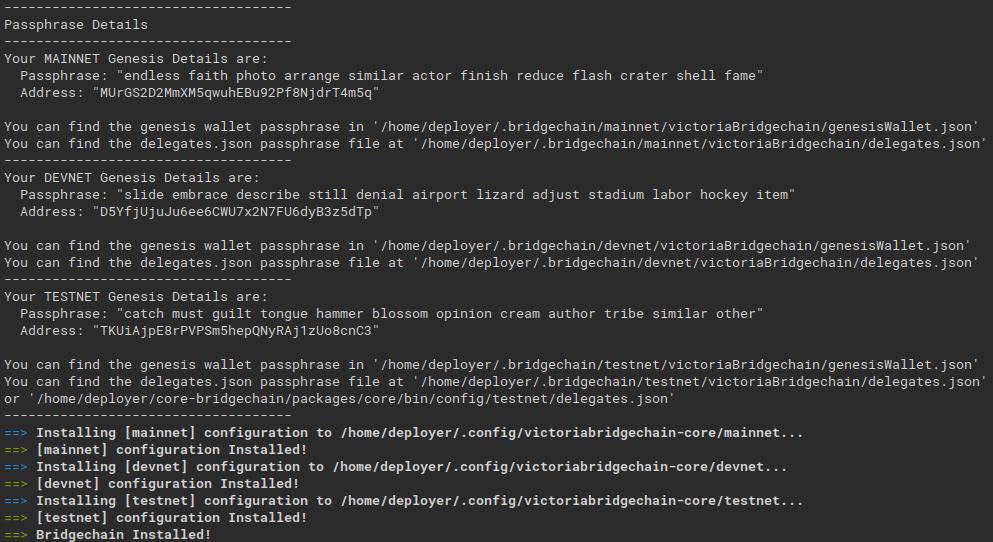
\includegraphics[width=15cm,height=9cm]{figuras/Instalacion_bridgechain.png}
	\caption{Salida tras la instalación del core}
	\label{fig:install-bridge}
\end{figure}

A continuación se instalará el explorer para poder ver las transacciones y bloques generados, código \ref{cod:install-explorer}.

\begin{lstlisting}[language=Bash,caption=Instalación \textit{blockchain}. Parte XII, label=cod:install-explorer, style=Consola]
	$ ./deployer/bridgechain.sh install-explorer --config deployer/config.sample.conf --skip-deps --non-interactive
\end{lstlisting}


El último paso es iniciar la \textit{blockchain} y el \textit{explorer}, código \ref{cod:start-brid}. La salida tras iniciar el \textit{explorer} la muestra la imagen \ref{fig:install-explorer}, que son los estados de la \textit{blockchain} y del \textit{explorer}. Esto mismo se visualizar con el comando \texttt{pm2 status}.\\

\begin{lstlisting}[language=Bash,caption=Instalación \textit{blockchain}. Parte XIII, label=cod:start-brid, style=Consola]
	$ ./deployer/bridgechain.sh start-core --network testnet

	==> Starting...
	Starting victoriabridgechain-relay... done
	Starting victoriabridgechain-forger... done
	==> Start OK!


	$ ./deployer/bridgechain.sh start-explorer --network testnet
\end{lstlisting}


\begin{figure}[H]
	\centering
	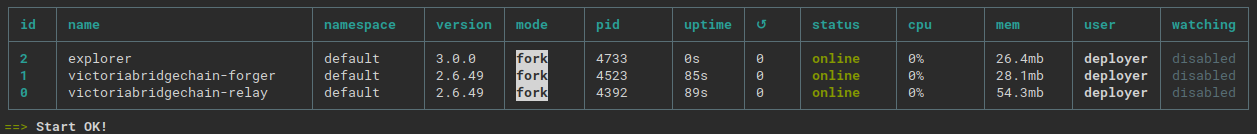
\includegraphics[width=14.5cm,height=2cm]{figuras/Instalacion_explorer.png}
	\caption{Salida tras iniciar del \textit{explorer}}
	\label{fig:install-explorer}
\end{figure}

Para visualizar las transacciones en el \textit{explorer}, debemos de abrir un navegador y acceder a la url \texttt{http://NODE\_GENESIS\_IP:EXPLORER\_PORT}, donde el \texttt{EXPLORER\_PORT} es $4200$. La imagen \ref{fig:nav-explorer} muestra las primeras transacciones realizadas, entre ellas se encuentra la transacción inicial al monedero génesis, además del registro de los delegados.

\begin{figure}[H]
	\centering
	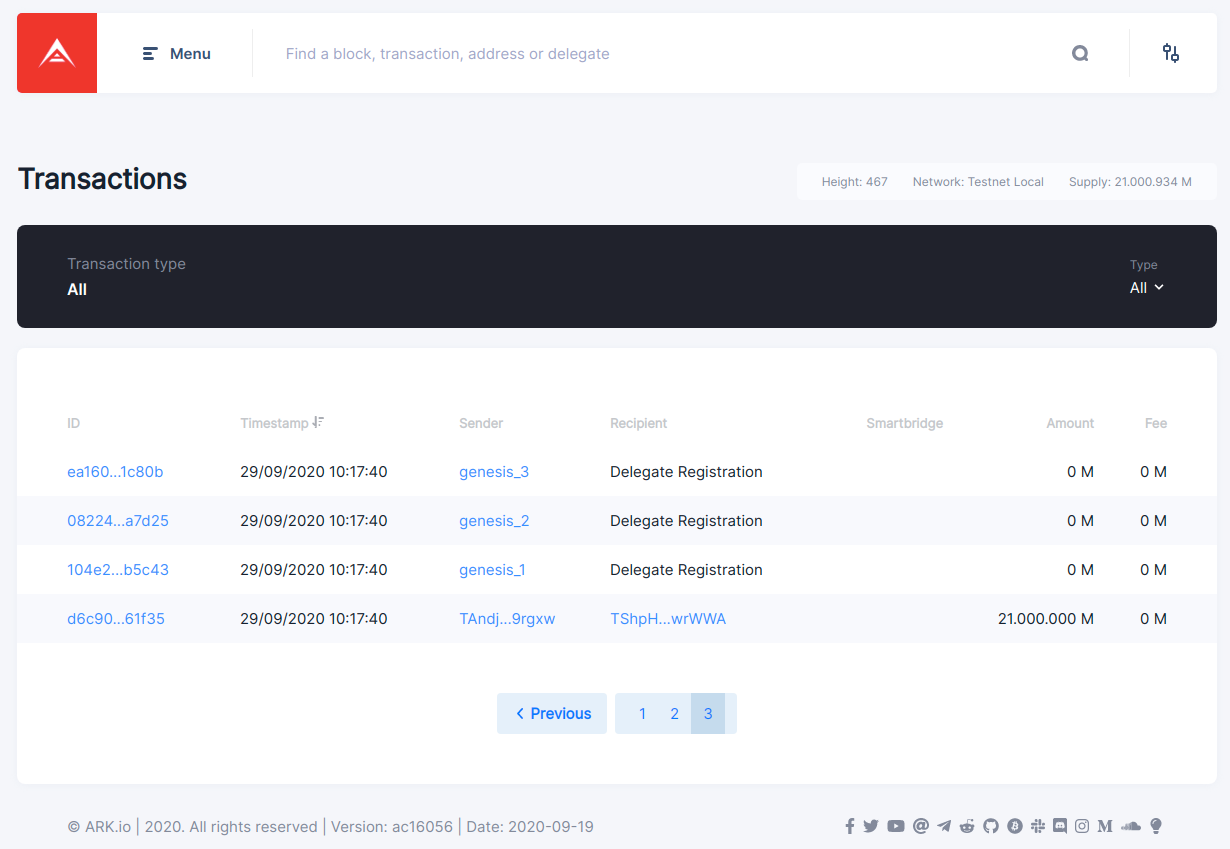
\includegraphics[width=14.5cm,height=10.5cm]{figuras/Navegacion_explorer.png}
	\caption{Primeras transacciones en el \textit{explorer}}
	\label{fig:nav-explorer}
\end{figure}


\newpage
\section{Instalación de la aplicación ARK Desktop Wallet}
\label{sec:manual-wallet}

Antes de descargar la aplicación ARK Desktop Wallet, en el ordenador local, son necesarias algunas instalaciones previas, como algunos archivos de desarrollo de \texttt{libudev}, \texttt{node 12} y \texttt{yarn}, código \ref{cod:install-wallet}.

\begin{lstlisting}[language=Bash,caption=Instalaciones previas a la aplicación ARK Wallet, label=cod:install-wallet, style=Consola]
$ sudo apt-get install libudev-dev libusb-1.0-0-dev

$ npm install -g n
$ sudo n 12

# Para comprobar que se ha instalado node 12
$ n --version

$ npm install -g yarn
\end{lstlisting}

La descarga de la aplicación se realiza desde el repositorio de github de \texttt{@ArkEcosystem/desktop-wallet} \cite{descargas-wallet}, para el proyecto se ha descargado la última versión del archivo \texttt{.deb}.

\begin{lstlisting}[language=Bash,caption=Instalación de la aplicación ARK Wallet, label=cod:install-wallet, style=Consola]
$ sudo dpkg -i ark-desktop-wallet-linux-amd64-<VERSION>.deb

#Para desintalarlo
$ sudo apt-get remove ark-desktop-wallet
\end{lstlisting}


Una vez que se ha instalado la aplicación, la abrimos y nos encontramos con la imagen \ref{fig:wallet-1}. A continuación, vamos siguiendo los pasos que nos salen en la parte de la derecha de la pantalla.

\begin{figure}[H]
	\centering
	
\includegraphics[width=13.5cm,height=7.5cm]{figuras/wallet_1.png}
	\caption{Inicio de Wallet}
	\label{fig:wallet-1}
\end{figure}

\newpage
Así se llega al primer paso, crear un perfil, en el que hay que indicar el nombre y la moneda con la que se quiere trabajar, en este caso se dejan los valores por defecto, además existe la opción de cambiar el avatar del usuario, imagen \ref{fig:wallet-2}.

\begin{figure}[H]
	\centering
	\tcbox[colback=white, colframe=codegray]{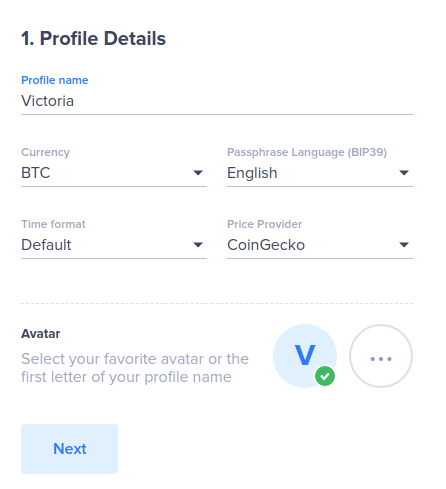
\includegraphics[width=6cm,height=7cm]{figuras/wallet_2.png}}
	\caption{Detalles del perfil}
	\label{fig:wallet-2}
\end{figure}

En el siguiente paso aparece un menú con las posibles redes, \textit{mainnet} y \textit{devnet}. Sin embargo, si se desea usar la red \textit{testnet} es necesario crearla pulsando nueva red. Los campos a rellenar son el nombre, una breve descripción y la dirección del servidor con el puerto de la API, \texttt{http:/GENESIS\_NODE\_IP:API\_PORT}, imagen \ref{fig:wallet-3}.

\begin{figure}[H]
	\centering
	\tcbox[colback=white, colframe=codegray]{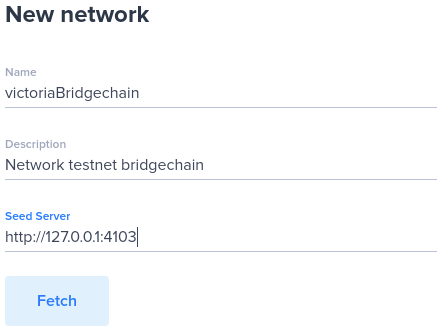
\includegraphics[width=6cm,height=5cm]{figuras/wallet_3.png}}
	\caption{Configuración de la nueva red}
	\label{fig:wallet-3}
\end{figure}

\newpage
Cuando se ha creado la red aparece una pantalla con los detalles de la misma donde debemos de cambiar la dirección por defecto del explorer y poner \texttt{http://GENESIS\_NODE\_IP:EXPLORER\_PORT}. También se pueden cambiar el nombre de los Tokens y el símbolo. Una vez realizados los cambios, guardamos la red, imagen \ref{fig:wallet-4-5}.

\begin{figure}[H]
	\centering
	\begin{minipage}{0.4\textwidth}
		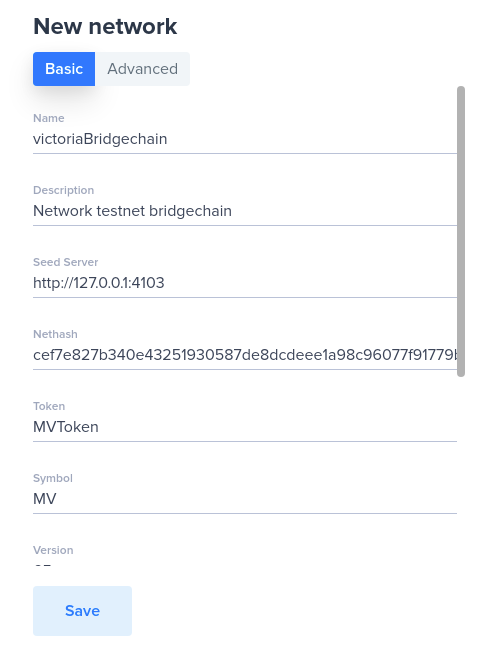
\includegraphics[width=6.5cm,height=8.5cm]{figuras/wallet_4.png}
	\end{minipage}\vfill
	\begin{minipage}{0.38\textwidth}
		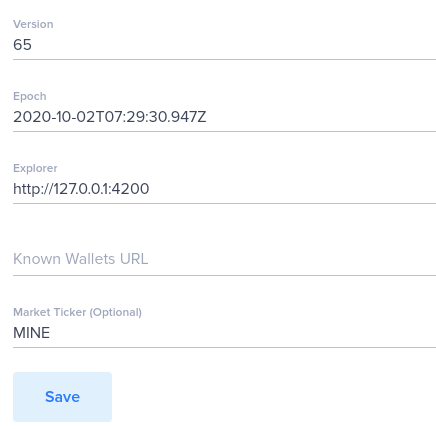
\includegraphics[width=6.3cm,height=8.5cm]{figuras/wallet_5.png}	
	\end{minipage}
	\caption{Detalles de la nueva red}
	\label{fig:wallet-4-5}
\end{figure}

\newpage
Se selecciona la red recien creada, \texttt{victoriaBridgechain} y se avanza al siguiente paso, imagen \ref{fig:wallet-6}.

\begin{figure}[H]
	\centering
	\tcbox[colback=white, colframe=codegray]{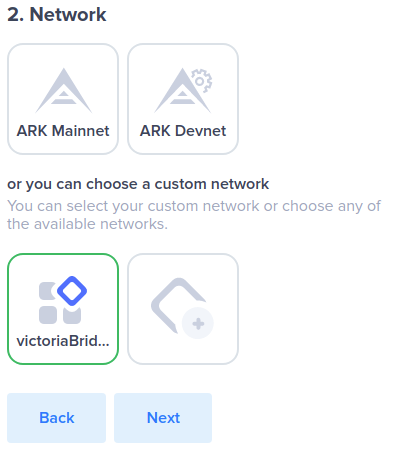
\includegraphics[width=6cm,height=7cm]{figuras/wallet_6.png}}
	\caption{Selección de la red}
	\label{fig:wallet-6}
\end{figure}

Para acabar con la creación del usuario, se tiene la opción de personalizar los colores de la interfaz de usuario o cambiar al tema de noche, imagen \ref{fig:wallet-7}.

\begin{figure}[H]
	\centering
	\tcbox[colback=white, colframe=codegray]{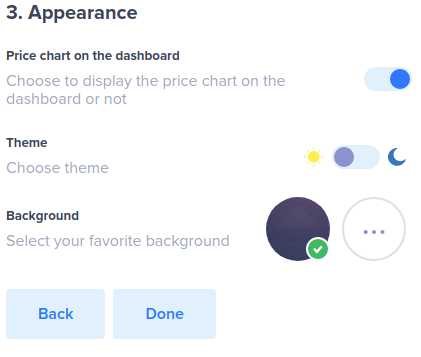
\includegraphics[width=6cm,height=6cm]{figuras/wallet_7.png}}
	\caption{Personalización del diseño de la interfaz}
	\label{fig:wallet-7}
\end{figure}

\newpage
La primera vez que se entra al usuario es necesario importar el monedero que se ha creado durante la instalación de la \textit{blockchain}, pulsando en la esquina superior derecha en \texttt{Import Wallet}. No es necesario rellenar los dos campos, se puede importar el monedero introduciendo solamente la \textit{passphrase}, imagen \ref{fig:wallet-8}.

\begin{figure}[H]
	\centering
	\tcbox[colback=white, colframe=codegray]{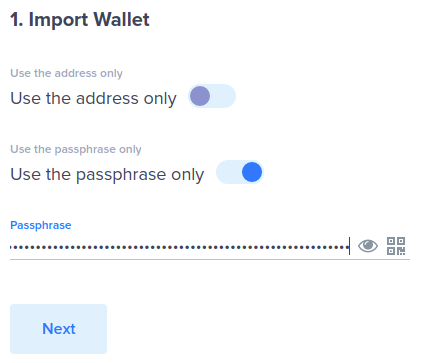
\includegraphics[width=6cm,height=6cm]{figuras/wallet_8.png}}
	\caption{Importar monedero}
	\label{fig:wallet-8}
\end{figure}

Si se desea se puede poner contraseña al monedero, haciéndolo más seguro, en el ejemplo no se van a poner contraseña a ninguno de los monederos, imagen \ref{fig:wallet-9}.

\begin{figure}[H]
	\centering
	\tcbox[colback=white, colframe=codegray]{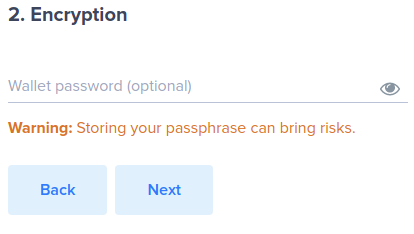
\includegraphics[width=6cm,height=4cm]{figuras/wallet_9.png}}
	\caption{Encriptación el monedero}
	\label{fig:wallet-9}
\end{figure}

\newpage
Finalmente, hay que ponerle nombre al monedero, para diferenciarlo de otros monederos y saber cual es el que contiene la cantidad inicial, el nombre que se le va a poner es \texttt{MainWallet}, imagen \ref{fig:wallet-10}.

\begin{figure}[H]
	\centering
	\tcbox[colback=white, colframe=codegray]{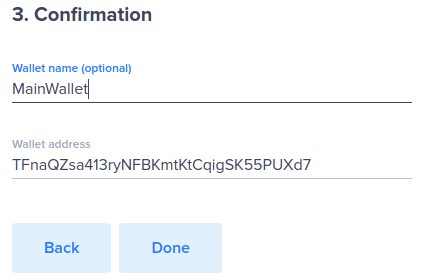
\includegraphics[width=6cm,height=5cm]{figuras/wallet_10.png}}
	\caption{Confirmación para crear el monedero}
	\label{fig:wallet-10}
\end{figure}

Para que salga la cantidad de dinero inicial es necesario conectar la aplicación con la \textit{blockchain}. Pulsando en el panel lateral izquierdo en \texttt{Network}, se accede a la configuración de la red y pulsando en \texttt{Connect custom peer} obtenemos la imagen \ref{fig:wallet-11-12}. Rellenamos los campos con \texttt{http://GENESIS\_NODE\_IP} y con el \texttt{API\_PORT}. Cuando se conecte hay que refrescar la página para que se actualice el monedero con el dinero.

\begin{figure}[H]
	\centering
	\begin{minipage}{0.4\textwidth}
		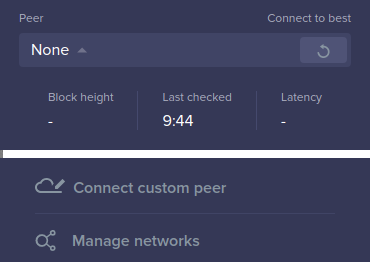
\includegraphics[width=7cm,height=6.5cm]{figuras/wallet_11.png}
	\end{minipage}\hfill
	\begin{minipage}{0.4\textwidth}
		\tcbox[colback=white, colframe=codegray]{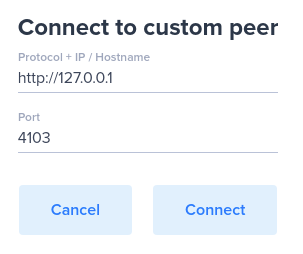
\includegraphics[width=6cm,height=6cm]{figuras/wallet_12.png}}
	\end{minipage}
	\caption{Configuración de la conexión peer}
	\label{fig:wallet-11-12}
\end{figure}

\newpage
Para realizar transacciones y poder probar el algoritmo, es necesario crear otro monedero y realizar transacciones entre ambos. De esta forma, hay que acceder a la sección \texttt{My wallets} y pulsar \texttt{Create Wallet}. El primer paso es introducir el nombre del monedero, imagen \ref{fig:wallet-13}.
 
\begin{figure}[H]
	\centering
	\tcbox[colback=white, colframe=codegray]{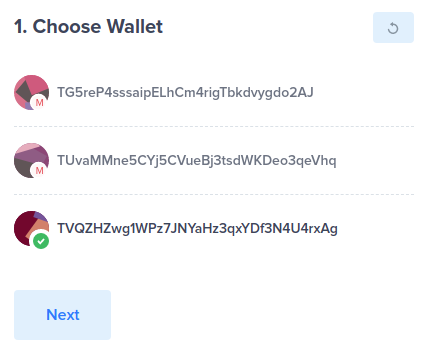
\includegraphics[width=7cm,height=6.5cm]{figuras/wallet_13.png}}
	\caption{Selección de la dirección del nuevo monedero}
	\label{fig:wallet-13}
\end{figure}

La imagen \ref{fig:wallet-14} muestra la \textit{passphrase} del monedero. Esta \textit{passphrase} hay que guardarla, tal y como se hizó con la \textit{passphrase} de monedero importado, pues será necesaria para realizar transacciones posteriormente.

\begin{figure}[H]
	\centering
	\tcbox[colback=white, colframe=codegray]{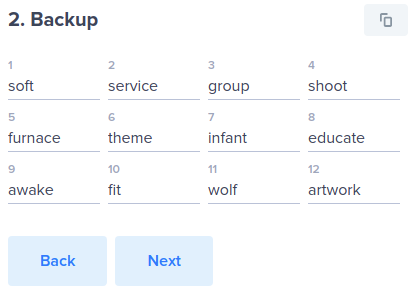
\includegraphics[width=6.5cm,height=5cm]{figuras/wallet_14.png}}
	\caption{\textit{Passphrase} o clave privada del monedero}
	\label{fig:wallet-14}
\end{figure}

\newpage
La verificación de la \textit{passphrase} se hace introduciendo tres palabras, la número tres, seis y nueve, si se desea se puede realizar la verifiación introduciendo todas las palabras, imagen \ref{fig:wallet-15}.

\begin{figure}[H]
	\centering
	\tcbox[colback=white, colframe=codegray]{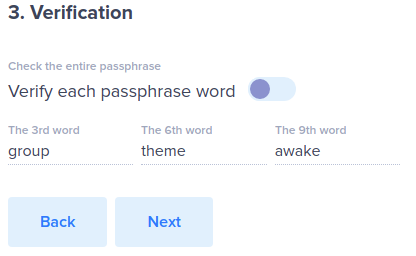
\includegraphics[width=7cm,height=5cm]{figuras/wallet_15.png}}
	\caption{Verificación de la \textit{passphrase}}
	\label{fig:wallet-15}
\end{figure}

Si se desea se puede poner contraseña al monedero, en el ejemplo no es necesario, imagen \ref{fig:wallet-16}.

\begin{figure}[H]
	\centering
	\tcbox[colback=white, colframe=codegray]{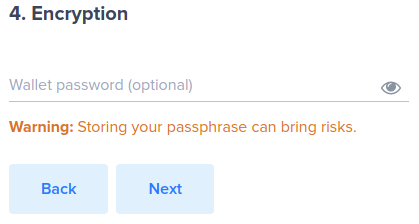
\includegraphics[width=7cm,height=5cm]{figuras/wallet_16.png}}
	\caption{Encriptación del monedero}
	\label{fig:wallet-16}
\end{figure}

\newpage

Antes de confirmar la creación del monedero, hay que introducir el nombre del mismo, \texttt{Second Wallet}, para hacer referencia a que no tendrá ningún token hasta que no reciba una transferencia, imagen \ref{fig:wallet-17}.

\begin{figure}[H]
	\centering
	\tcbox[colback=white, colframe=codegray]{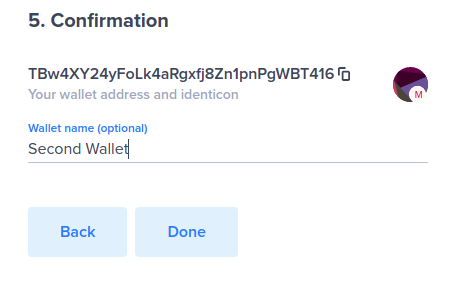
\includegraphics[width=7cm,height=5cm]{figuras/wallet_17.png}}
	\caption{Confirmación para crear el segundo monedero}
	\label{fig:wallet-17}
\end{figure}




%\begin{lstlisting}[language=Bash,caption=Instalación \textit{blockchain}. Parte III, label=cod:suma-cuerpo, style=Consola]

%\end{lstlisting}

\newpage

\section{Visualización de los datos con el Explorer}

\newpage








	\thispagestyle{empty}

\end{document}
